\documentclass{article}
\usepackage[utf8]{inputenc}

%%Let's you change margins
\usepackage[left=1in,right=1in,top=1in,bottom=1in]{geometry}

%%Math symbols, proof environments
\usepackage{amsmath,amsthm,amssymb, graphicx}
\usepackage{subcaption}
\newcommand{\atan}{\tan^{-1}}

%%Use this package for matrices
\usepackage{array}

%%Commands for common sets
\newcommand{\R}{\mathbb{R}} %Real numbers
\newcommand{\Z}{\mathbb{Z}} %Integers

\title{ECE 141 Project} %Remove Template in your title

\author{Inesh Chakrabarti} %Put your name here

\date{\today}

\begin{document}

\maketitle

\subsection*{Problem 1}
Show that for any desired $\beta$ in $[0, 2\pi)$ there exists a $u$ in $[0, 2\pi)$ so that (5) holds. We can thus treat $\beta$ as the input since for any $\beta$ computed by a controller we can compute the steering angle $u$ via the relation (5) and apply this command to the motor steering for the wheels. This will greatly simplify the equations you have to work with.
\begin{proof}[Solution]
First, let us look at relation (5):
\[\beta = \atan\left(\dfrac{\ell_r}{\ell_r+\ell_f}\tan(u)\right)
\]
Note that we know $\ell_f = 1.1m$ and $\ell_r = 1.7m$, so subsitututing, we are left with 
\[\beta = \atan\left(\dfrac{1.7}{1.7+1.1}\tan(u)\right)= \atan(k\tan(u))
\]
where $k=\dfrac{1.7}{2.8} \approx 0.607142857$ \newline
Note that the range of $\tan(u)$ for $u \in [0, 2\pi)$ is all real numbers, so the range of $k\tan(u)$ must also be all real numbers. Therefore, we can deal with $\atan$ function's regular range, as we have included all numbers in its domain. Assuming that the given $\atan$ refers to a four quadrant tangent inverse function, we thus arrive at the conclusion that for any desired $\beta \in [0, 2\pi)$ there exists some $u \in [0, 2\pi)$
\end{proof}

\subsection*{Problem 2}
We first consider the lane keeping problem, i.e., the design of a controller that keeps the car in the center of its lane. For this purpose we assume the car’s velocity to be constant at 35 mph, that the lane center corresponds to $y = 0$, and that we have a sensor measuring $y$ (in reality, the position of the car on the lane would be computed by using vision to detect the location of the lane markers). Linearize the equations of motion and design a controller that stabilizes the car at $y = 0$ using the linearized model (use the transfer function from $\beta$ to $y$). You don’t need to work with equation (1) since $x$ will not be at equilibrium. Provide some plots showing the controller works as intended.
\begin{proof}[Solution]

First we note that the equations we must linearize are:
\[\dot{y} = v\sin(\psi+\beta)
\]
\[\dot{\psi} = \frac{v}{\ell_r}\sin(\beta)
\]
Let us now try to find a value to linearize these equations around. It makes sense to linearize these equatoins around $\psi = 0$ and $\beta = 0$, as most of our values for these two angles will fall near these values, especially since we are trying to straighten teh car in the lane.
\newline
Then, we can use the small-angle approximation, which holds true around $0$, use the approximations:
\[\sin(\psi+\beta) \approx \psi+\beta 
\]
\[\sin(\beta) \approx \beta
\]
Thus, our linearized equations are:
\[\dot{y} = v(\psi + \beta)
    \]
\[\dot{\psi} = \frac{v\beta}{\ell_r}\]

Note that the velocity of the car for this question is $35$ mph, which is the same as $15.6464$ m/s. We can also calculate $\frac{v}{\ell_r}=\frac{15.6464}{1.7}=9.2038$. \newline
Now, let us determine what it means for the controller to work as intended. For the controller to work as intended, we must haev that the car does not respond too fast; this means that it should not jerk immediately to correct itself. Thus, we can set a constraint for $t_r > 0.1$s, except for specific cases where it is normal for correction to occur very fast (such as when y = 0 and only the angle is different). However, we also want to minimize overshoot to some value, as the car may swerve with excessive overshoot, which is undesirable. Thus, let us arbitarily set a maximum overshoot of $0.5$m, which is about half a meter, an amount most people would be comfortable having the car adjust by. However, I will limit the car to one noticable oscillation, where noticable is any oscillation above 0.1. \newline
Let us now determine what valid inital conditions for $y$ and $\psi$ would be. It makes sense to limit $y$ to small values. Considering the next question uses lanes $3$ m wide, let us use $y \in [-1.5,1.5]$. Similarily, let us consider the range for $\psi$. Similarily, we can arbitarily decide $\psi \in \left[-\frac{pi}{3},\frac{pi}{3}\right]$, which is approximately $\psi \in [-1,1]$. Now we can use simulink to simulate our model. \newline

\begin{figure}[h!]
    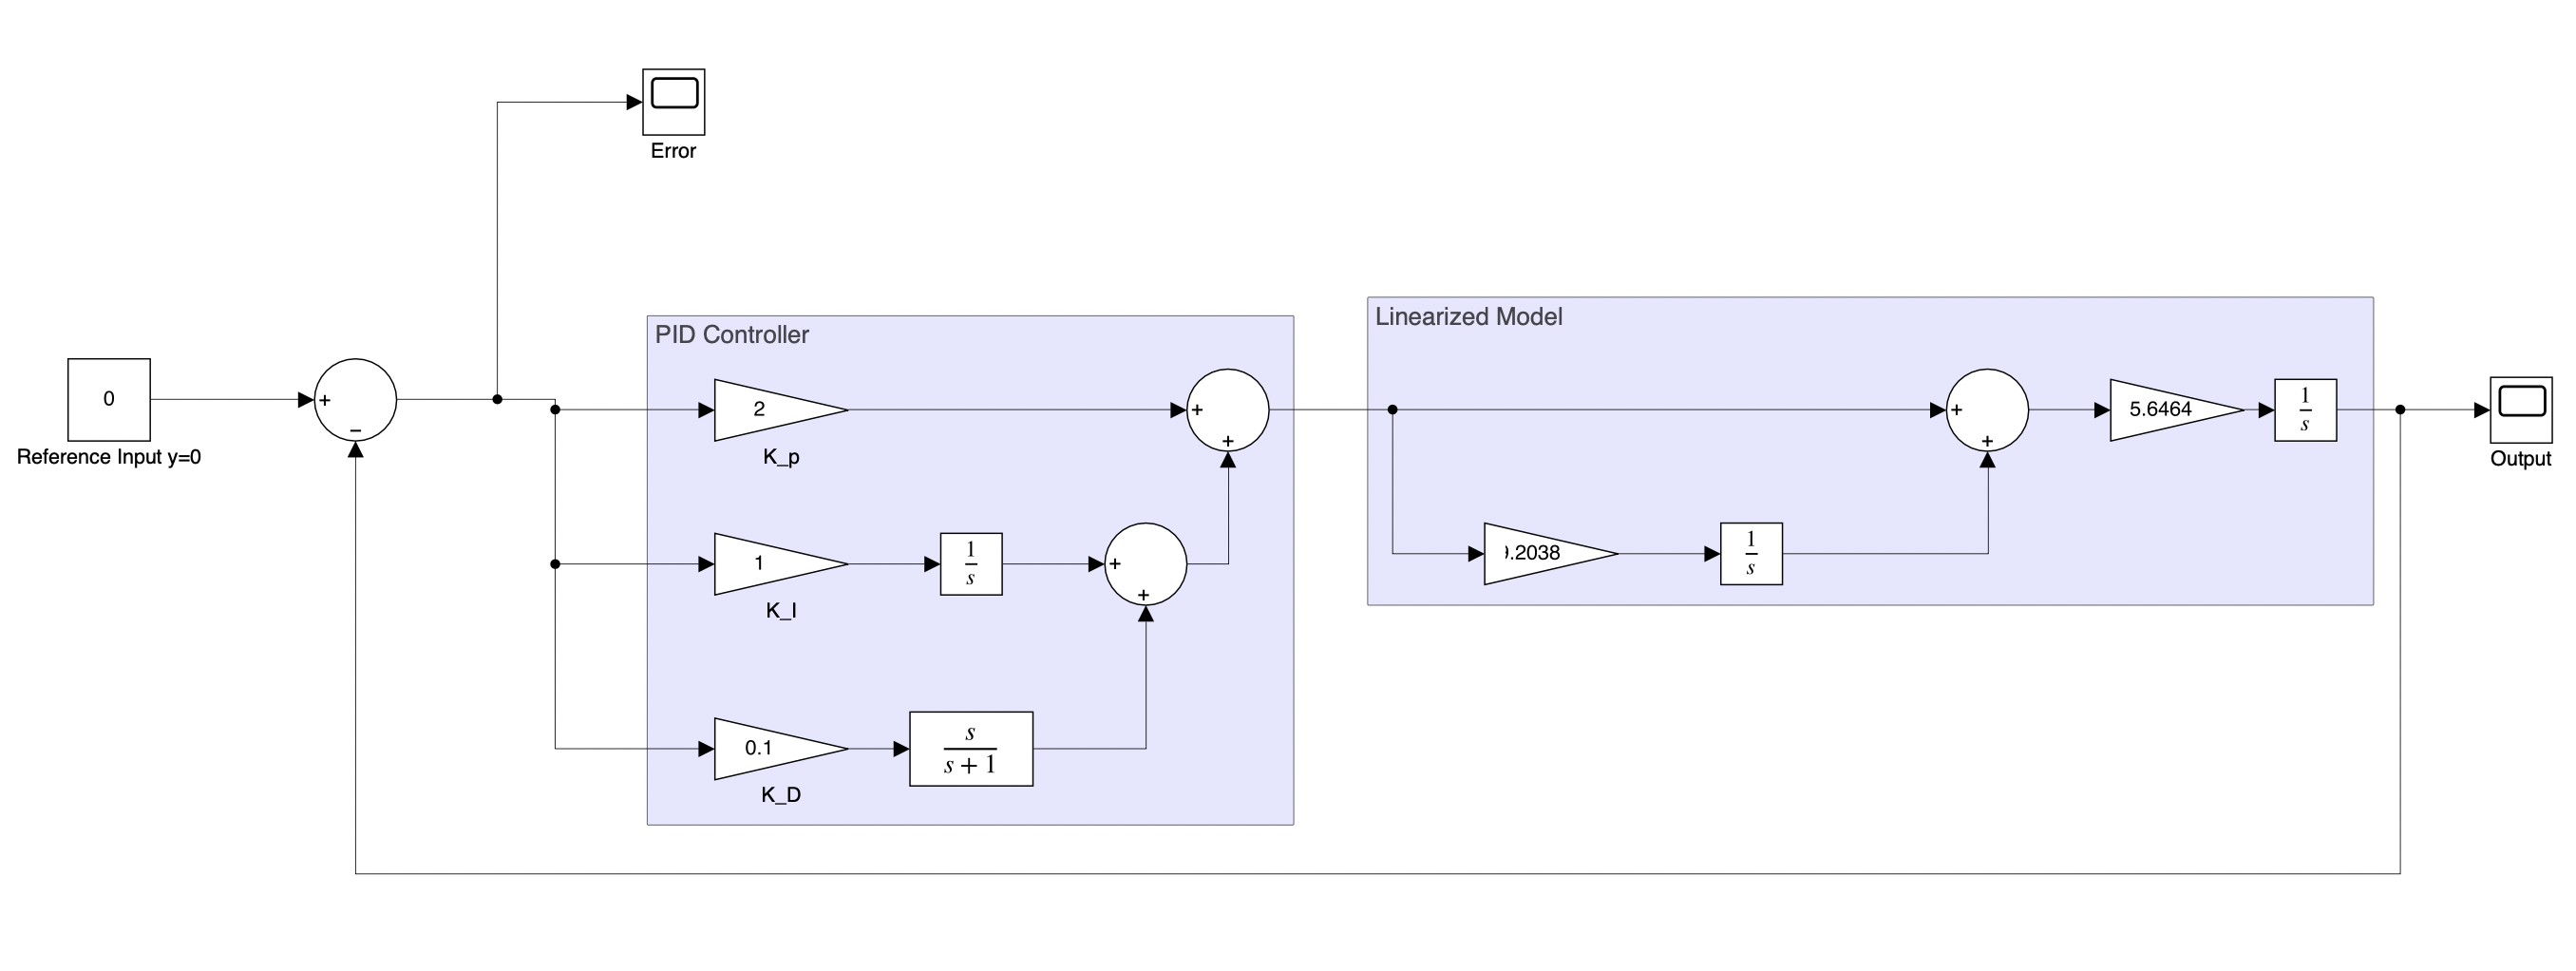
\includegraphics[width=\linewidth]{ECE141Q2Model.png}
    \caption{Linearized Simulink Diagram}
\end{figure}

Figure 1 dispalys the simulink block diagram we used for our linearized model. Note that we have used a PID controller. 
Now let us apply inputs to this controller to different initial conditions to observe the controller behavior:
\begin{figure}[h!]
    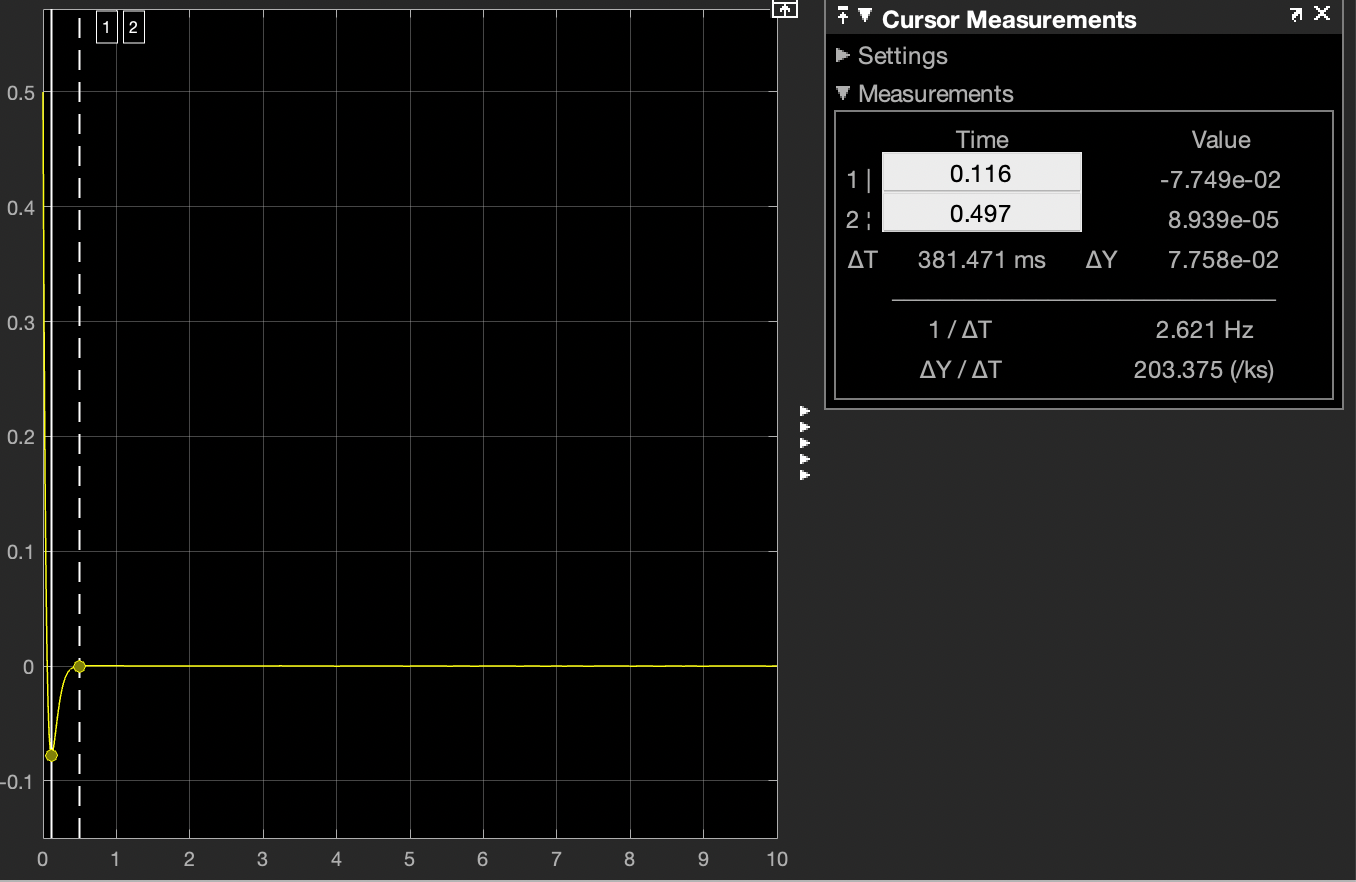
\includegraphics[width=\linewidth]{img1.png}
    \caption{Step Response for Controller}
\end{figure}
First, note that there is zero steady state error with a step input in unity feedback. We also see that it meets all of our required conditions. Next, let us observe the controller's response to differnet initial conditions. 
\newpage
\begin{figure}
    \centering
    \begin{subfigure}{0.4\linewidth}
      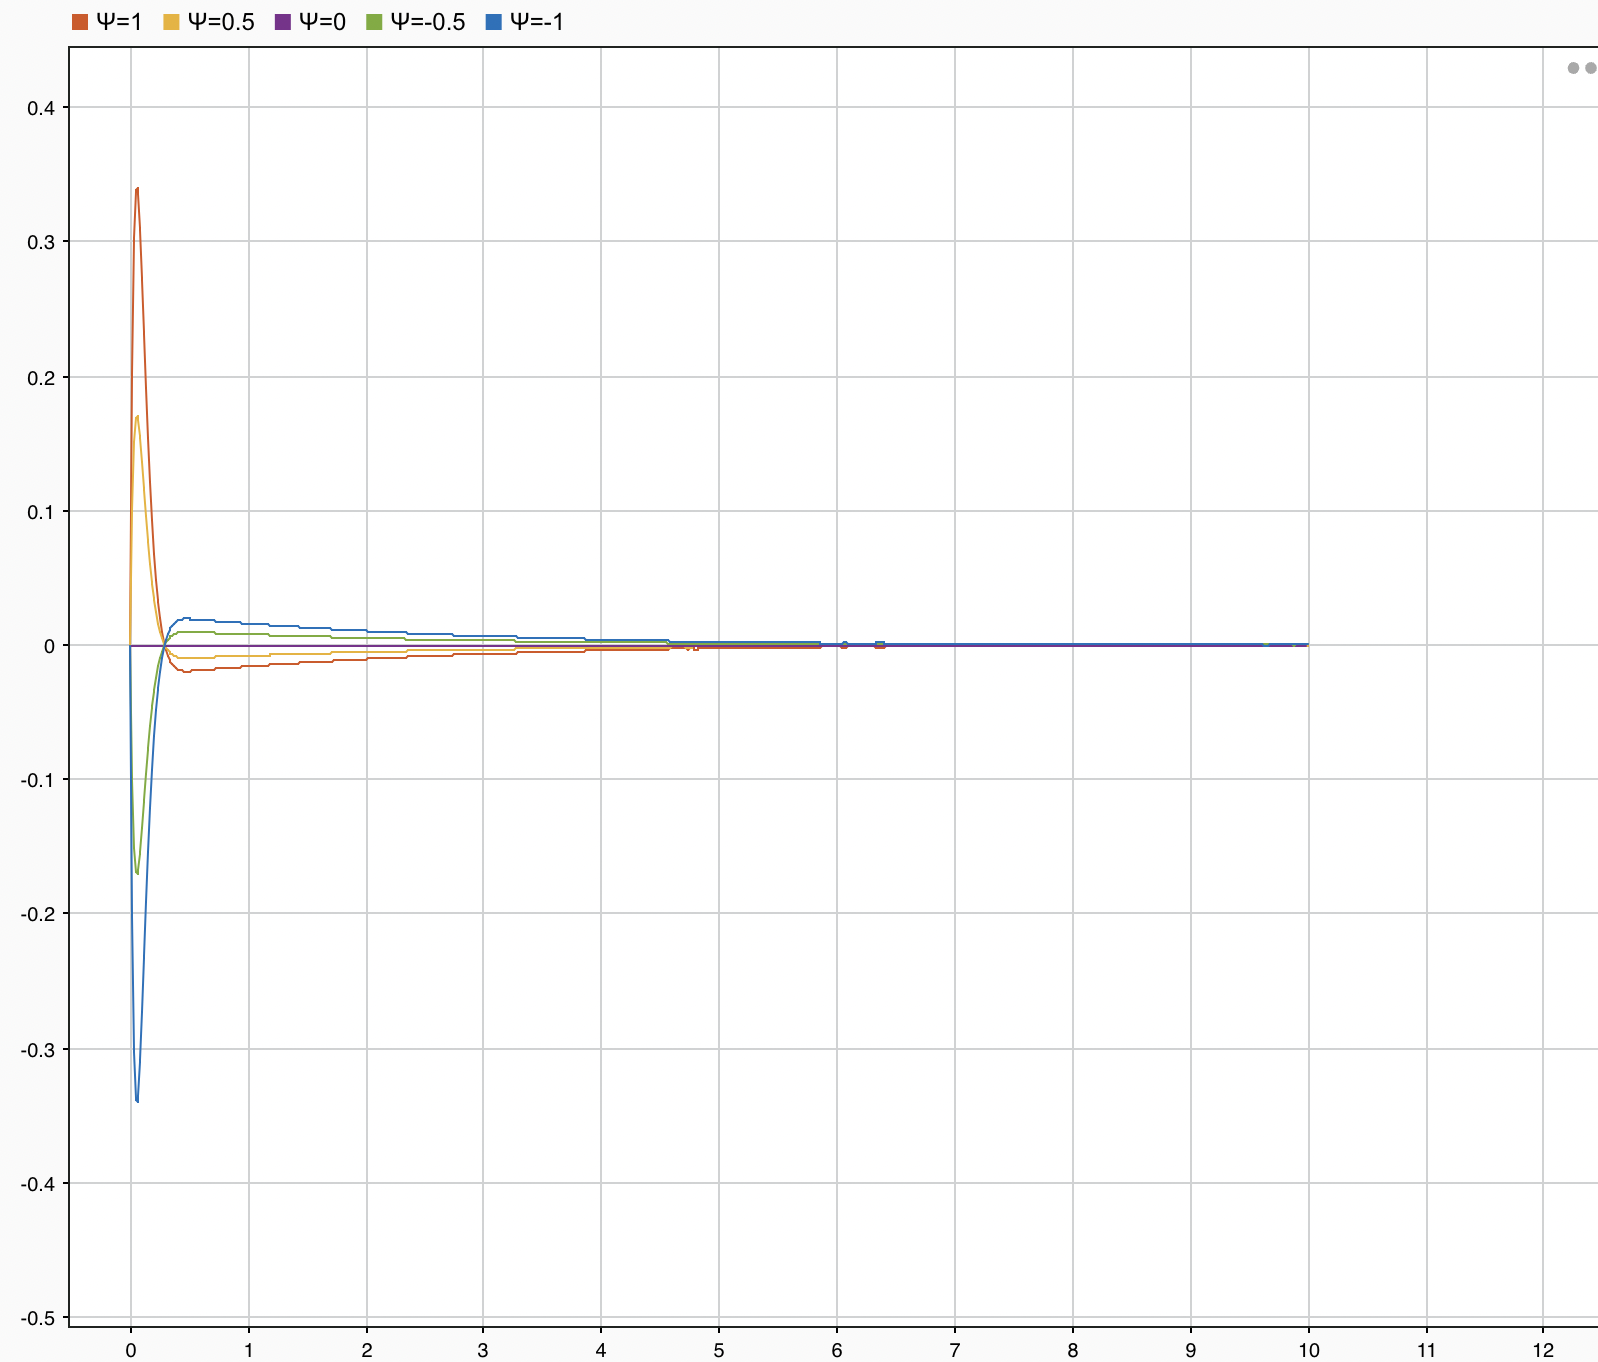
\includegraphics[width=\linewidth]{img2.png}
      \caption{Plots for y=0}
    \end{subfigure}
    \begin{subfigure}{0.4\linewidth}
      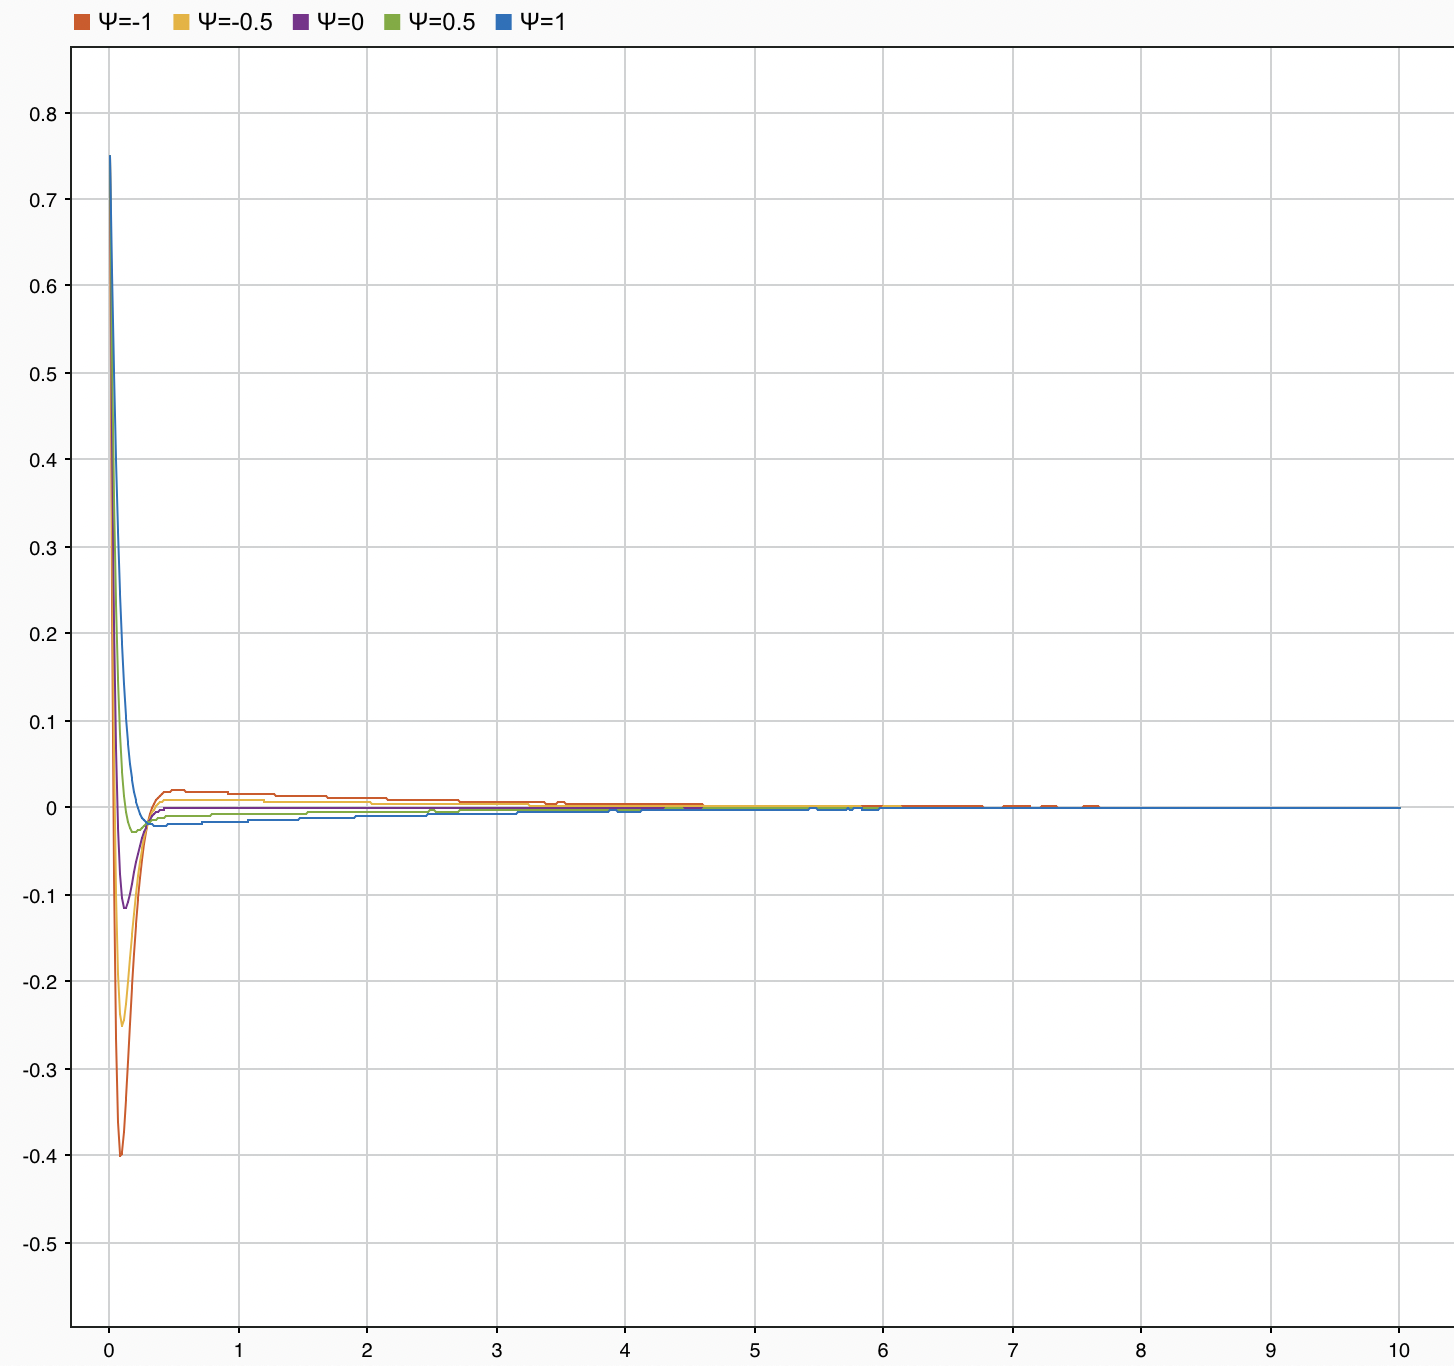
\includegraphics[width=\linewidth]{img3.png}
      \caption{Plots for y=0.75}
    \end{subfigure}
    \begin{subfigure}{0.4\linewidth}
        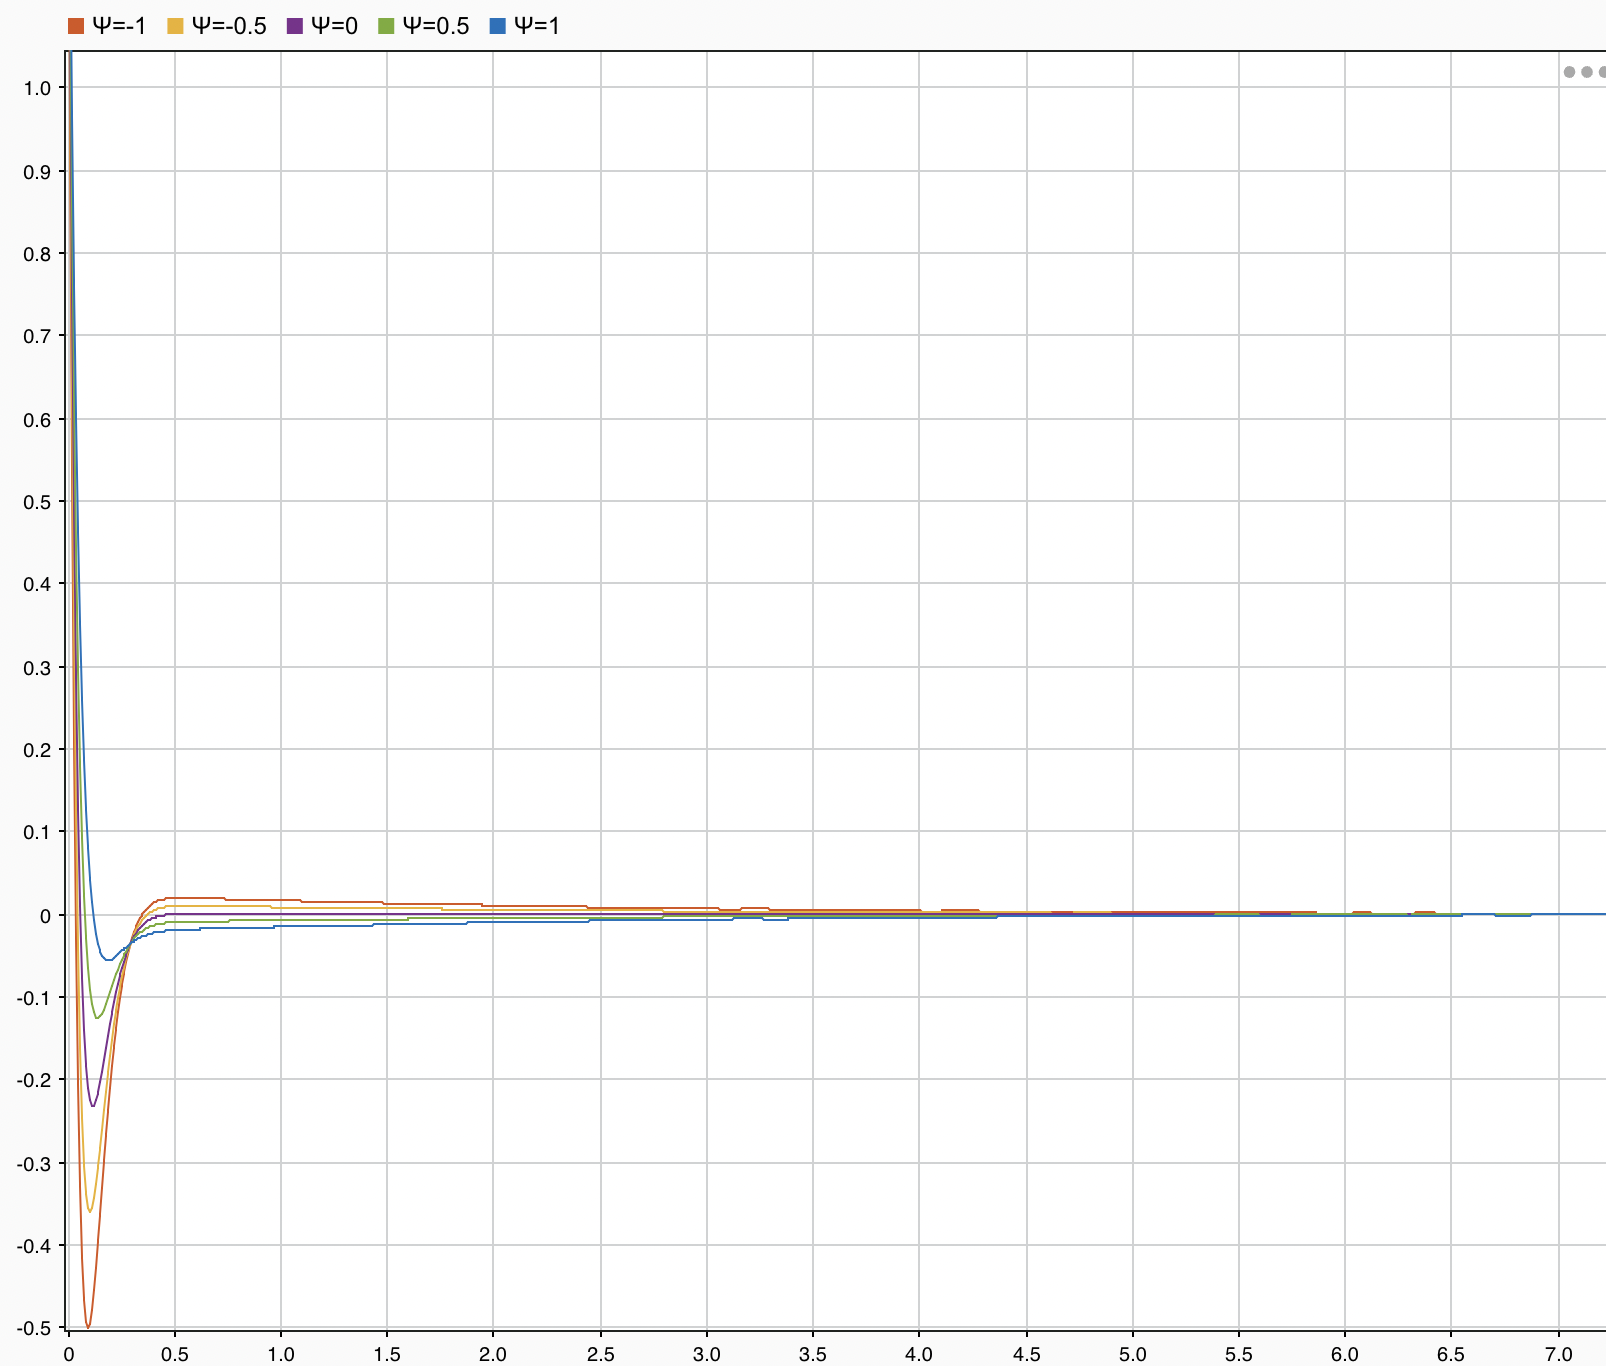
\includegraphics[width=\linewidth]{img4.png}
        \caption{Plots for y=1.5}
      \end{subfigure}
      \begin{subfigure}{0.4\linewidth}
        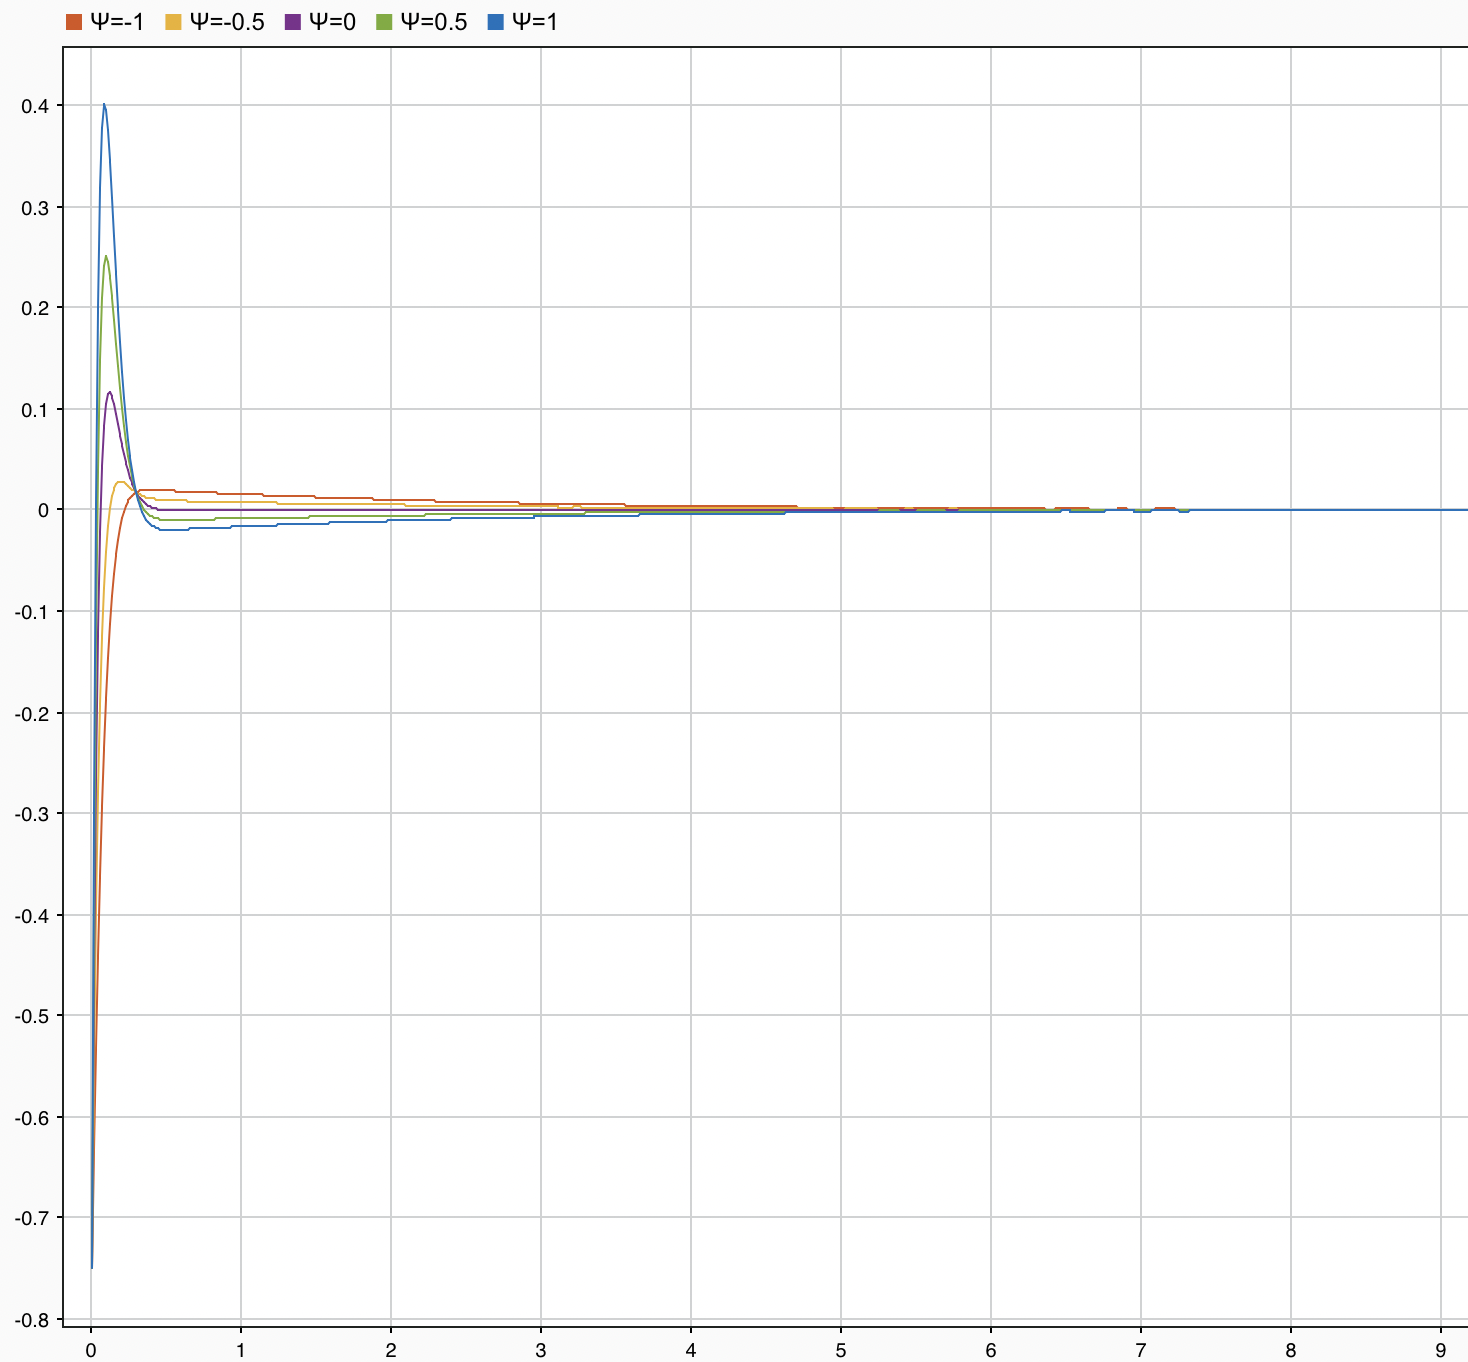
\includegraphics[width=\linewidth]{img5.png}
        \caption{Plots for y=-0.75}
      \end{subfigure}
      \begin{subfigure}{0.4\linewidth}
          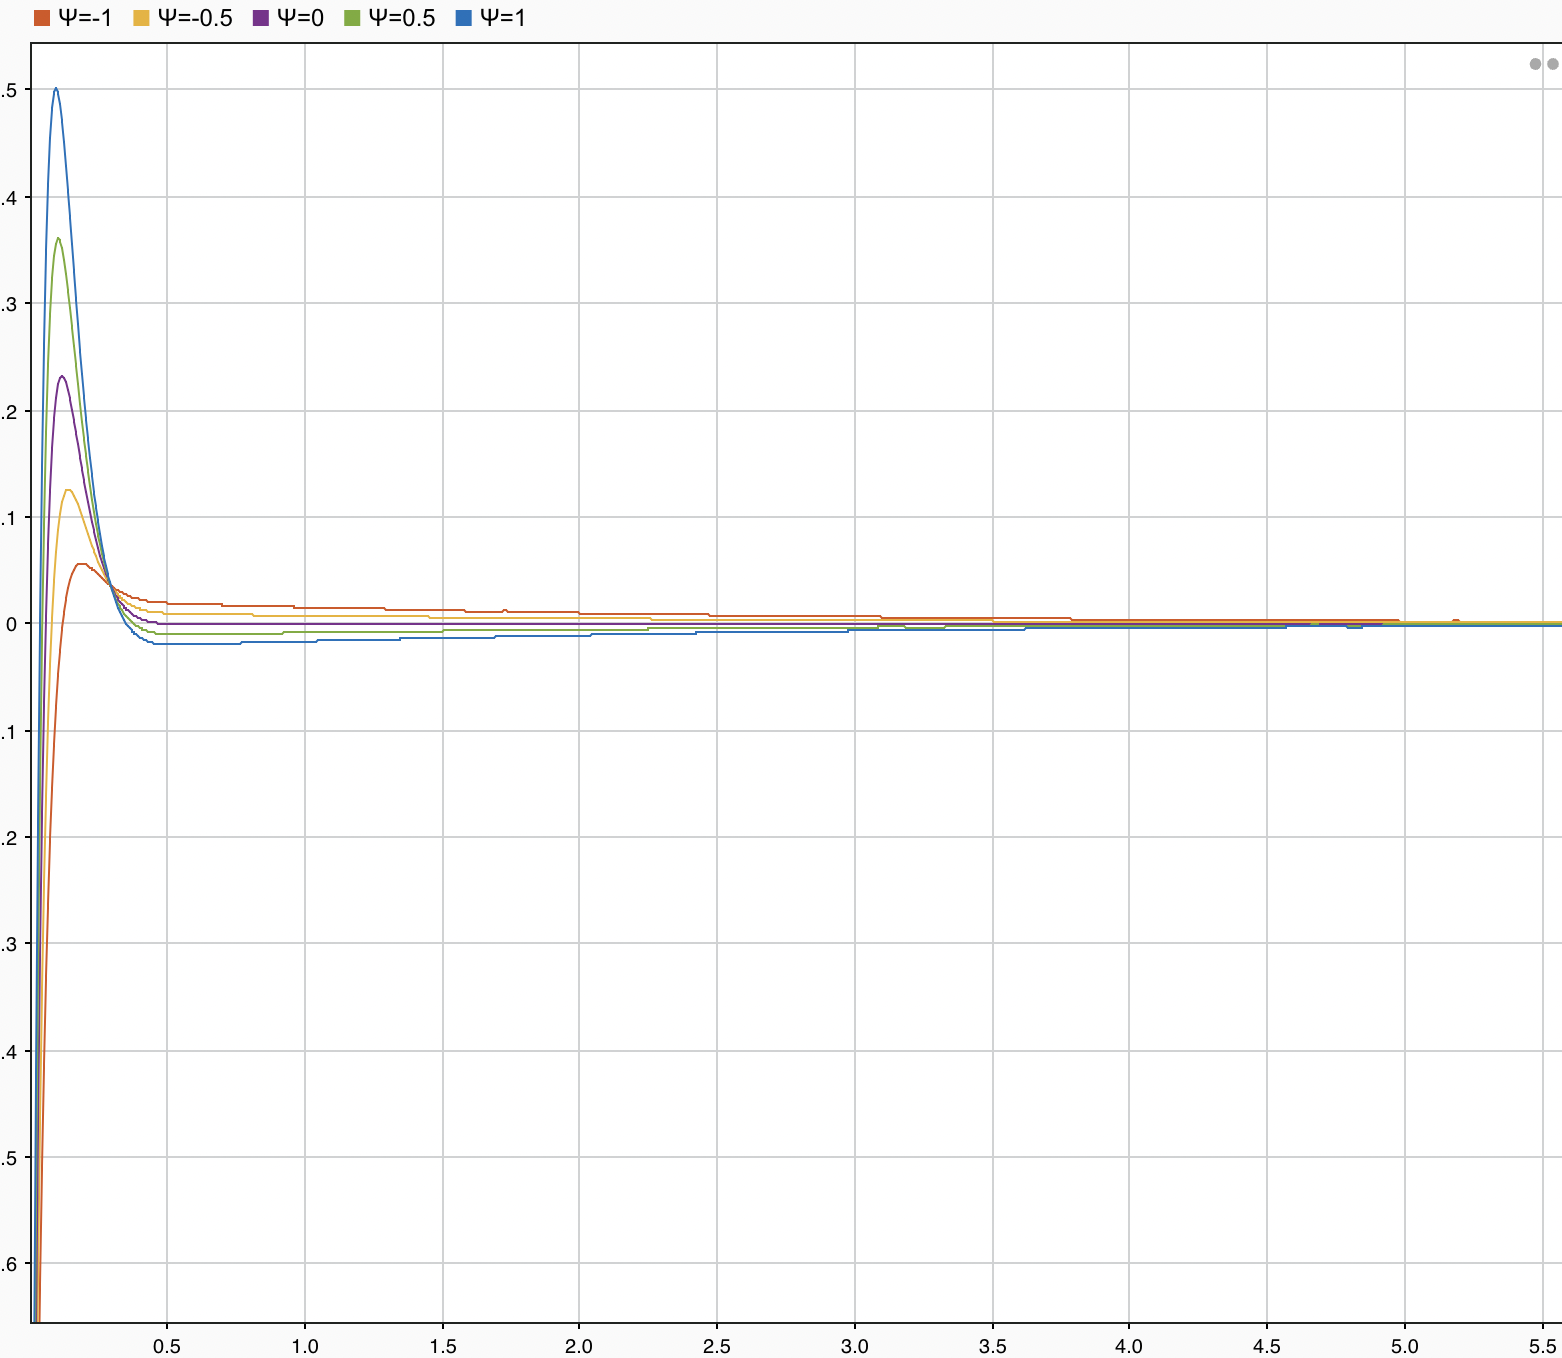
\includegraphics[width=\linewidth]{img6.png}
          \caption{Plots for y=-1.5}
        \end{subfigure}
    \caption{Plots for different initial conditions}

  \end{figure}
We note that our controller does work as intended and meet all of our conditions. (Refer to Figure 3.)
\end{proof}
\newpage
\subsection*{Problem 3}
Simulate the controller from the previous question with the nonlinear car model. Deter-
mine the range of initial conditions for which the controller has adequate performance.
Define what you consider adequate performance for a lane that is 3 meters wide and an
autonomous car that is 1.8 meters wide. Provide some plots to justify your answer.
\begin{proof}[Solution]
To begin this problem, first we have the Simulink block diagram for our nonlinear model in Figure 4.
\begin{figure}[h!]
    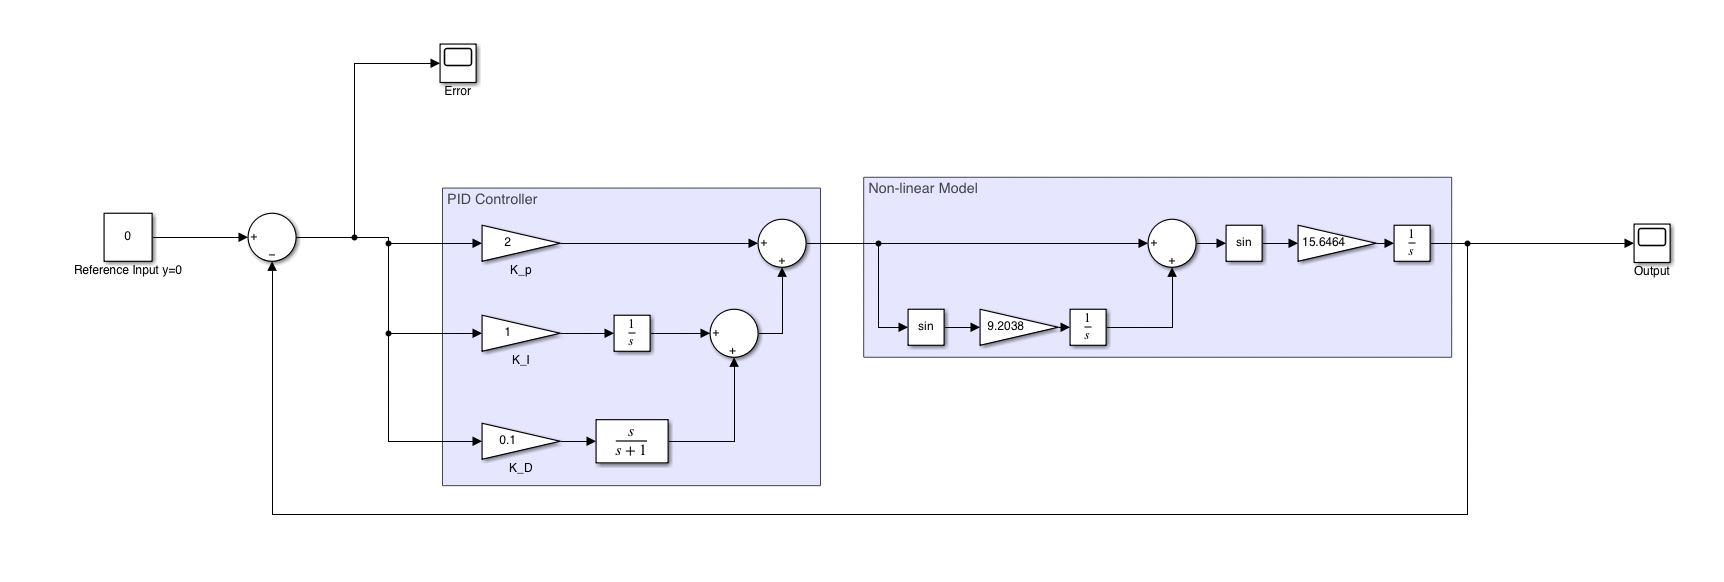
\includegraphics[width=\linewidth]{Q3Model.png}
    \caption{Non-linear Simulink Diagram}
\end{figure}
Our limiting condition for this problem will be to make sure there is no drastic swerving of the car, and to make sure that the car remains in the lane. For this to happen, overshoot must be less than 0.6
Also, we will abide by the same rules for settling time as before to avoid drastic turns. 
\newline
Now, let us attempt to find the range of values for which our controller is acceptable. 
First, let us solve for a maximum $|y|$. Note we know $y \in (-0.6,0.6)$ as we get $\frac{3-1.8}{2}=0.6$.
Let us use the pythagorean theorem for the back of the car, so we get $\sqrt{1.7^2+1.8^2}=2.476$. Let us use the position where this distance is maximized to also 
gauge the maximum $\psi$, as it is unreasonable for the back of the car to turn any more. Thus, we have 
$\atan\left(\frac{1.8}{1.7}\right)=0.814\approx 0.8$. Thus, we have:
 \[y \in (-0.6, 0.6)\]  
 \[\psi \in (-0.8, 0.8)
 \]
 Now, let us plot and see for which values in these inital value ranges our controller is acceptable. We see in Figure 5 that 
 for our given range, our controller is acceptable. There is no overshoot over 0.4, and there is at most one significant oscillation. This means the car is not swerving.
 Also, rise time is greater than 0.1 seconds in all all of the plots, so the movement is not jerky.
 \begin{figure}
    \centering
    \begin{subfigure}{0.4\linewidth}
      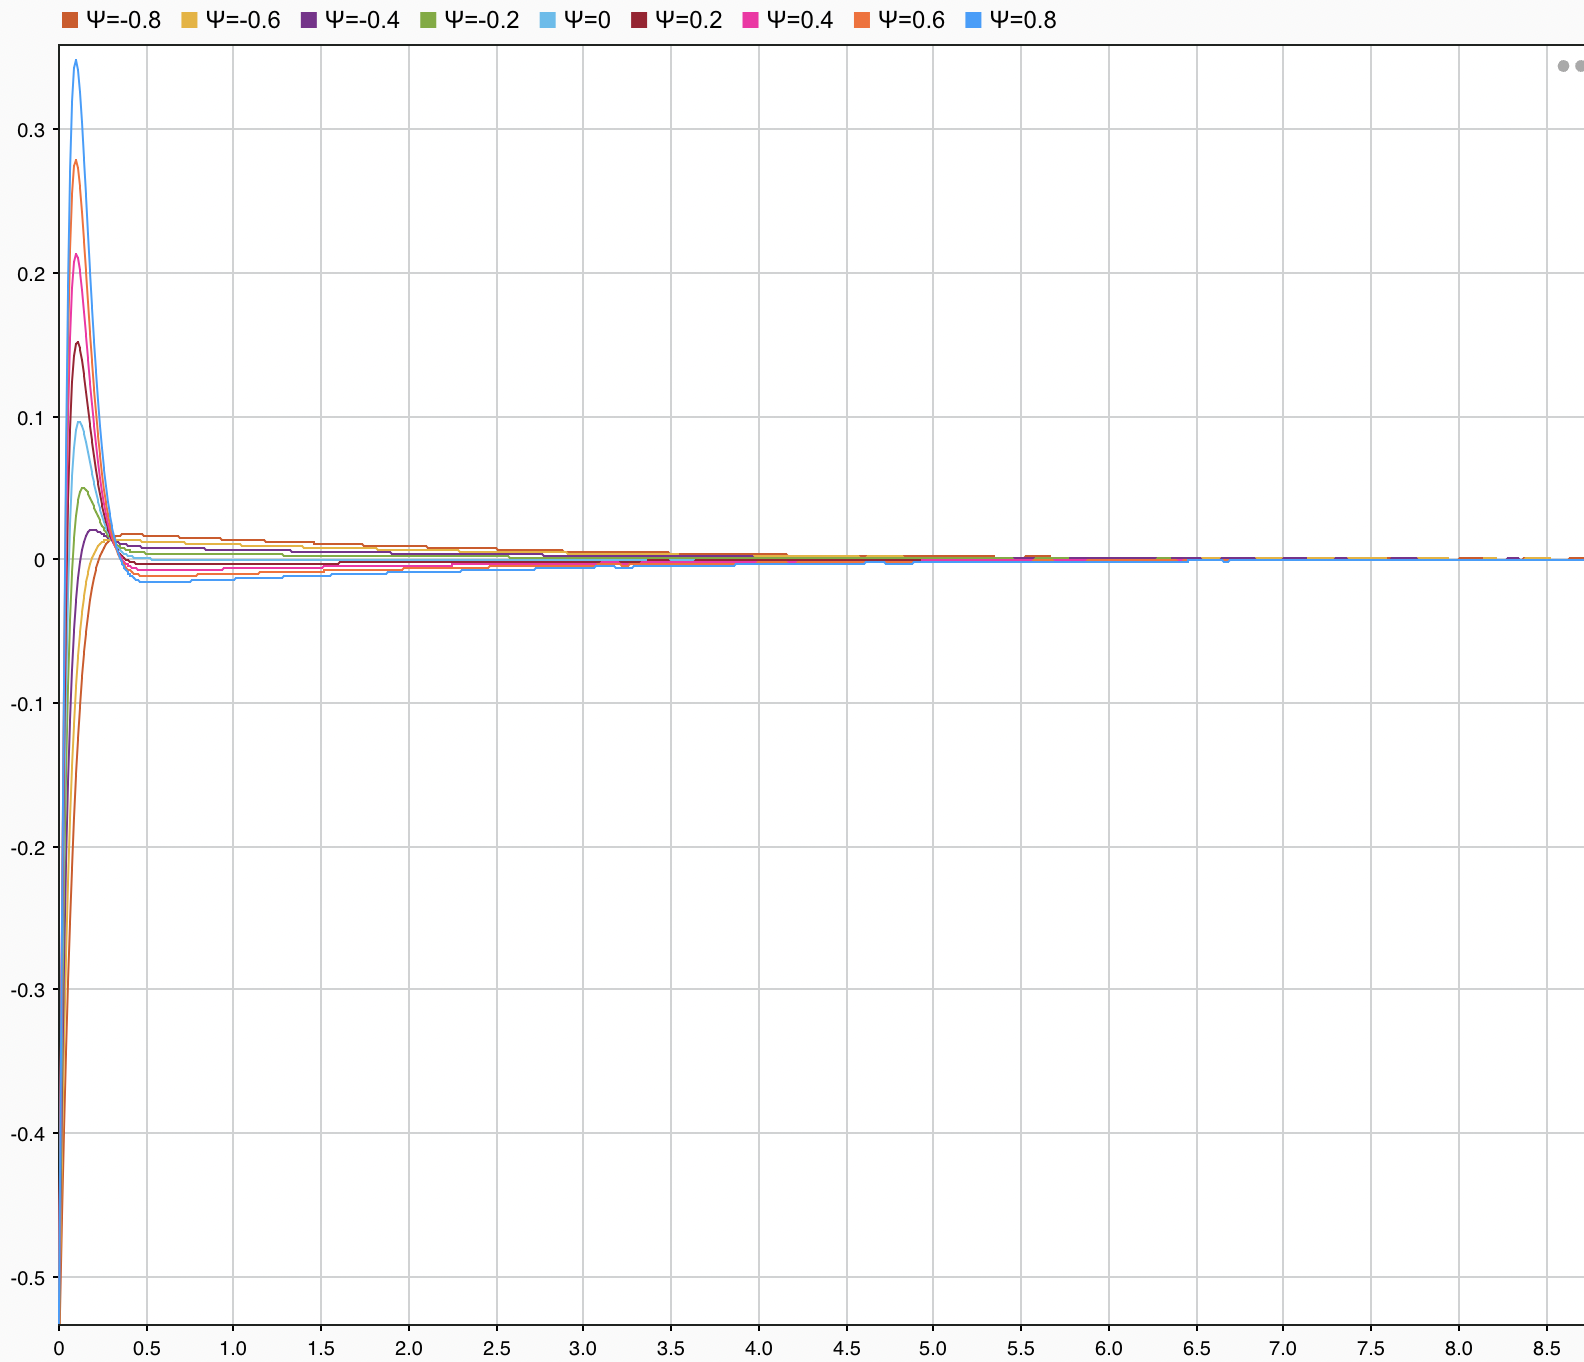
\includegraphics[width=\linewidth]{img7.png}
      \caption{Plots for y=-0.6}
    \end{subfigure}
    \begin{subfigure}{0.4\linewidth}
      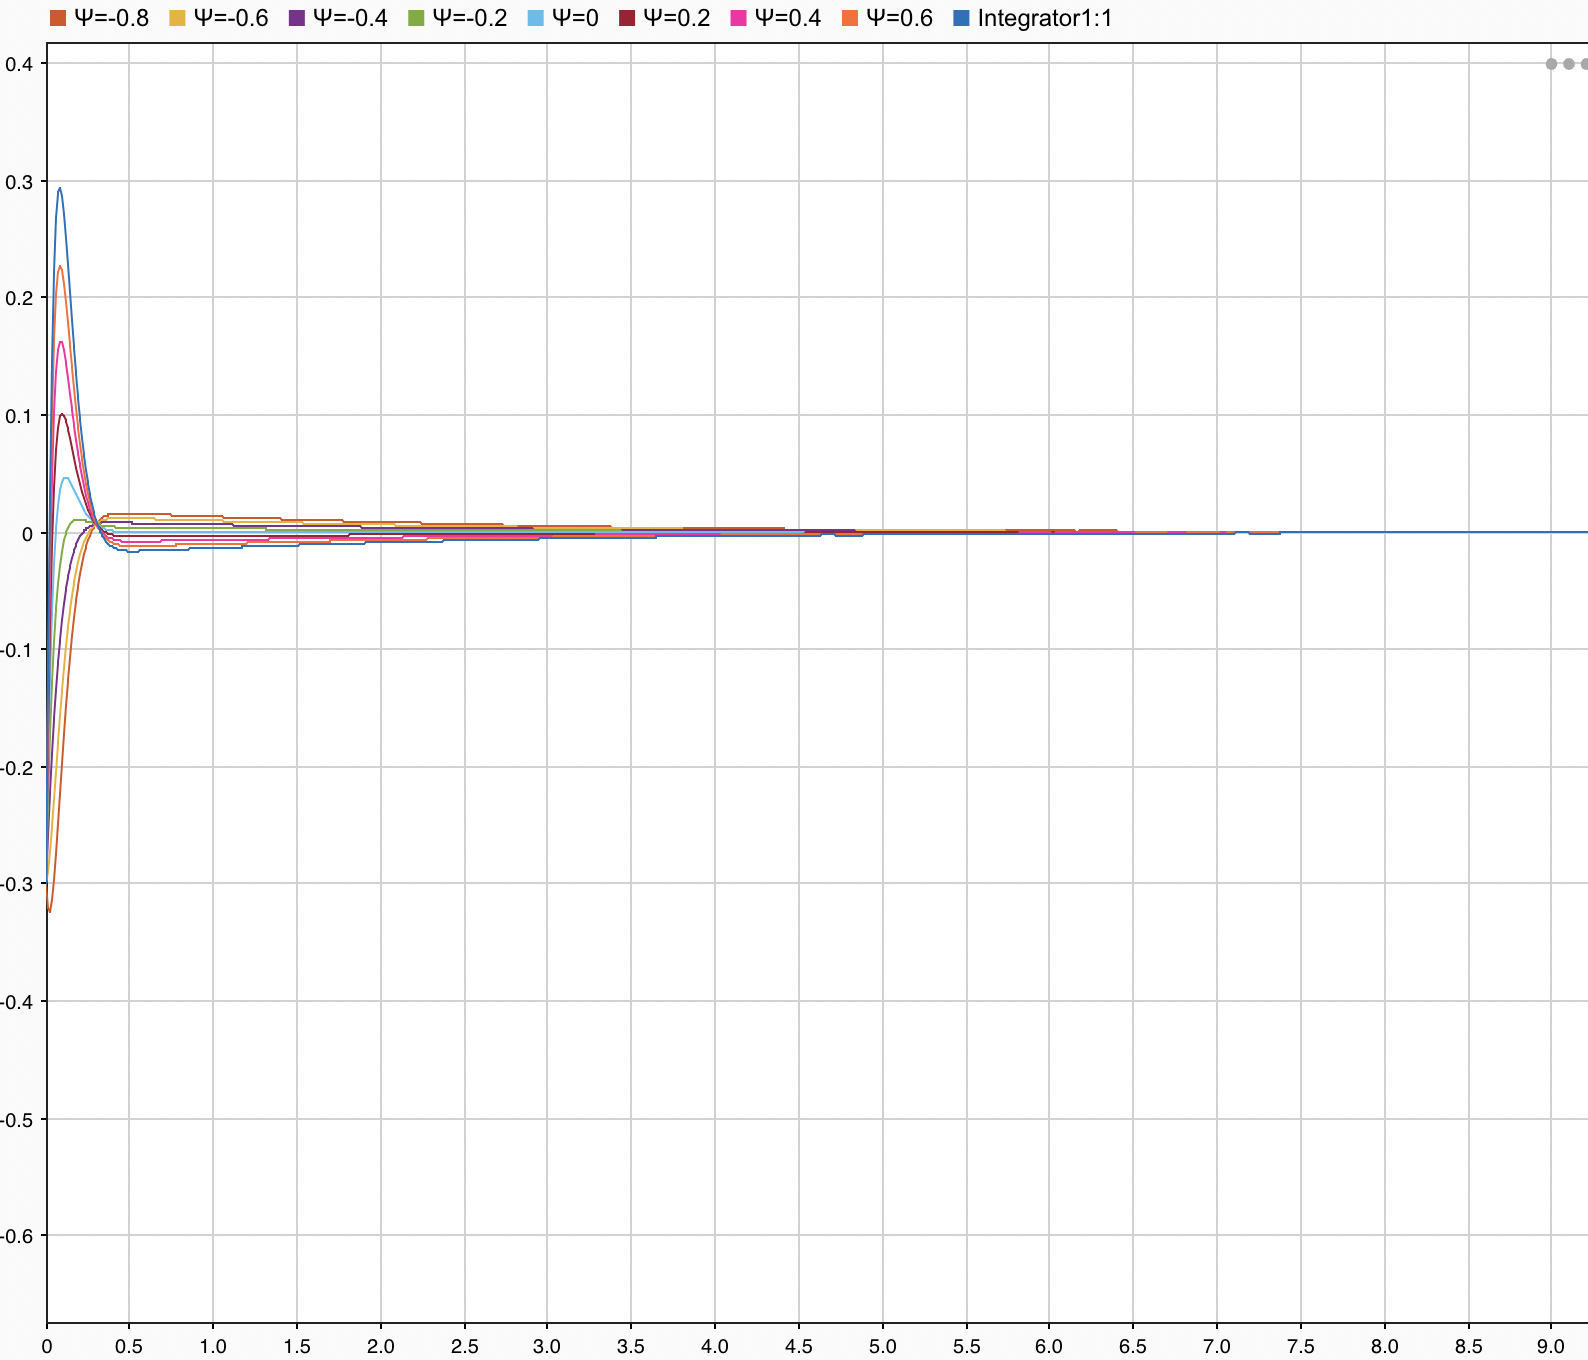
\includegraphics[width=\linewidth]{img8.png}
      \caption{Plots for y=-0.3}
    \end{subfigure}
    \begin{subfigure}{0.4\linewidth}
        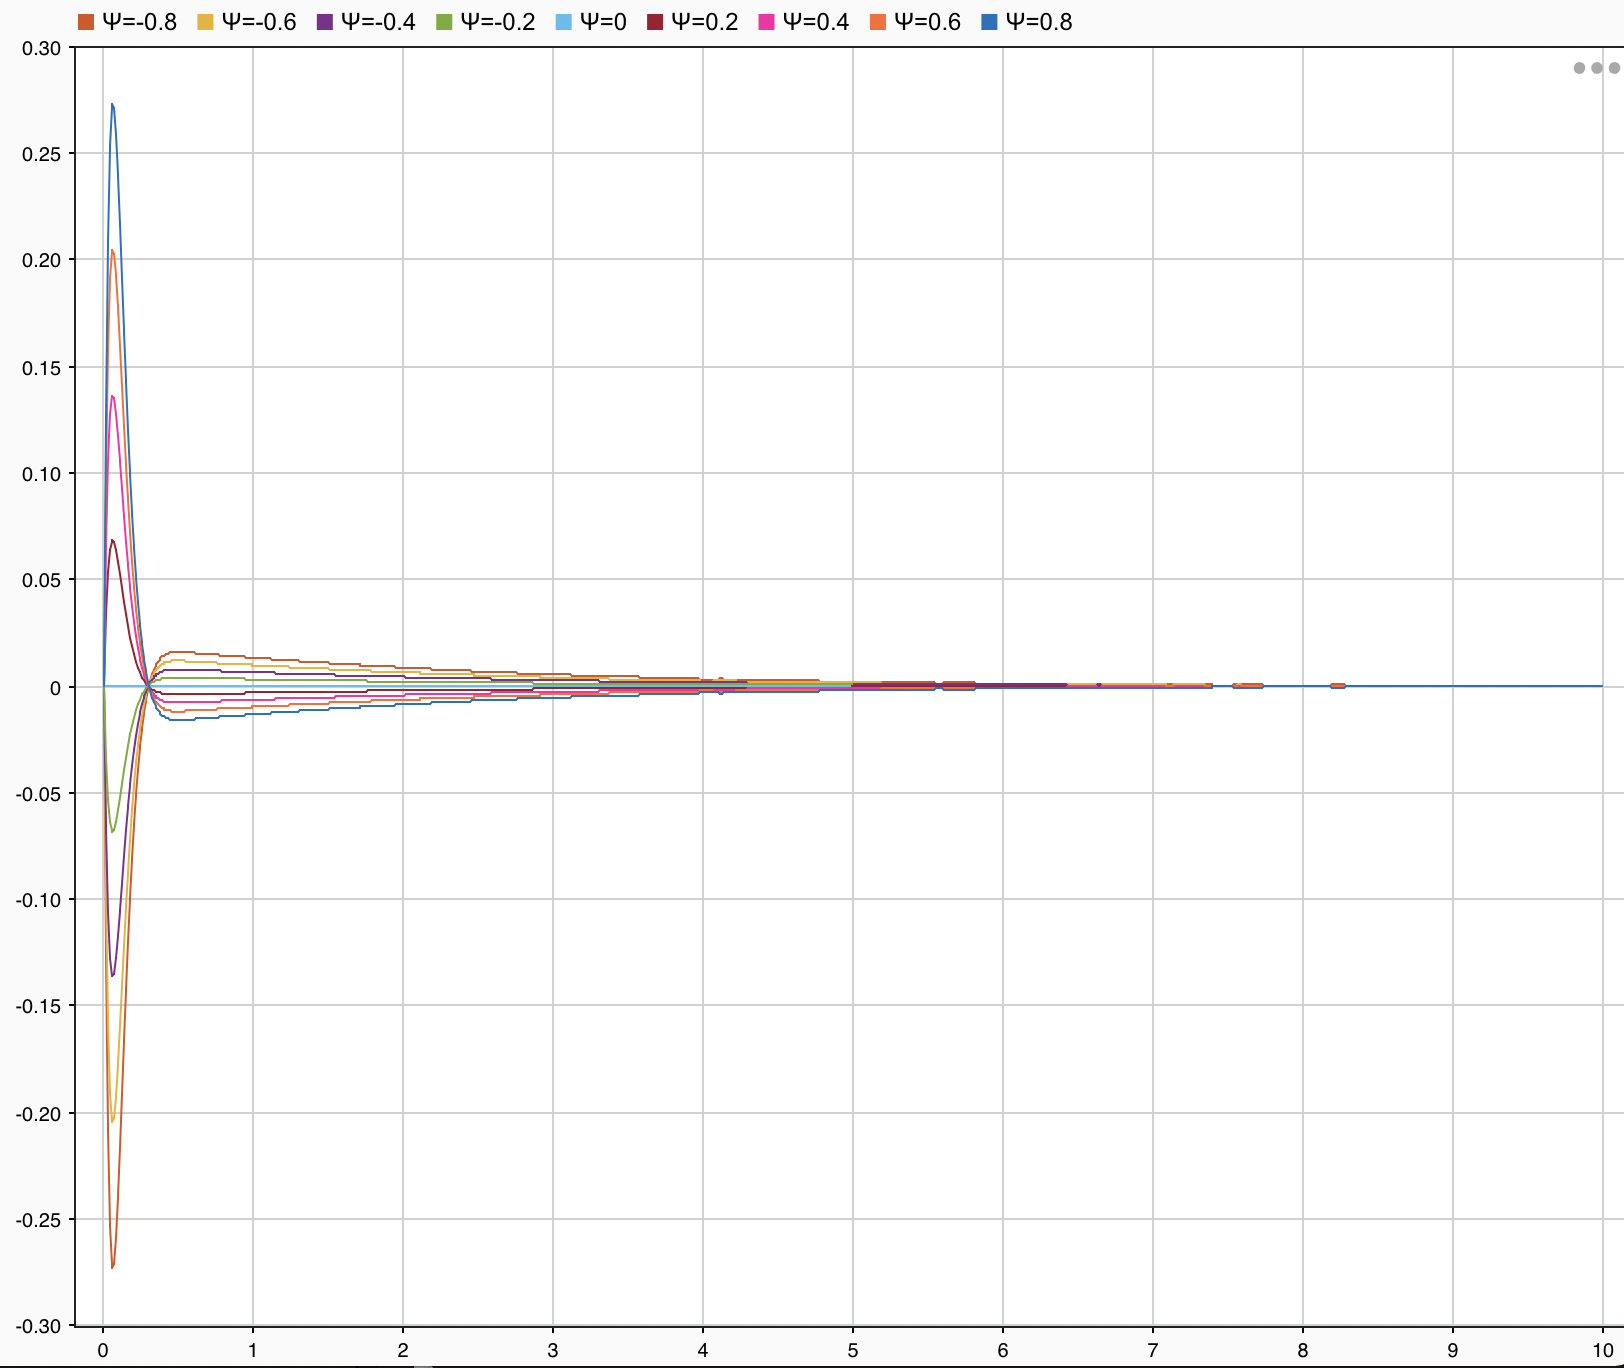
\includegraphics[width=\linewidth]{img9.png}
        \caption{Plots for y=-0}
      \end{subfigure}
      \begin{subfigure}{0.4\linewidth}
        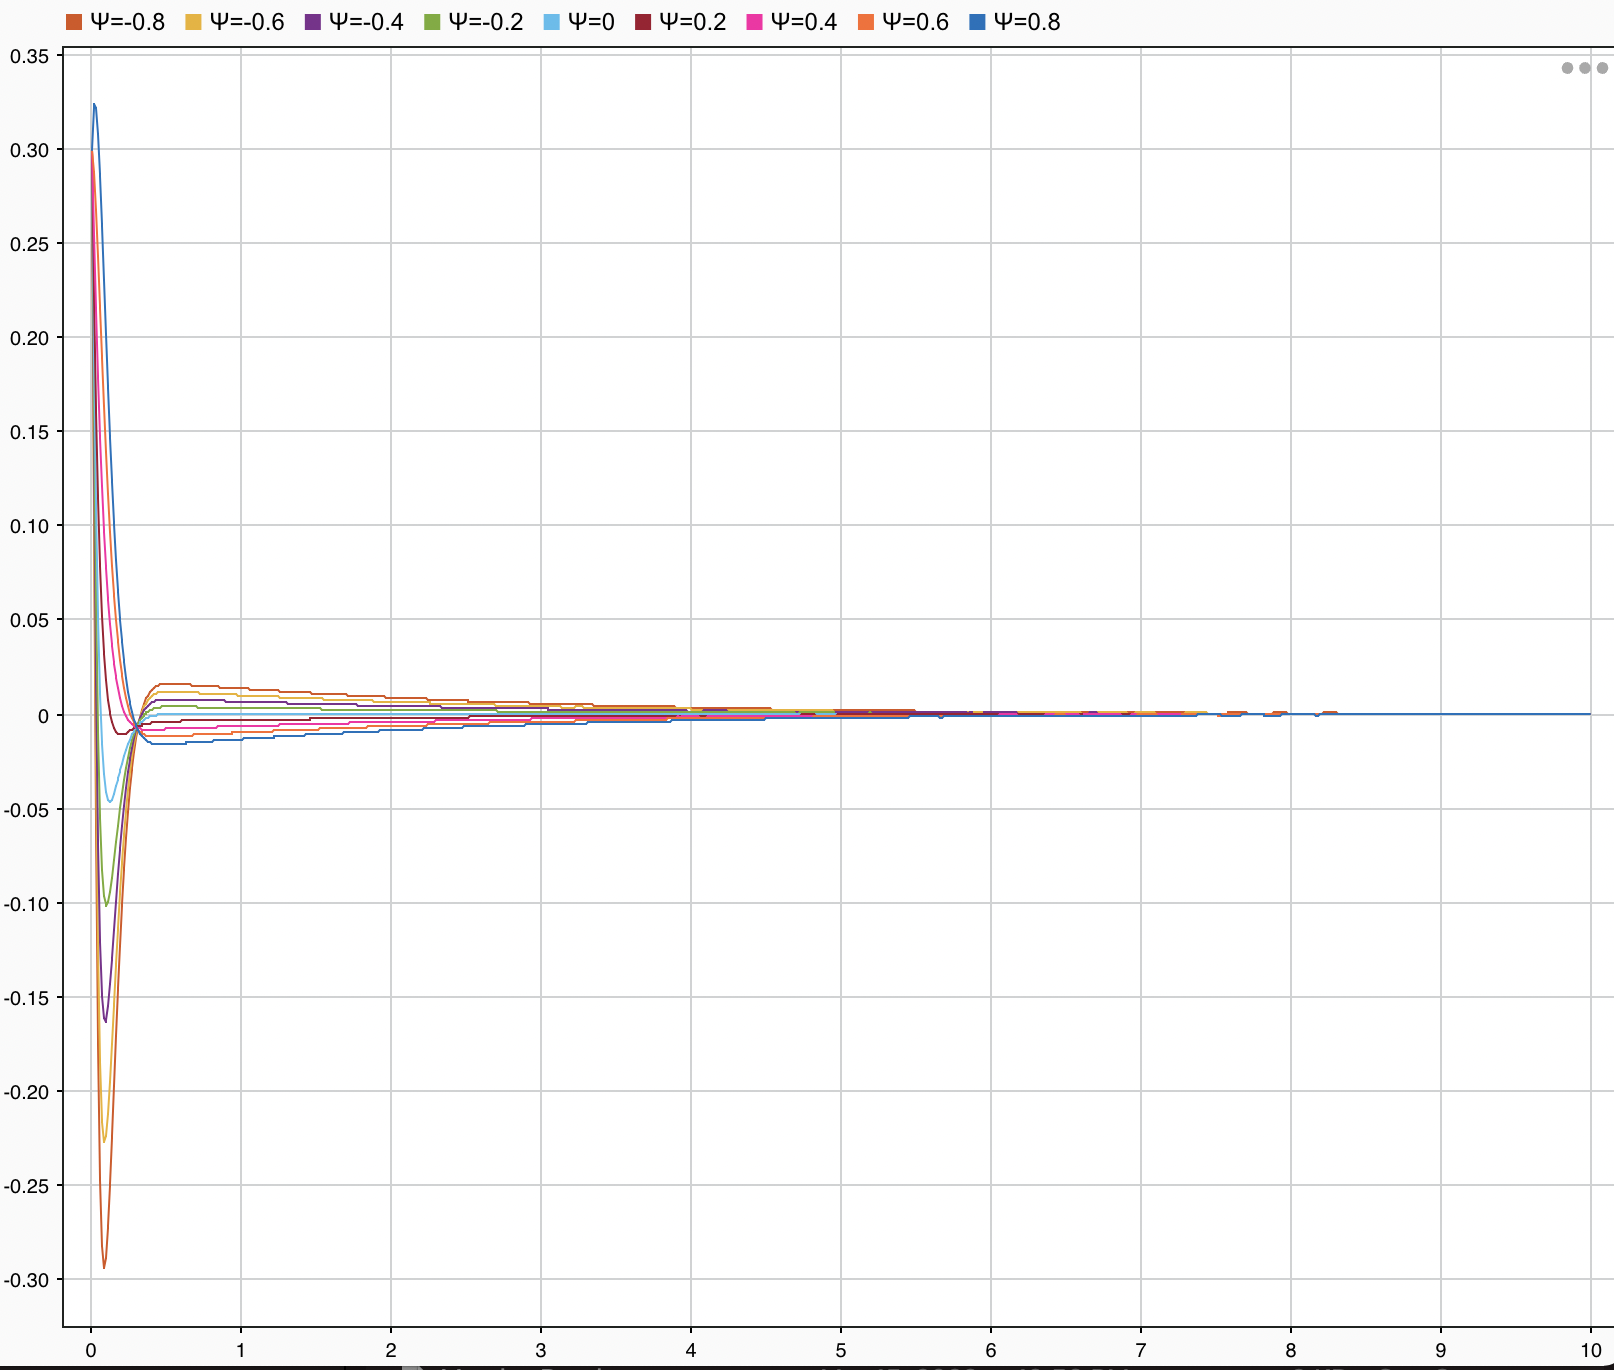
\includegraphics[width=\linewidth]{img10.png}
        \caption{Plots for y=0.3}
      \end{subfigure}
      \begin{subfigure}{0.4\linewidth}
          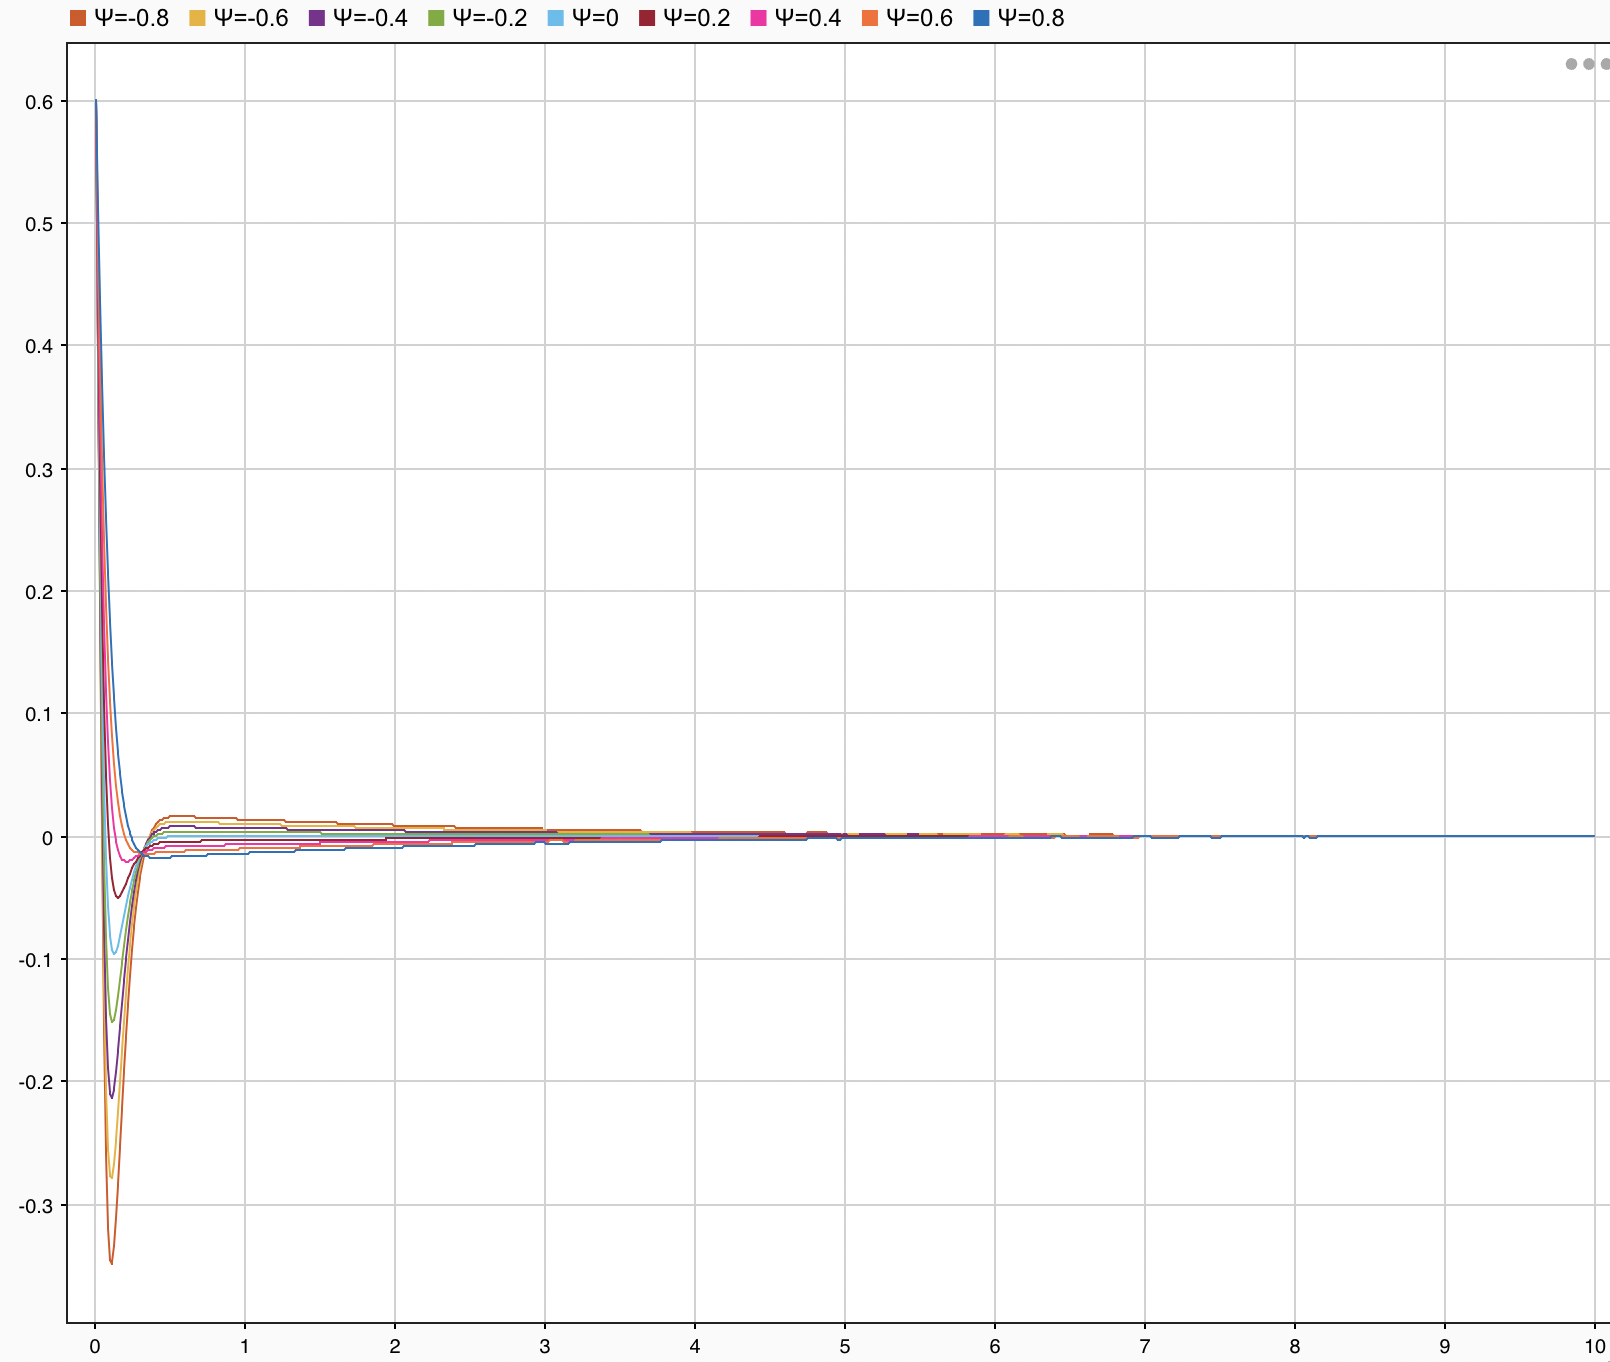
\includegraphics[width=\linewidth]{img11.png}
          \caption{Plots for y=0.6}
        \end{subfigure}
    \caption{Plots for different initial conditions}

  \end{figure}

\end{proof}

\newpage

\subsection*{Problem 4}
We now consider the velocity regulation problem. For this purpose we assume that
$y = 0$. Linearize the equations of motion to obtain the transfer function from $a$ to $v$ and
design a controller so that the closed-loop system tracks step inputs with zero steady-
state error. You don’t need to work with equation (1) since $x$ will not be at equilibrium.
Provide some plots showing the controller works as intended.

\begin{proof}[Solution]
First, we note that our given differential equation is $\dot{v}=a$, and taking the laplace gives us $\frac{v(s)}{a(s)}=\frac{1}{s}$.
Note that this makes sense as integrating $a$ gives us $v$. \newline
Now, we can implement a simple PID controller. With unit feedback, our transfer function with the controller is:
\[\dfrac{\frac{s^2k_{D}+sk_{P}+k_{I}}{s^2}}{1+\frac{s^2k_{D}+sk_{P}+k_{I}}{s^2}}
\]
Thus, on the denominator, we have: 
\[s^2(1+k_{D})+k_{P}s+k_{I}=0
\]
\[s^2+\frac{k_{P}}{1+k_{D}}s+\frac{k_{I}}{1+k_{D}}
\]
Now, let us try to find PID constants such that the system is critically damped, or when $\zeta=1$.
Then, we have that:
\[\omega_{n} = \sqrt{\frac{k_{I}}{1+k_{D}}}\]
\[2\omega_{n}=\frac{k_{P}}{1+k_{D}}\]
\[\frac{k_{P}}{2+2k_{D}} =  \sqrt{\frac{k_{I}}{1+k_{D}}}\]
Here, we can pick $k_P=2$,$k_D=1$, and $k_I=\frac{1}{2}$ to satisfy this equation. 

\begin{figure}[h!]
    \centering
    \begin{subfigure}{0.4\linewidth}
      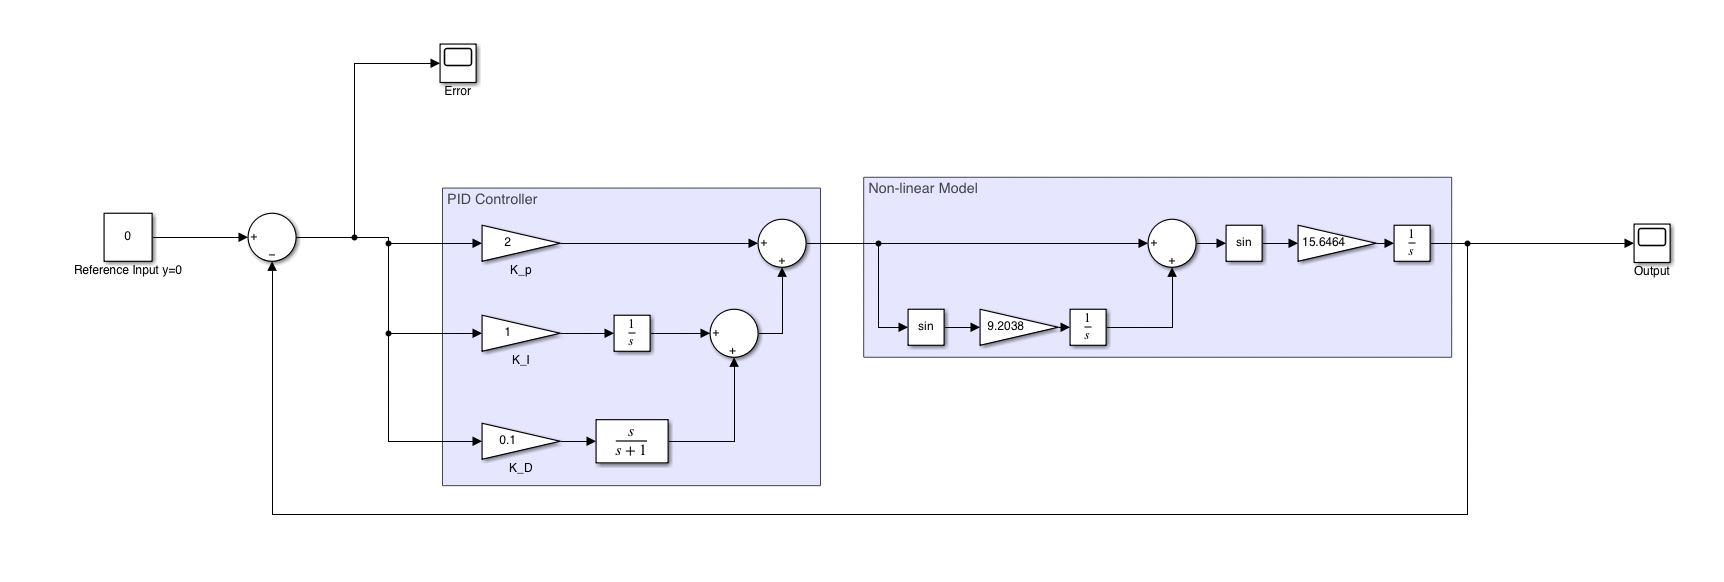
\includegraphics[width=\linewidth]{Q3Model.png}
      \caption{Simulink Block Diagram from PID velocity Model}
    \end{subfigure}
    \begin{subfigure}{0.4\linewidth}
      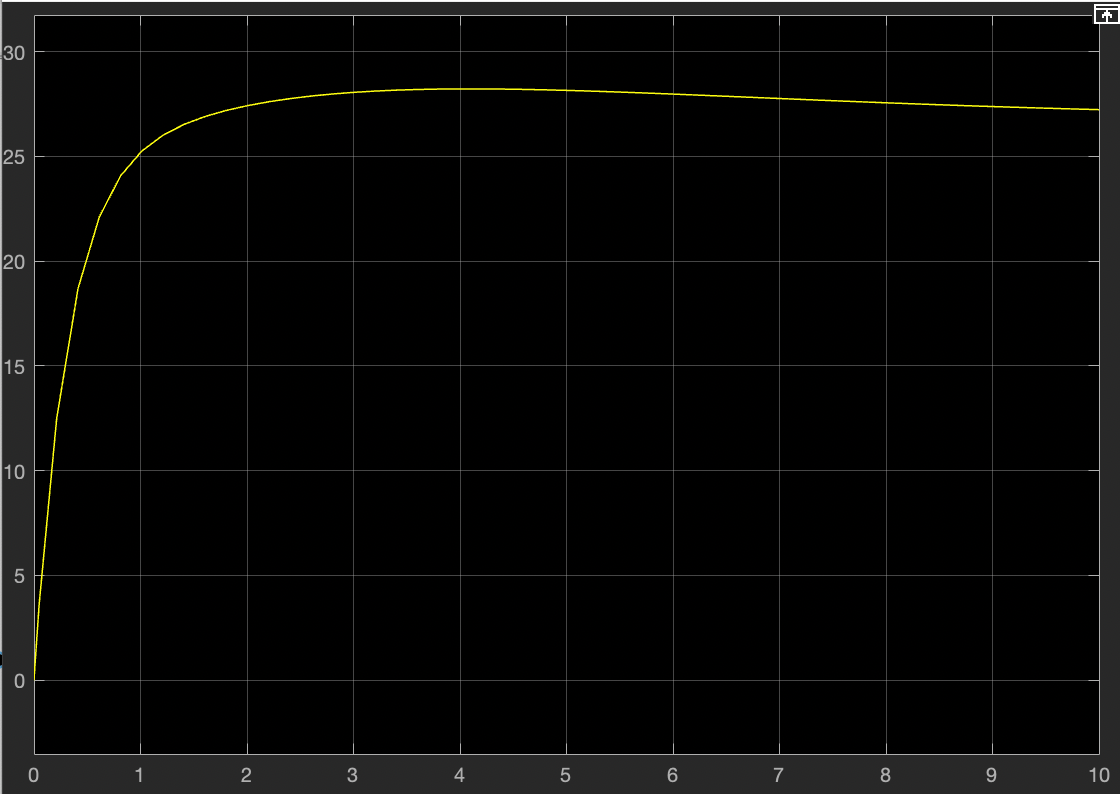
\includegraphics[width=\linewidth]{img12.png}
      \caption{Step Response modeling time to reach 60mph for PID model}
    \end{subfigure}
    \caption{Plots for Original PID Control}
  \end{figure}

A normal time for fast cars to take to reach 60 mph, which is 26.8224 m/s is around 5 seconds, so let us assume maximum acceleration is somewhere around $26.8224/5 \approx 5.4$.
Our car is therefore accelerating abnormally fast. To solve this issue, let us cap our accleration with a saturation block at 5.4 m/s/s.
As such, even though there is overshoot, the acceleration is more normal, and is about in line with modern sports cars.

  \begin{figure}[h!]
    \centering
    \begin{subfigure}{0.4\linewidth}
      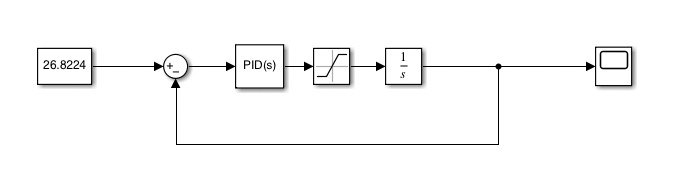
\includegraphics[width=\linewidth]{q3goodmodel.png}
      \caption{Simulink Block Diagram from PID with Saturation Block velocity model}
    \end{subfigure}
    \begin{subfigure}{0.4\linewidth}
      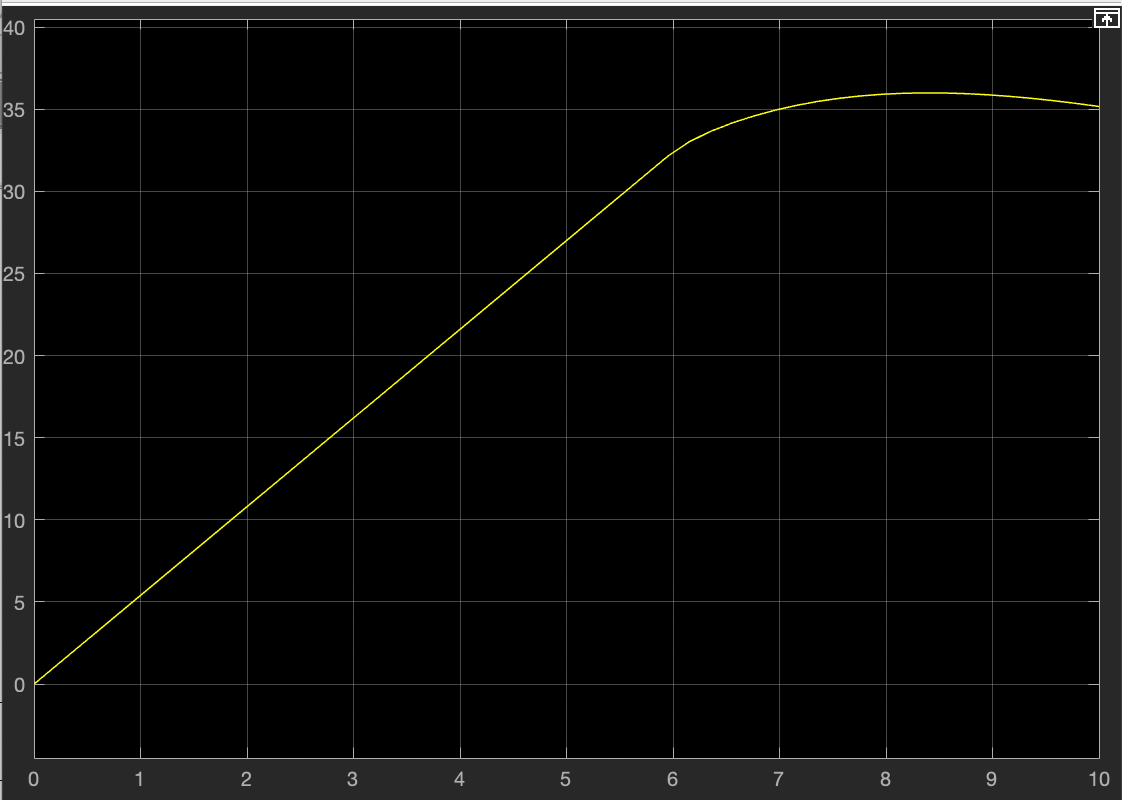
\includegraphics[width=\linewidth]{img13.png}
      \caption{Step Response modeling time to reach 60mph for PID with Saturation model}
    \end{subfigure}
    \caption{Plots for PID with Saturation block}
  \end{figure}

  We can confirm that this model works for 
\end{proof}

\newpage
\subsection*{Problem 5}
Simulate the nonlinear car model in closed-loop with both controllers. Note the assump-
tions made when designing the controllers are no longer satisfied: velocity is no longer
constant and $y$ no longer equals zero. Find the range of initial conditions for which
the designed controllers have adequate performance when the commanded velocity is 35
mph. What happens when the controller regulating velocity is much slower than the
controller regulating the position in the lane? Provide some plots to justify your answer.

\begin{proof}[Solution]
We begin by creating the simulink model:
\begin{figure}[h!]
    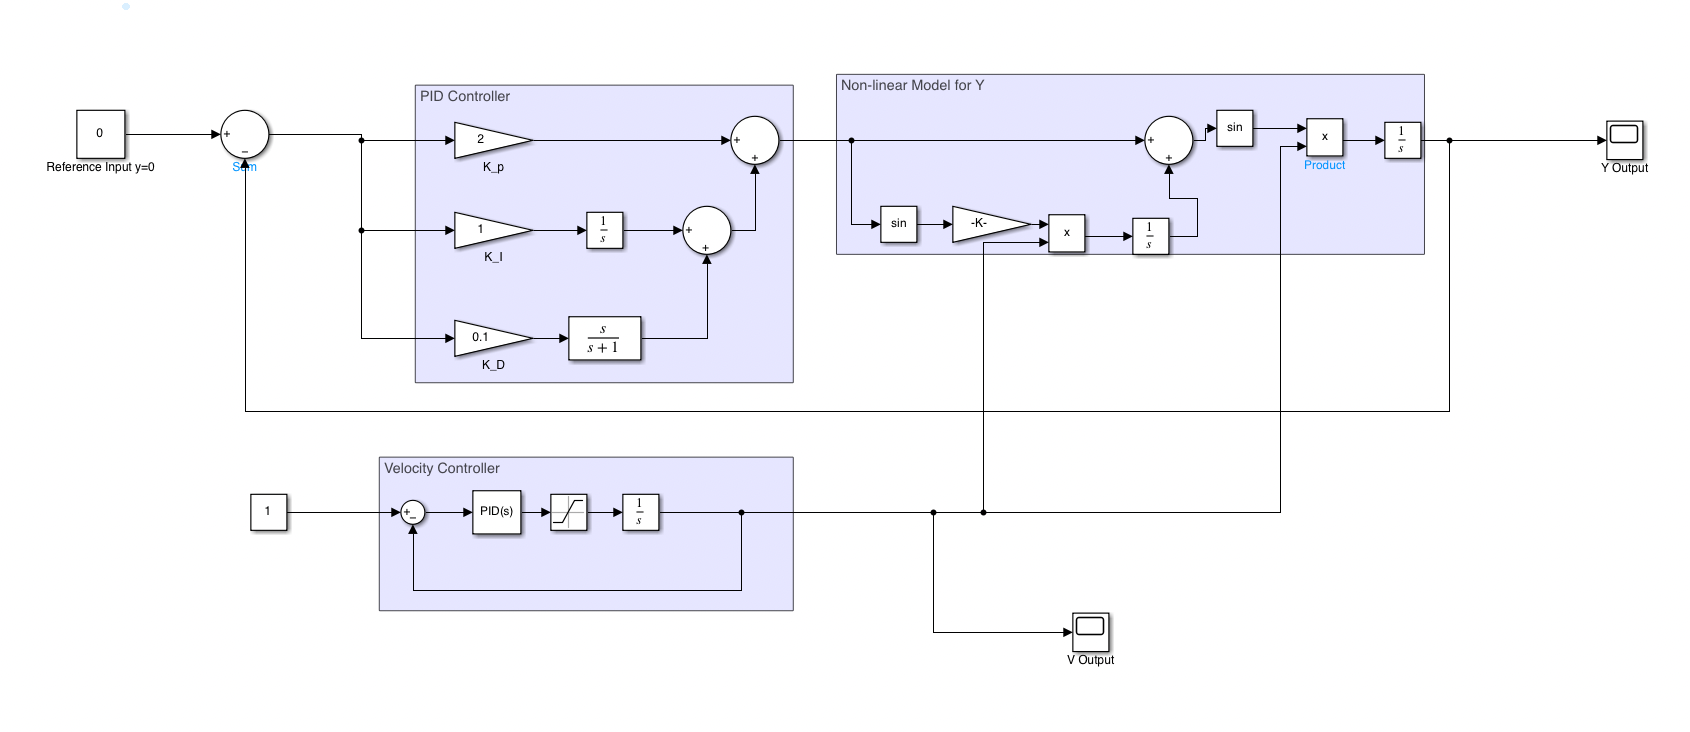
\includegraphics[width=\linewidth]{q5model.png}
    \caption{Simulink Model for Velocity and Position Controllers}
\end{figure}

Note that in this case, the controller regulating velocity is much slower than the controller regulating position due to our saturation block. 
We see from the figures below that the controller is acceptable although rising time is higher than the controller from Question 1.
Note the oscillations are not significant as none of them are above 0.2 m, a negligible amount. However, when the inital speed reaches
70 mph, or perhaps even earlier, the change in position is far more jerky and sudden. This is associated with rapid deceleration due to pressing of the breaks.
At 55.5 mph, the rising time is a little higher than 0.2s, so the maximum starting speed the controller can account for is 70mph.
Therefore, we've arrived at the following range of inital conditions
\[ v \in (0, 24.81) 
\]
\[ y \in (-0.6, 0.6)
\]
\begin{figure}[h!]
    \centering
    \begin{subfigure}{0.4\linewidth}
      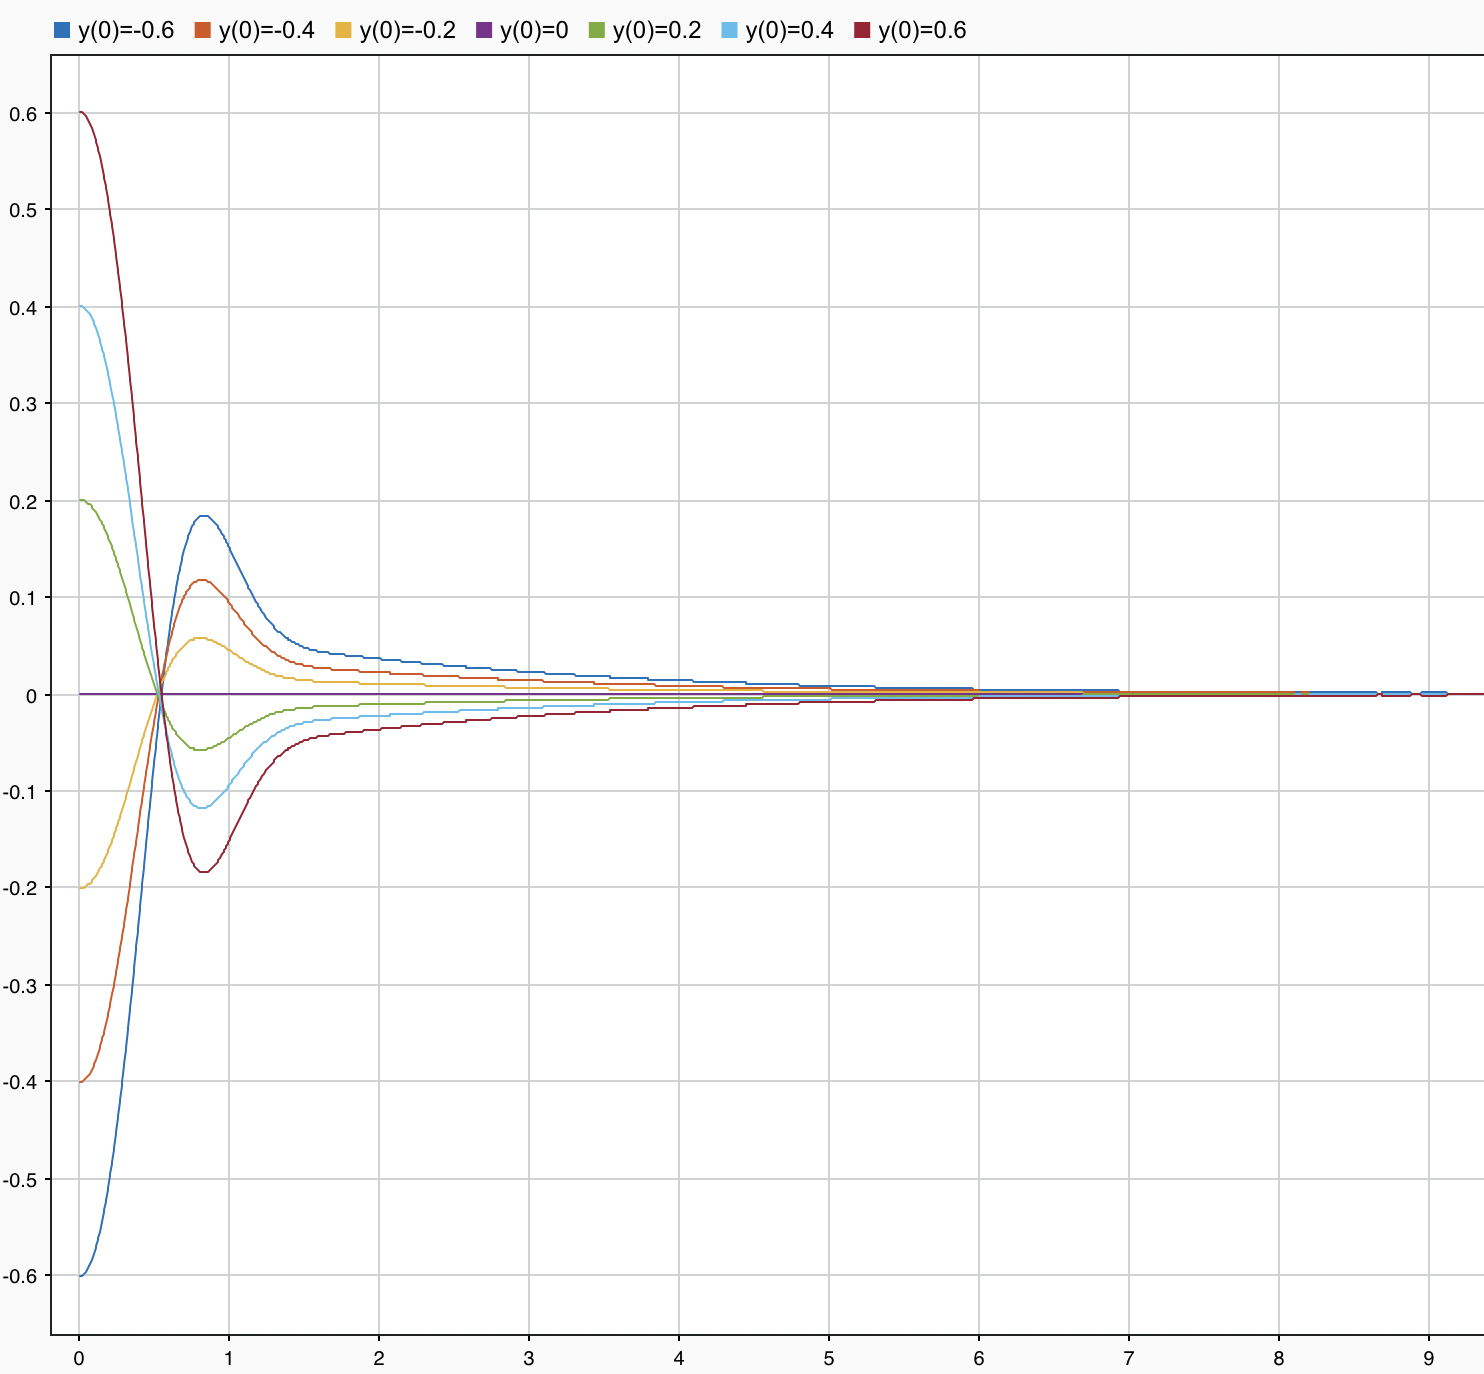
\includegraphics[width=\linewidth]{img14.png}
      \caption{Position}
    \end{subfigure}
    \begin{subfigure}{0.4\linewidth}
      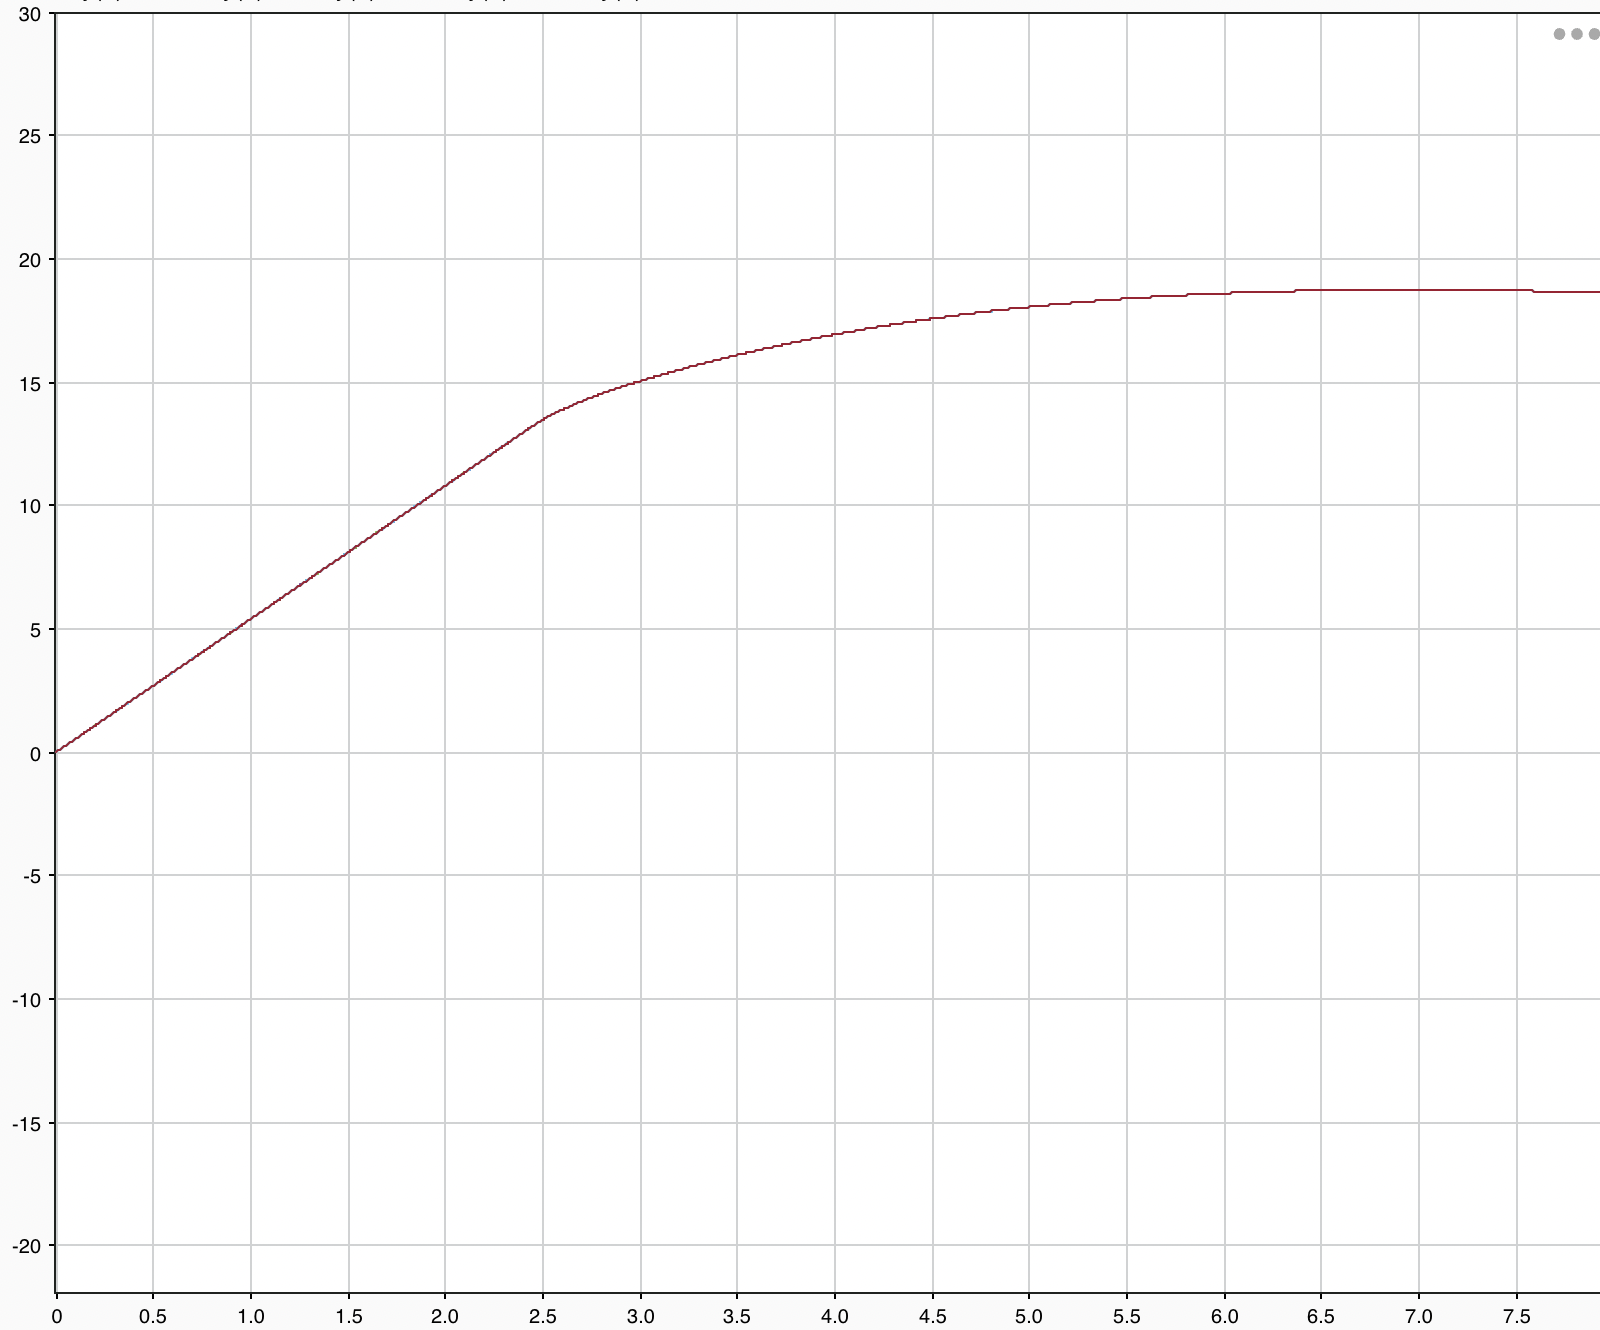
\includegraphics[width=\linewidth]{img15.png}
      \caption{Velocity}
    \end{subfigure}
    \caption{Plots for v(0)=0}
\end{figure}

  \begin{figure}[h!]
    \centering
    \begin{subfigure}{0.4\linewidth}
      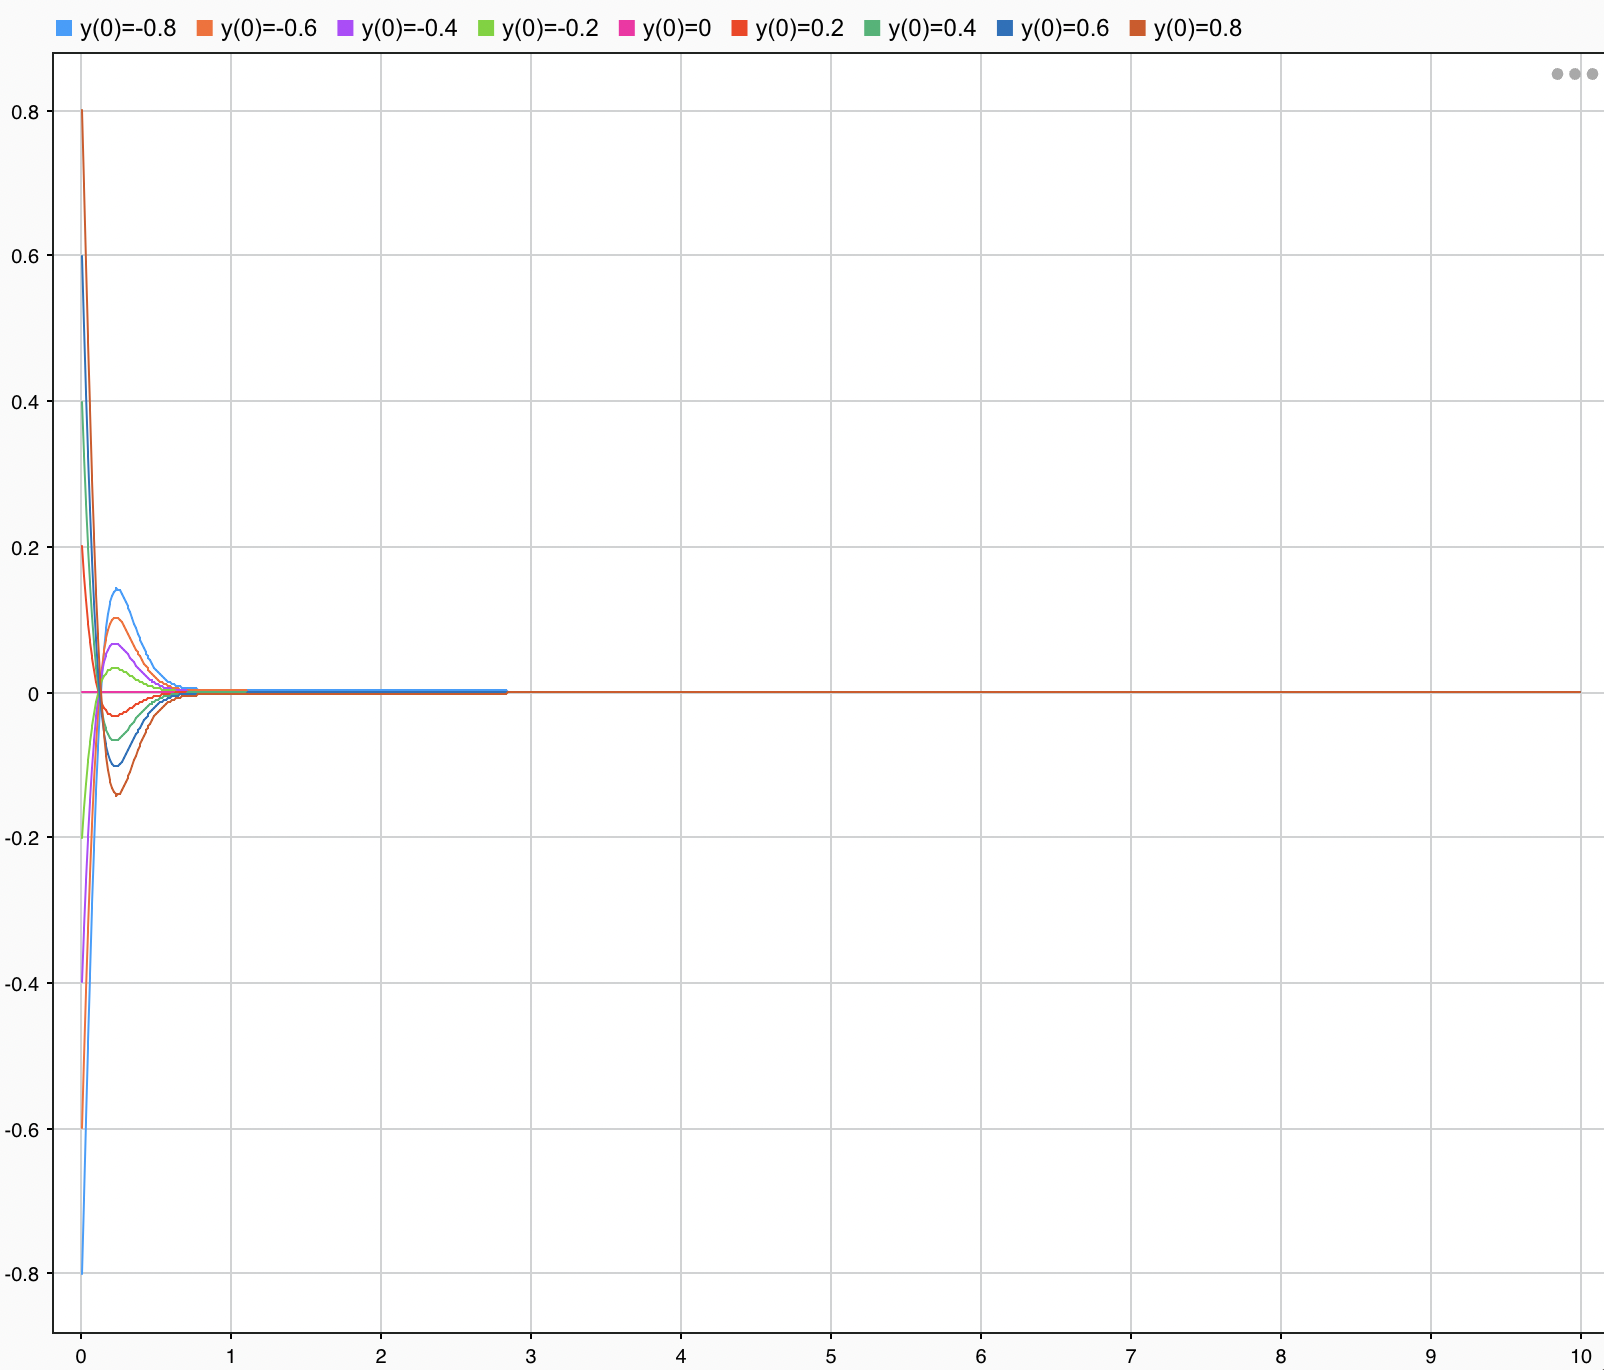
\includegraphics[width=\linewidth]{img16.png}
      \caption{Position}
    \end{subfigure}
    \begin{subfigure}{0.4\linewidth}
      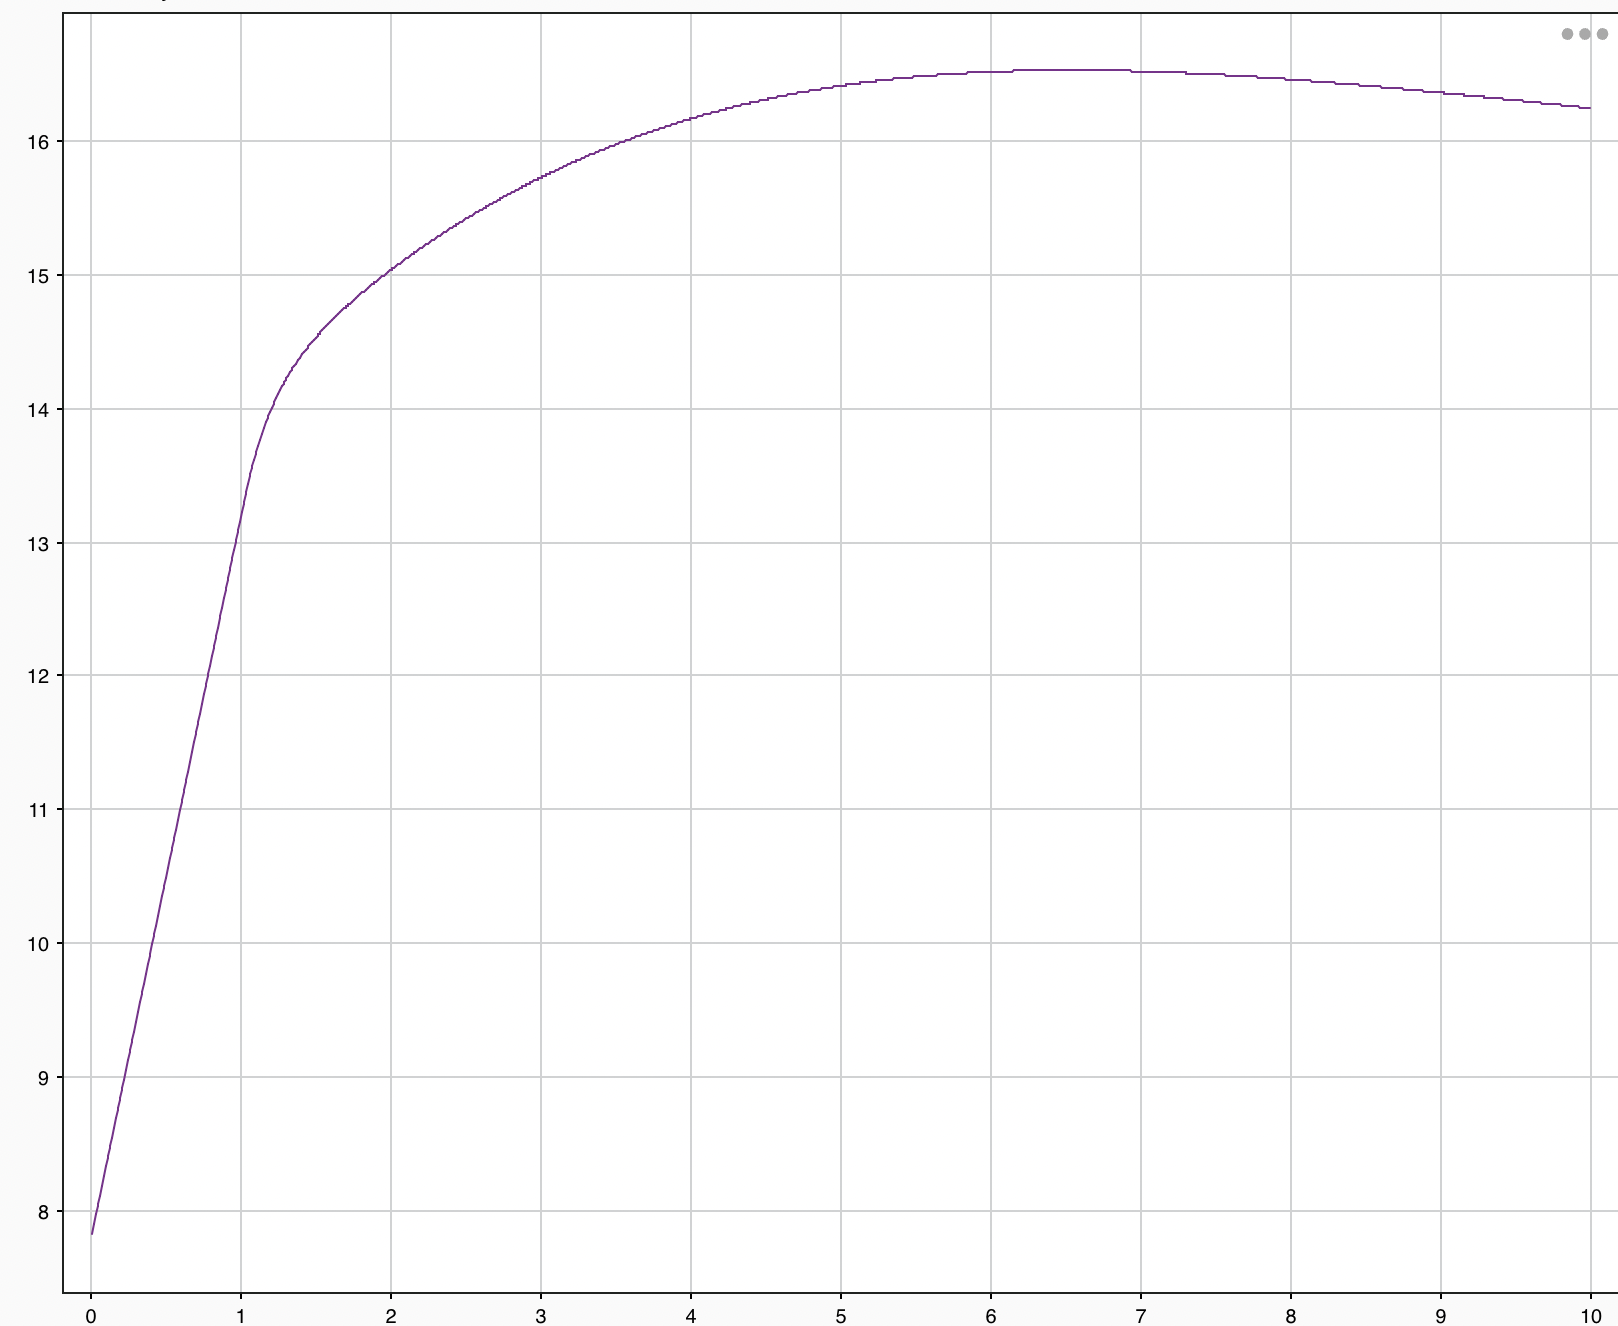
\includegraphics[width=\linewidth]{img17.png}
      \caption{Velocity}
    \end{subfigure}
    \caption{Plots for v(0)=35 mph}
  \end{figure}

  \begin{figure}[h!]
    \centering
    \begin{subfigure}{0.4\linewidth}
      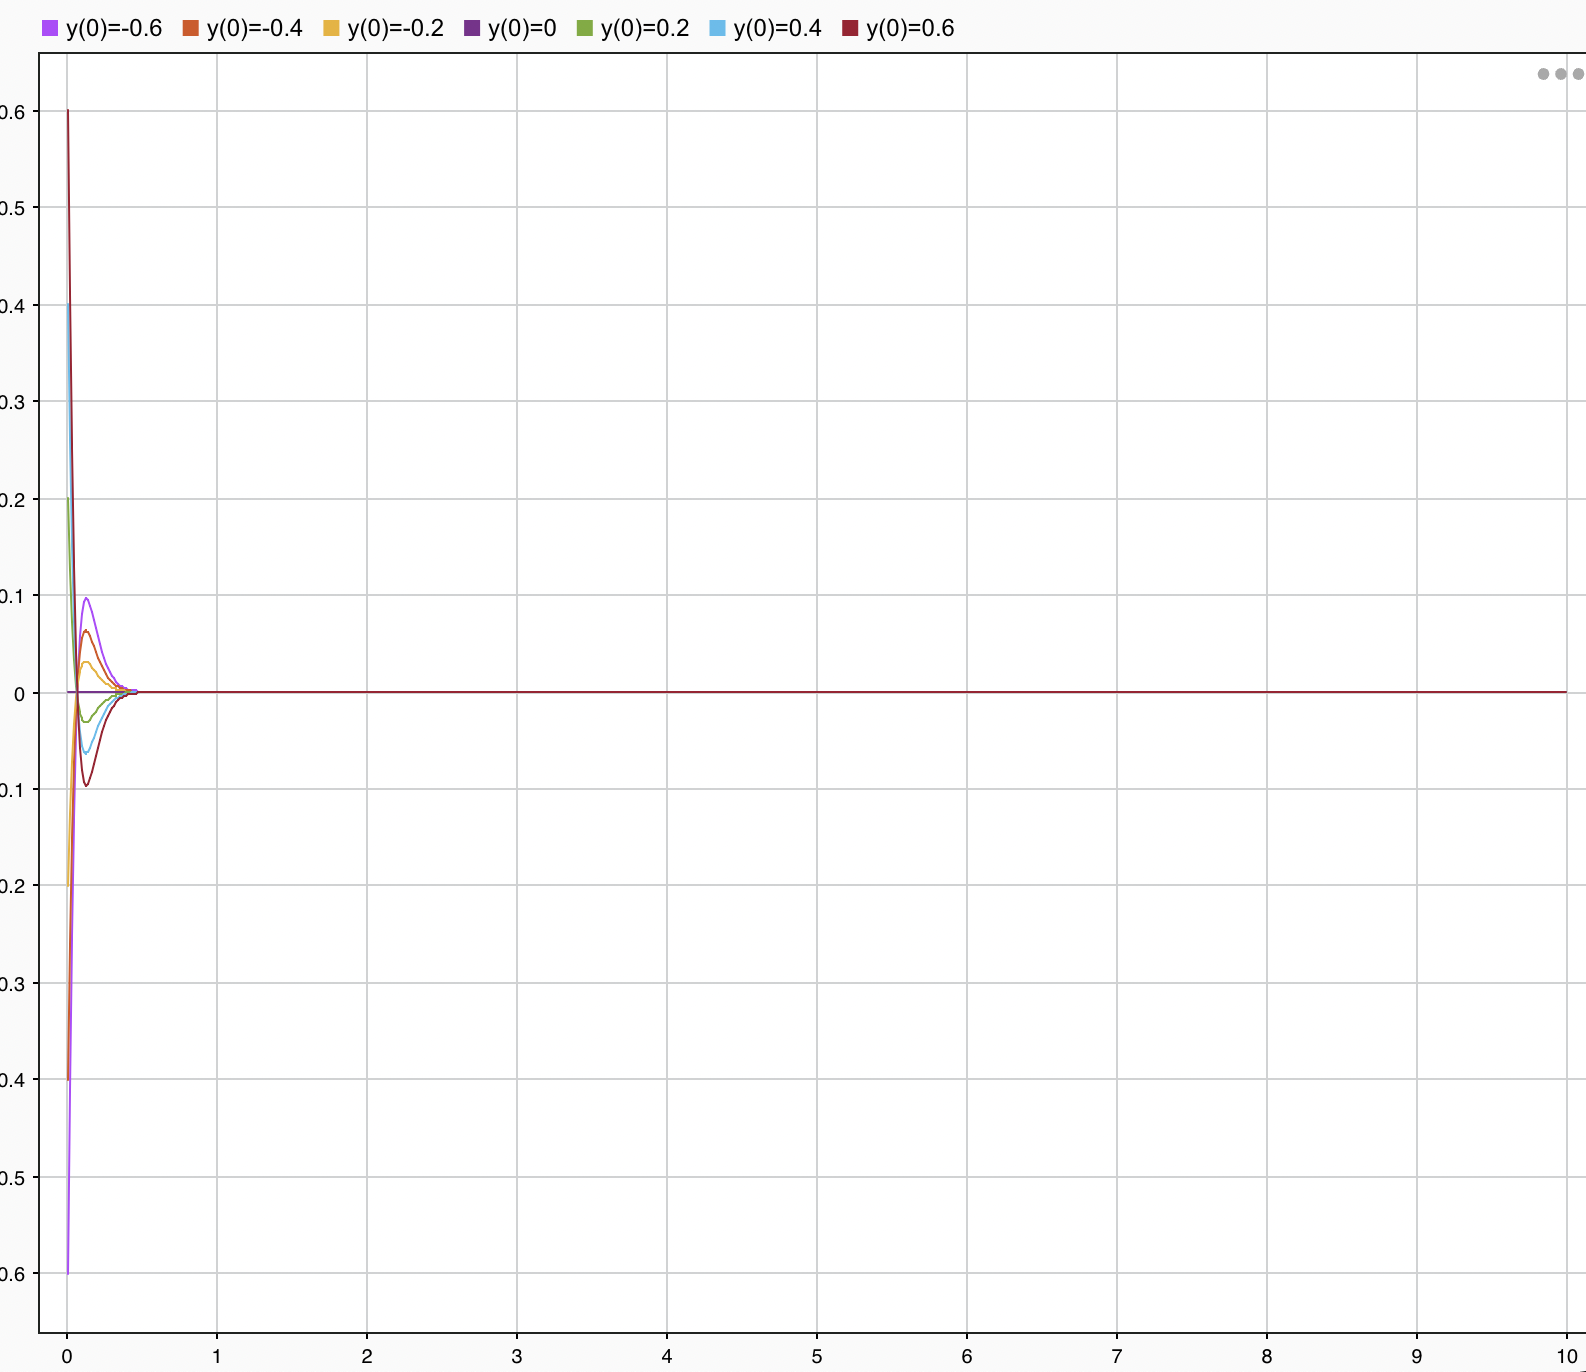
\includegraphics[width=\linewidth]{img18.png}
      \caption{Position}
    \end{subfigure}
    \begin{subfigure}{0.4\linewidth}
      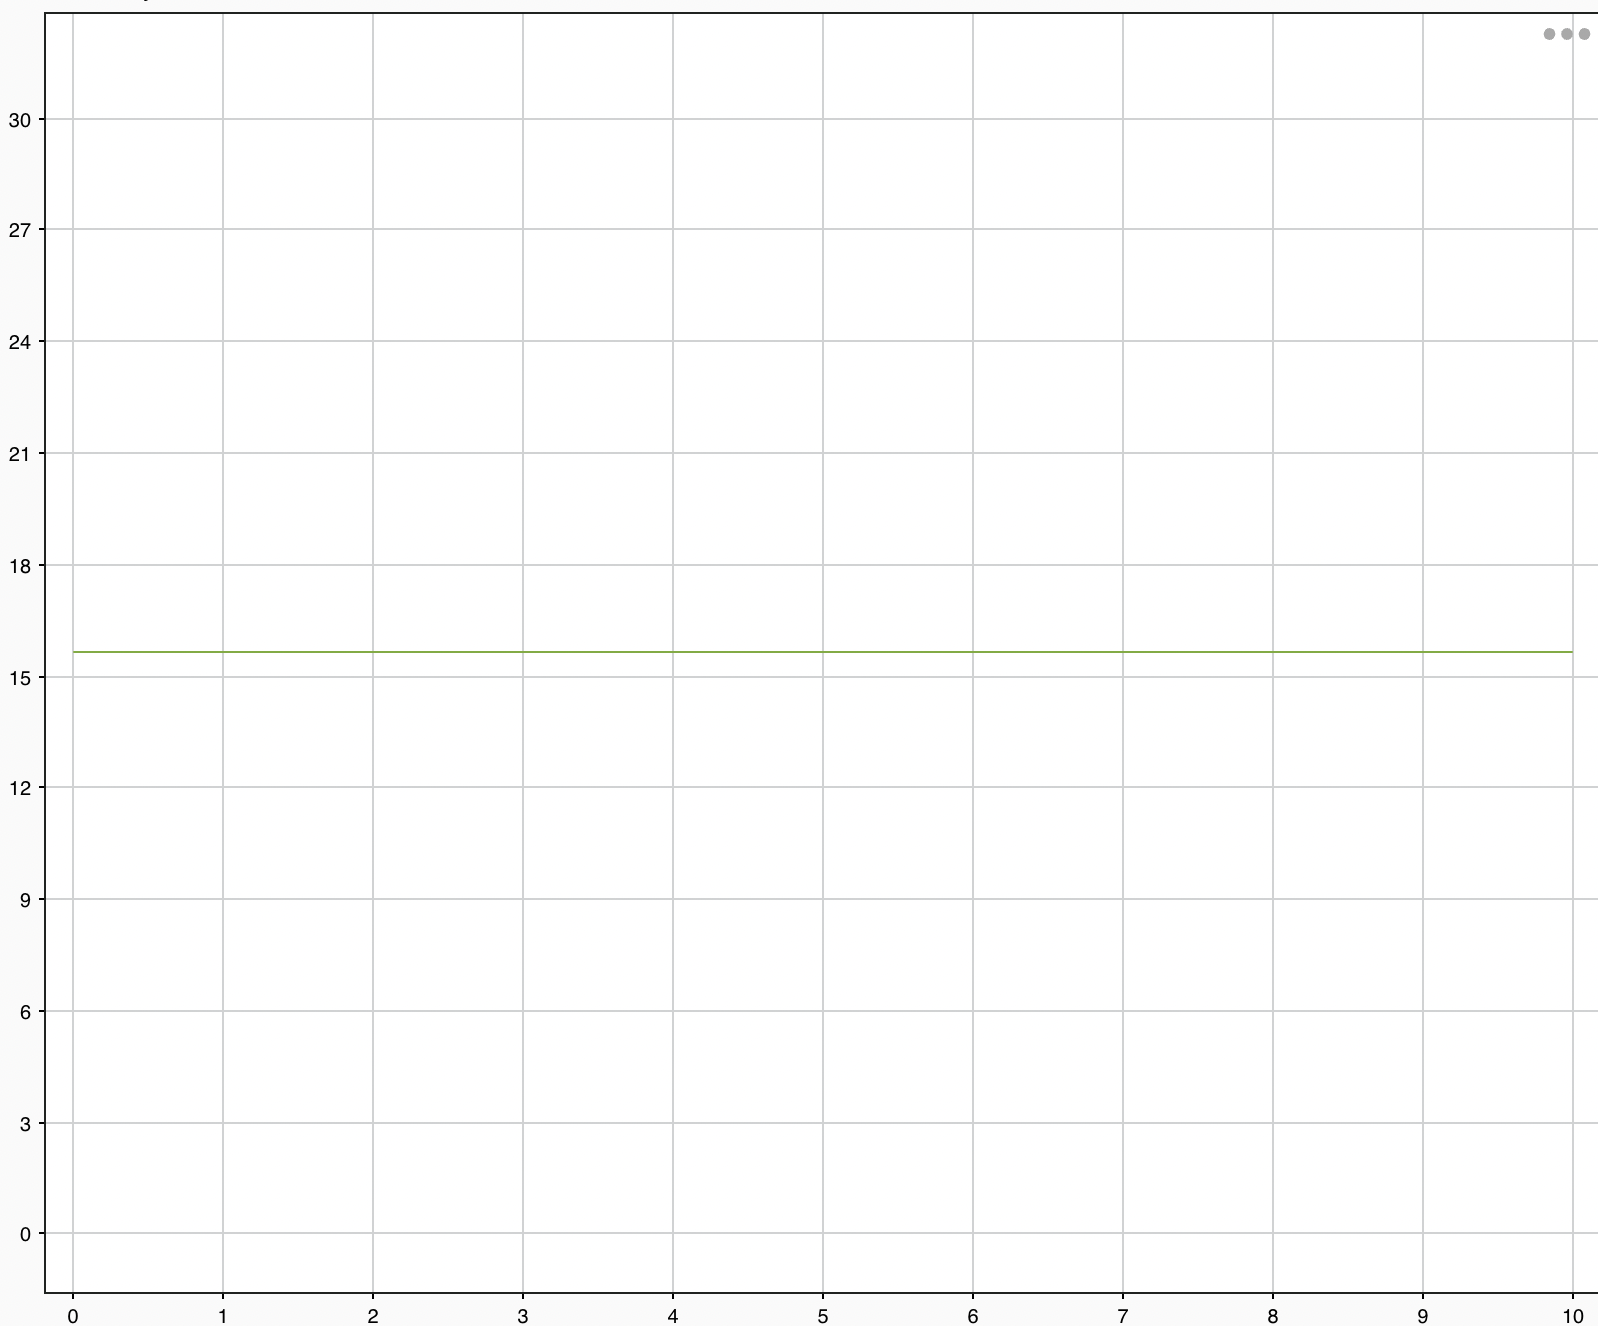
\includegraphics[width=\linewidth]{img19.png}
      \caption{Velocity}
    \end{subfigure}
    \caption{Plots for v(0)=35 mph}
  \end{figure}

  \begin{figure}[h!]
    \centering
    \begin{subfigure}{0.4\linewidth}
      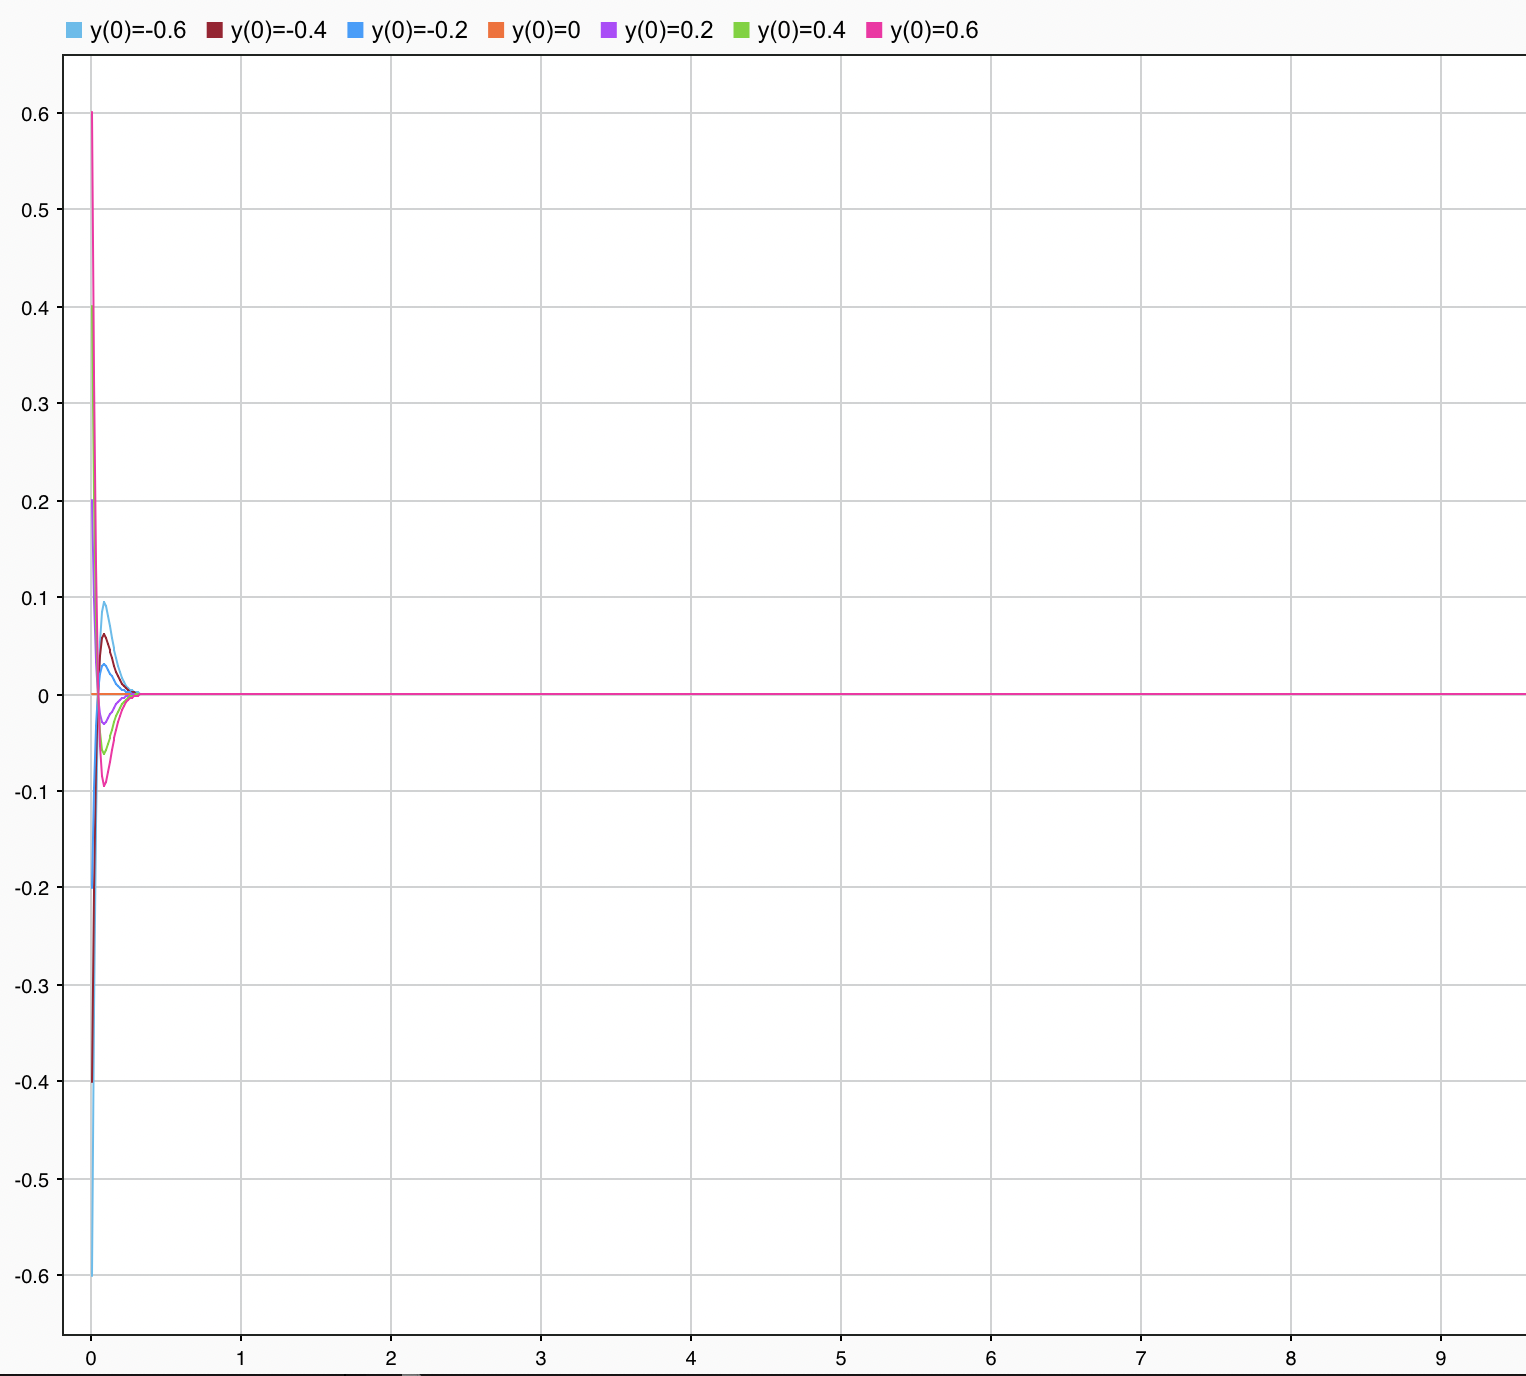
\includegraphics[width=\linewidth]{img20.png}
      \caption{Position}
    \end{subfigure}
    \begin{subfigure}{0.4\linewidth}
      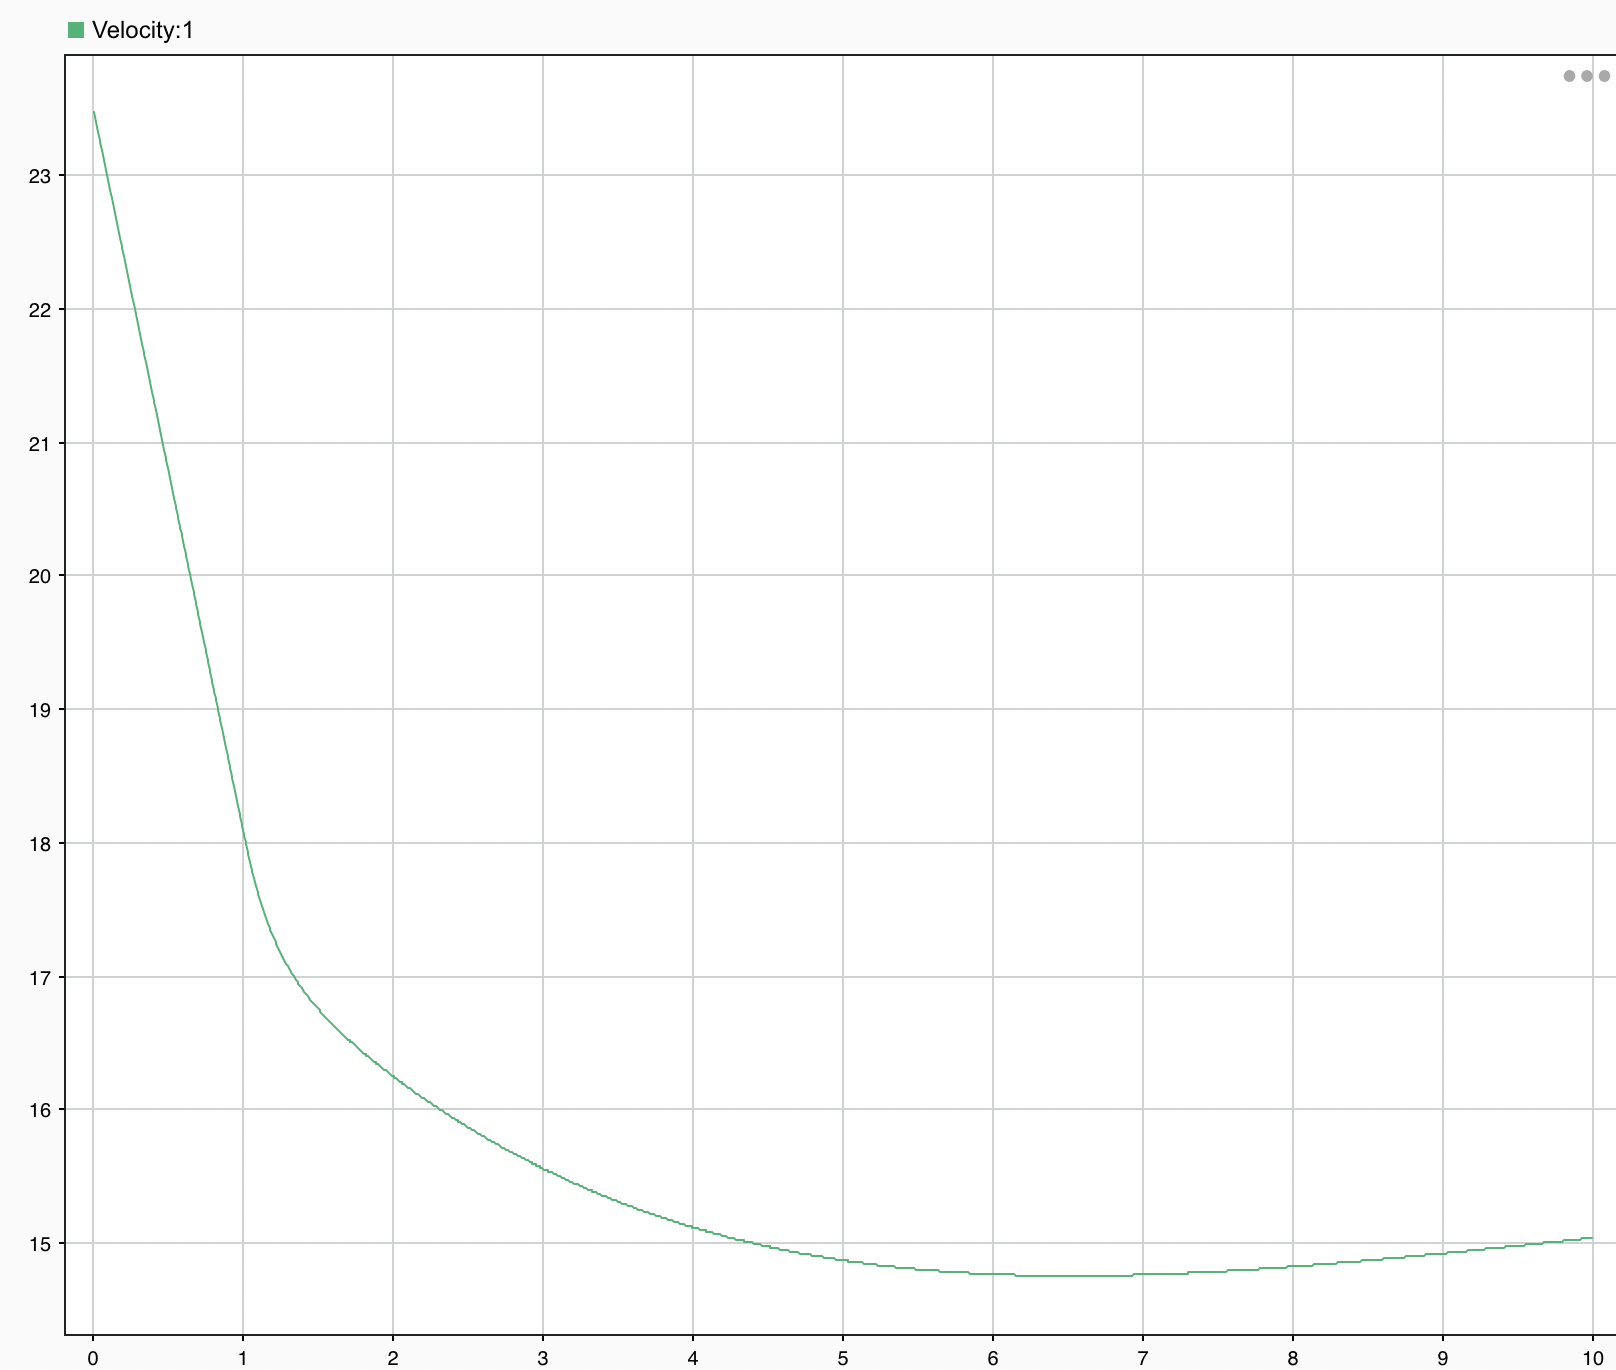
\includegraphics[width=\linewidth]{img21.png}
      \caption{Velocity}
    \end{subfigure}
    \caption{Plots for v(0)=52.5 mph}
\end{figure}

    \begin{figure}[h!]
        \centering
        \begin{subfigure}{0.4\linewidth}
          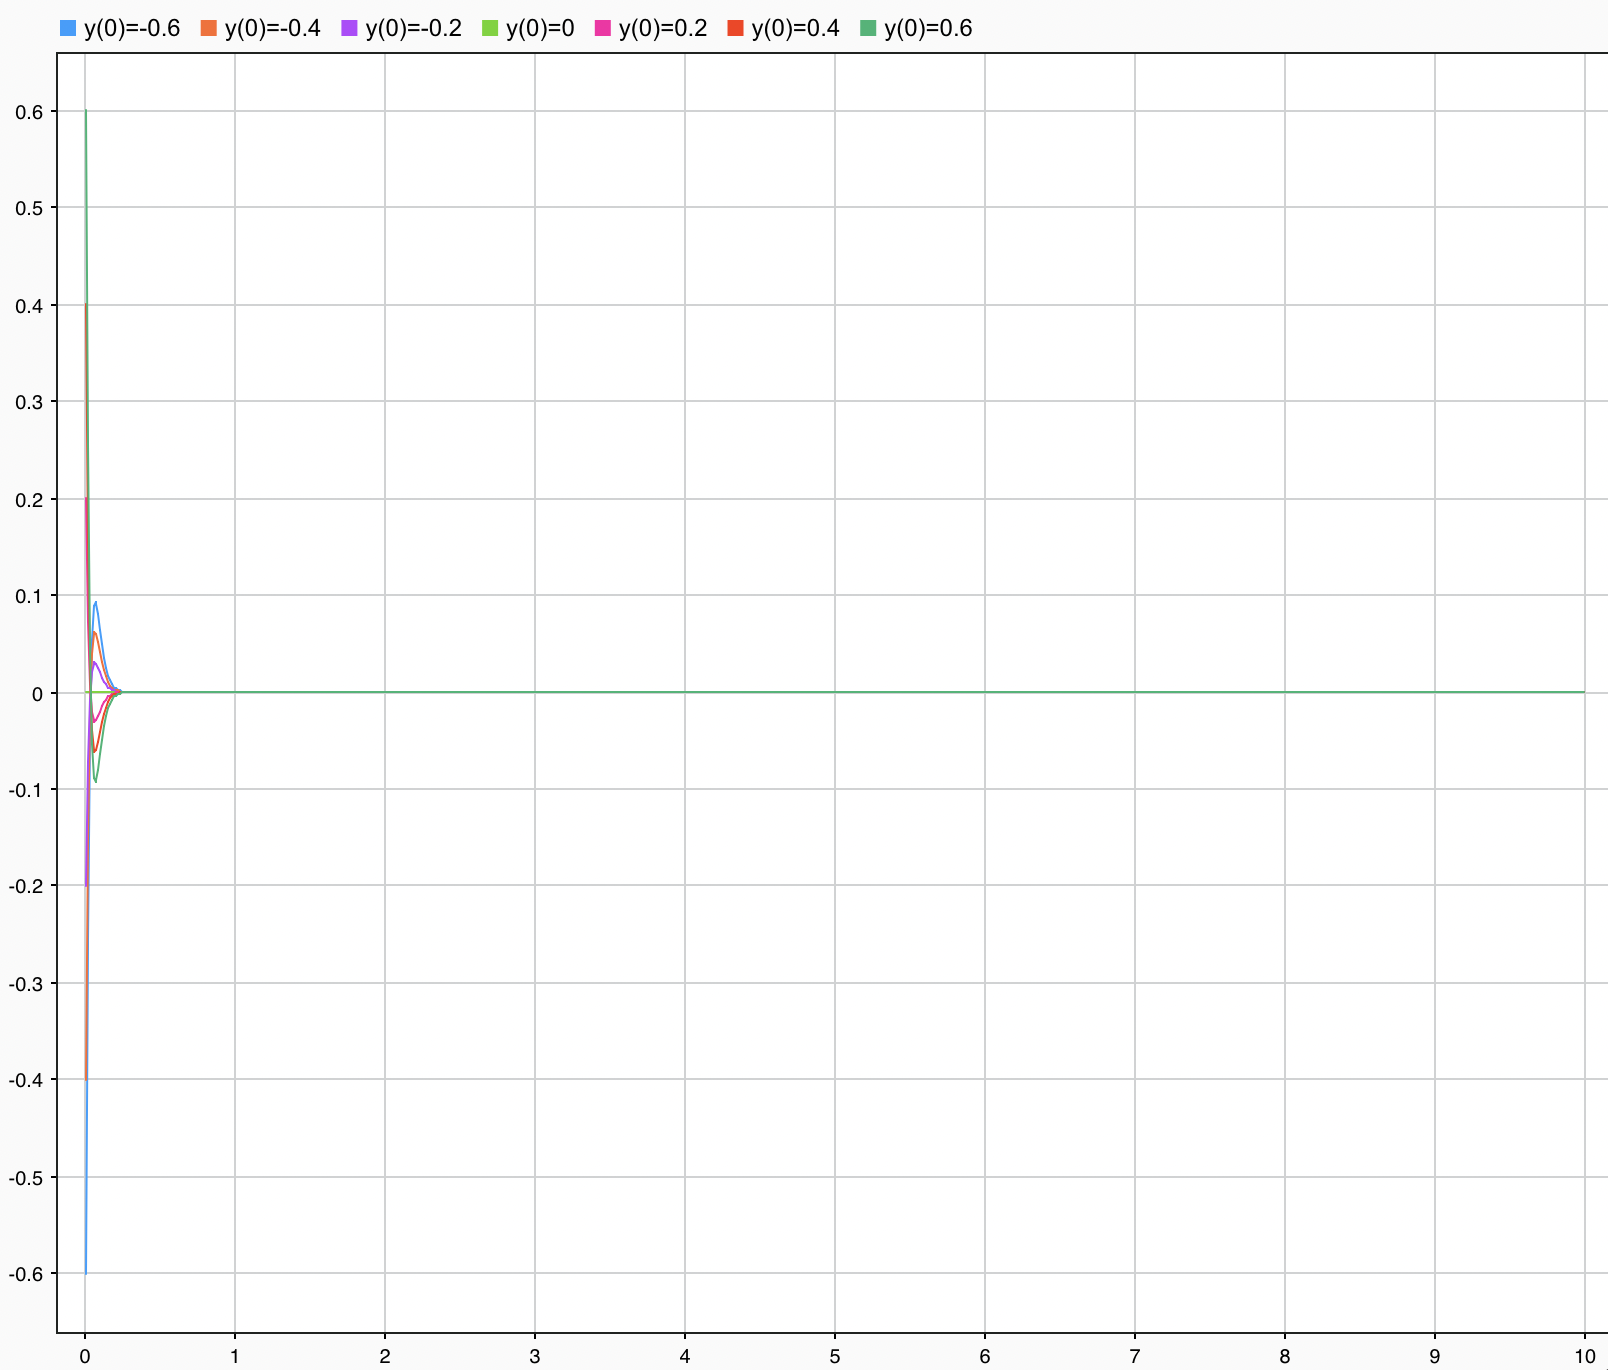
\includegraphics[width=\linewidth]{img22.png}
          \caption{Position}
        \end{subfigure}
        \begin{subfigure}{0.4\linewidth}
          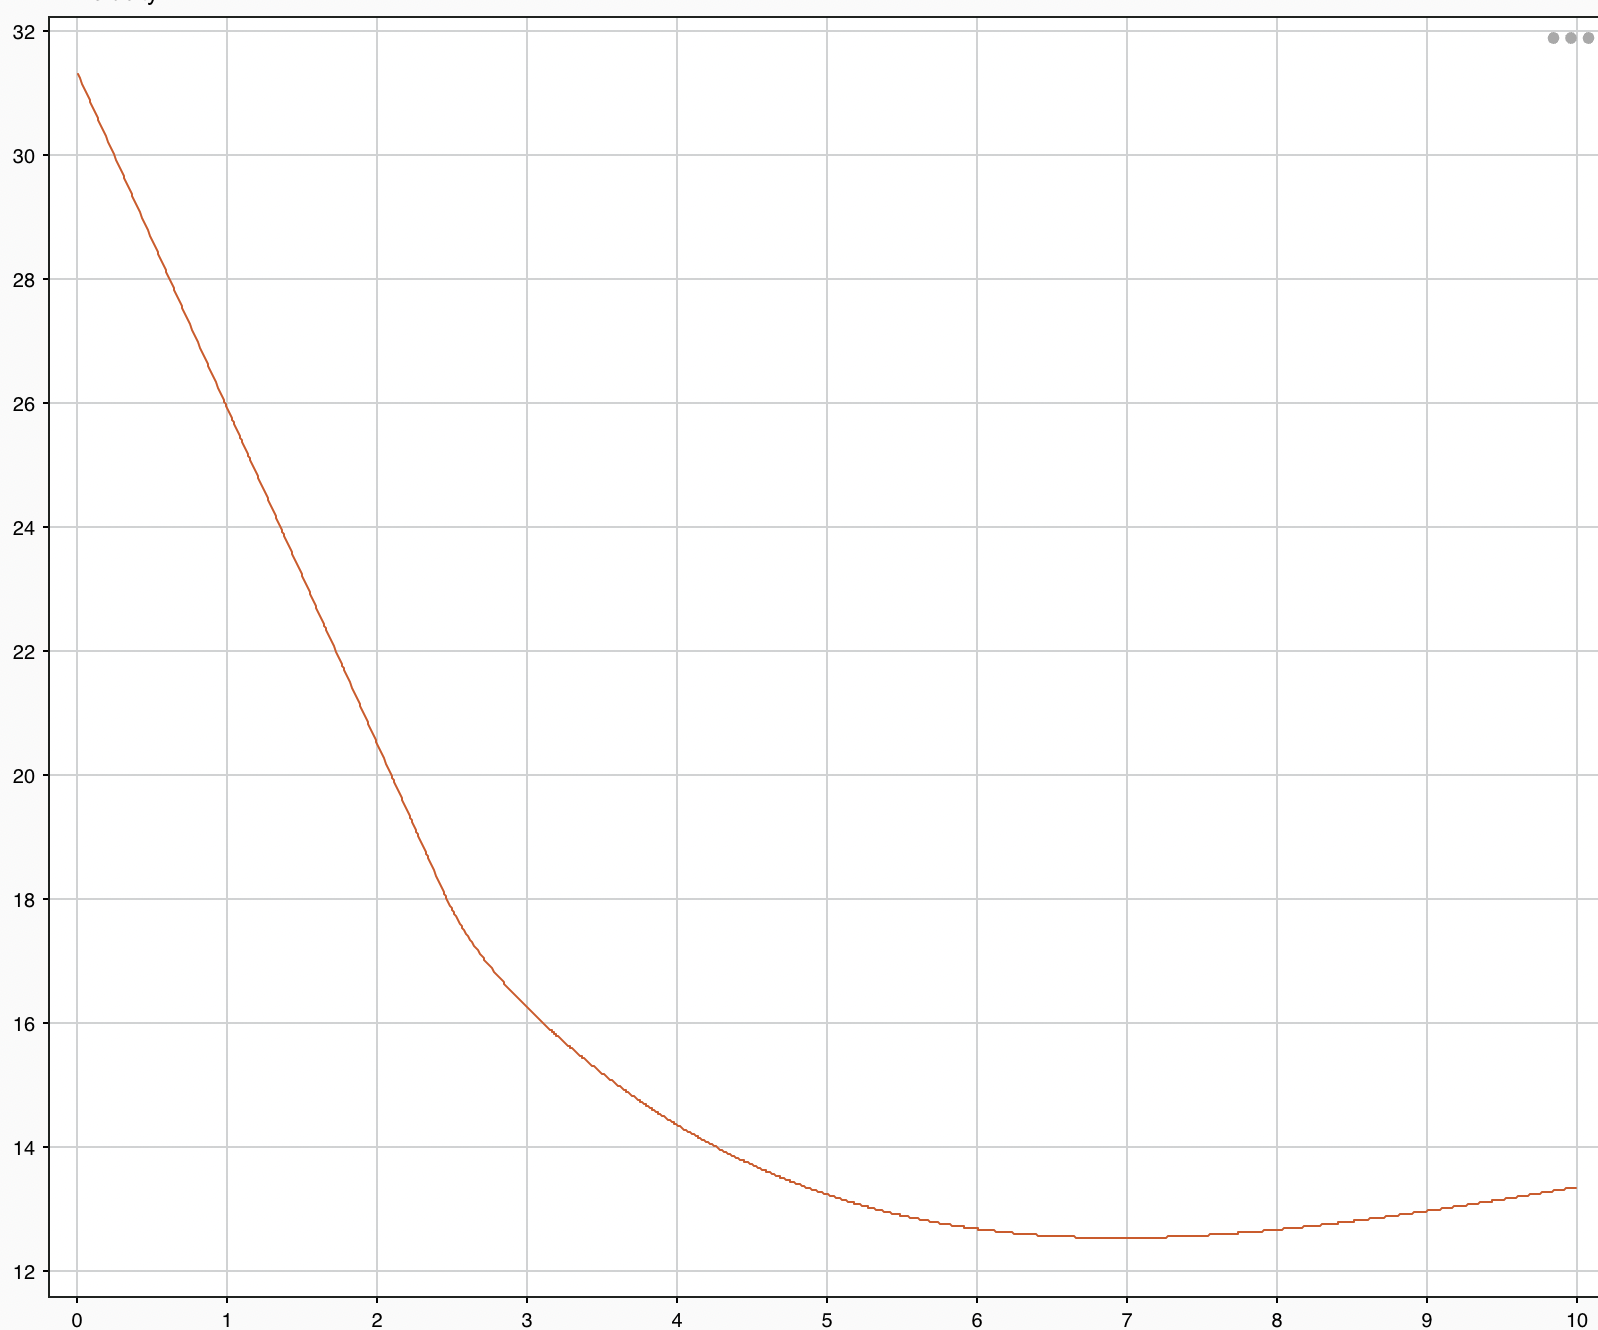
\includegraphics[width=\linewidth]{img23.png}
          \caption{Velocity}
        \end{subfigure}
        \caption{Plots for v(0)=70 mph}
  \end{figure}

  Next we must observe what happens when we decrease the speed of the velocity controller. I will not do this by decreasing the  
  maximum acceleration created by the saturation block, as that does not realistically model the behavior of a car
  Rather, I will increasing the $k_D$ constant in the PID controller .
  Seeing as within the acceptable range, all starting conditions have similar behaviors, let us obsere what happens when we reduce the speed of the velocity controller For
  $y(0)=0.6$ and $v(0)=17.5mph$. \newline

  We see in the figure below that changing the speed of the veloicty controller does not change the output y in any significant way.
  It is almost impossible to distinguish between the different lines for different speeds of the controller. Meanwhile, we can confirm that the controllers with higher $k_D$
  are indeed working slower with the subplots.

  \begin{figure}[h!]
    \centering
    \begin{subfigure}{0.4\linewidth}
      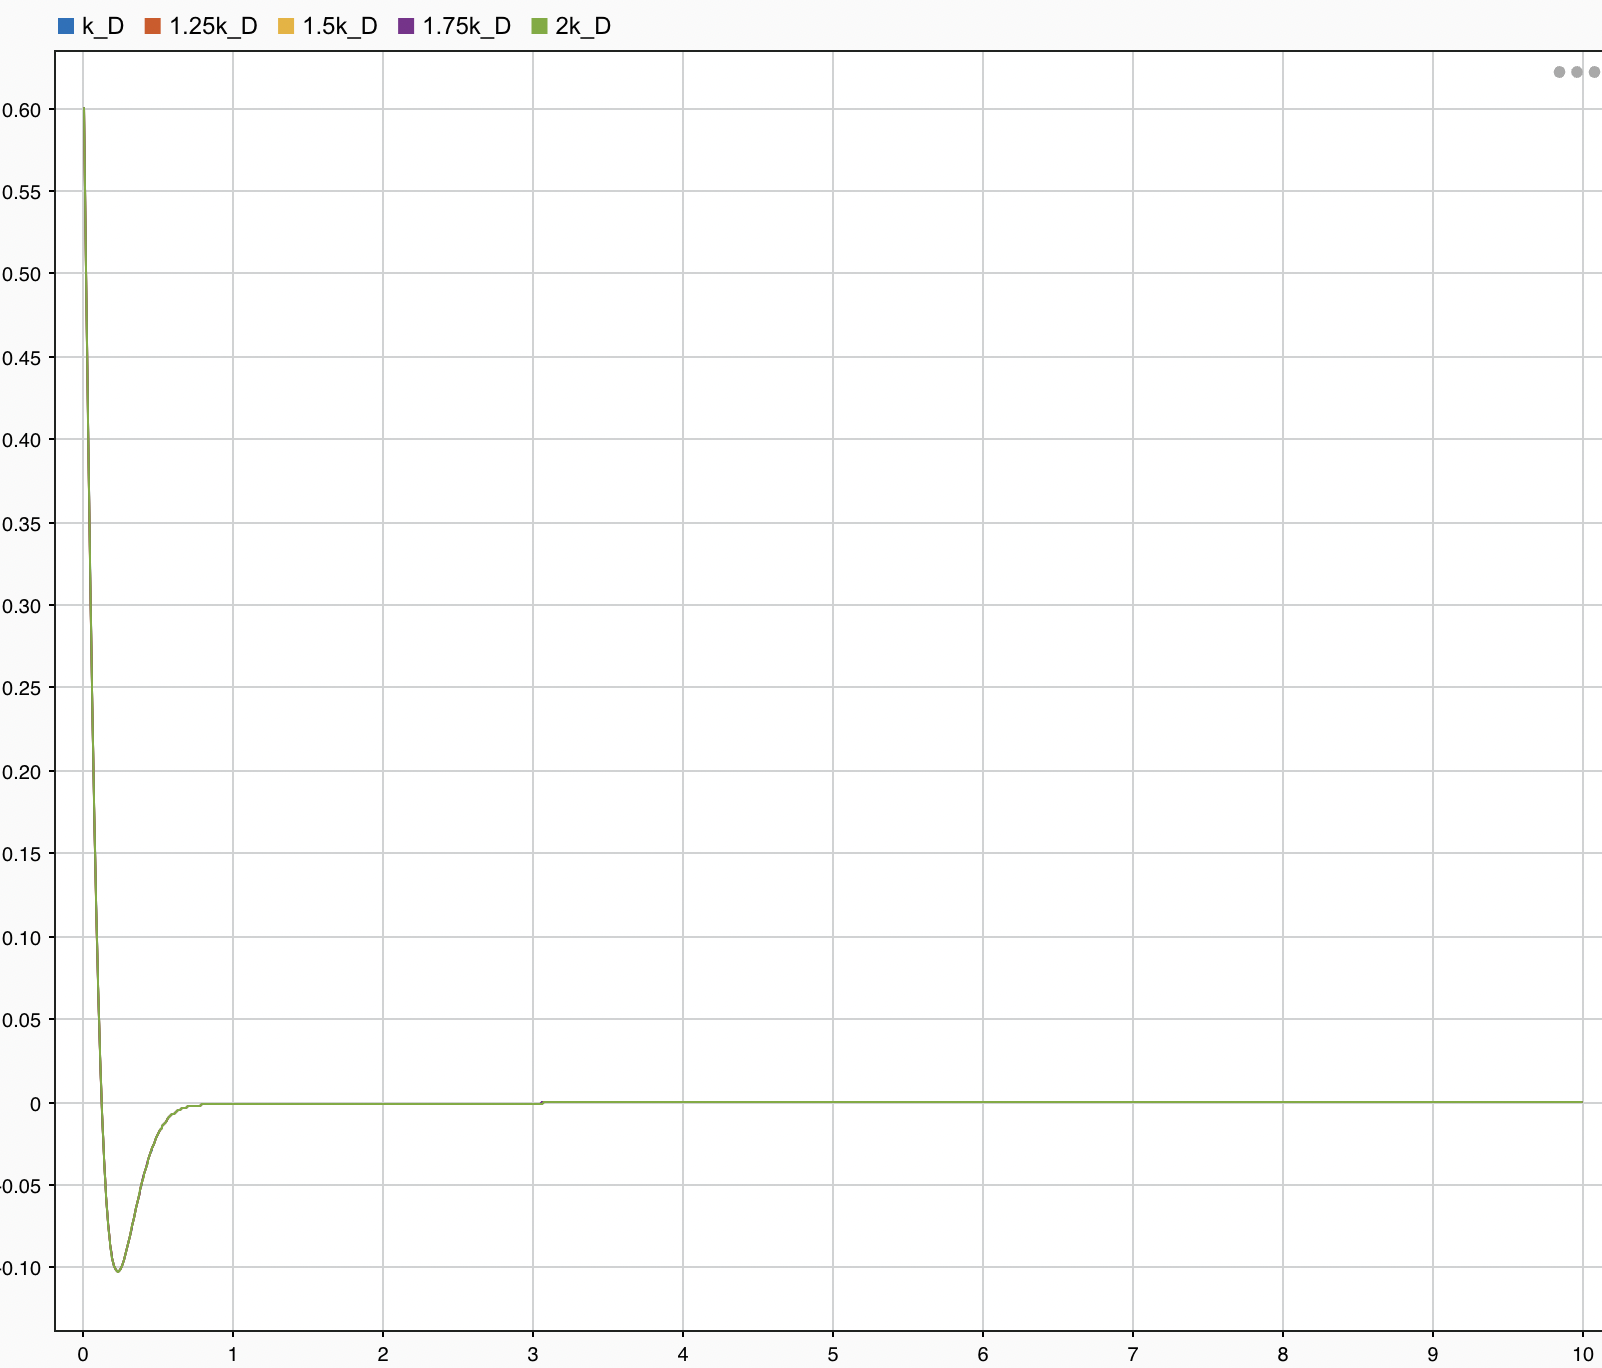
\includegraphics[width=\linewidth]{img24.png}
      \caption{Position}
    \end{subfigure}
    \begin{subfigure}{0.4\linewidth}
      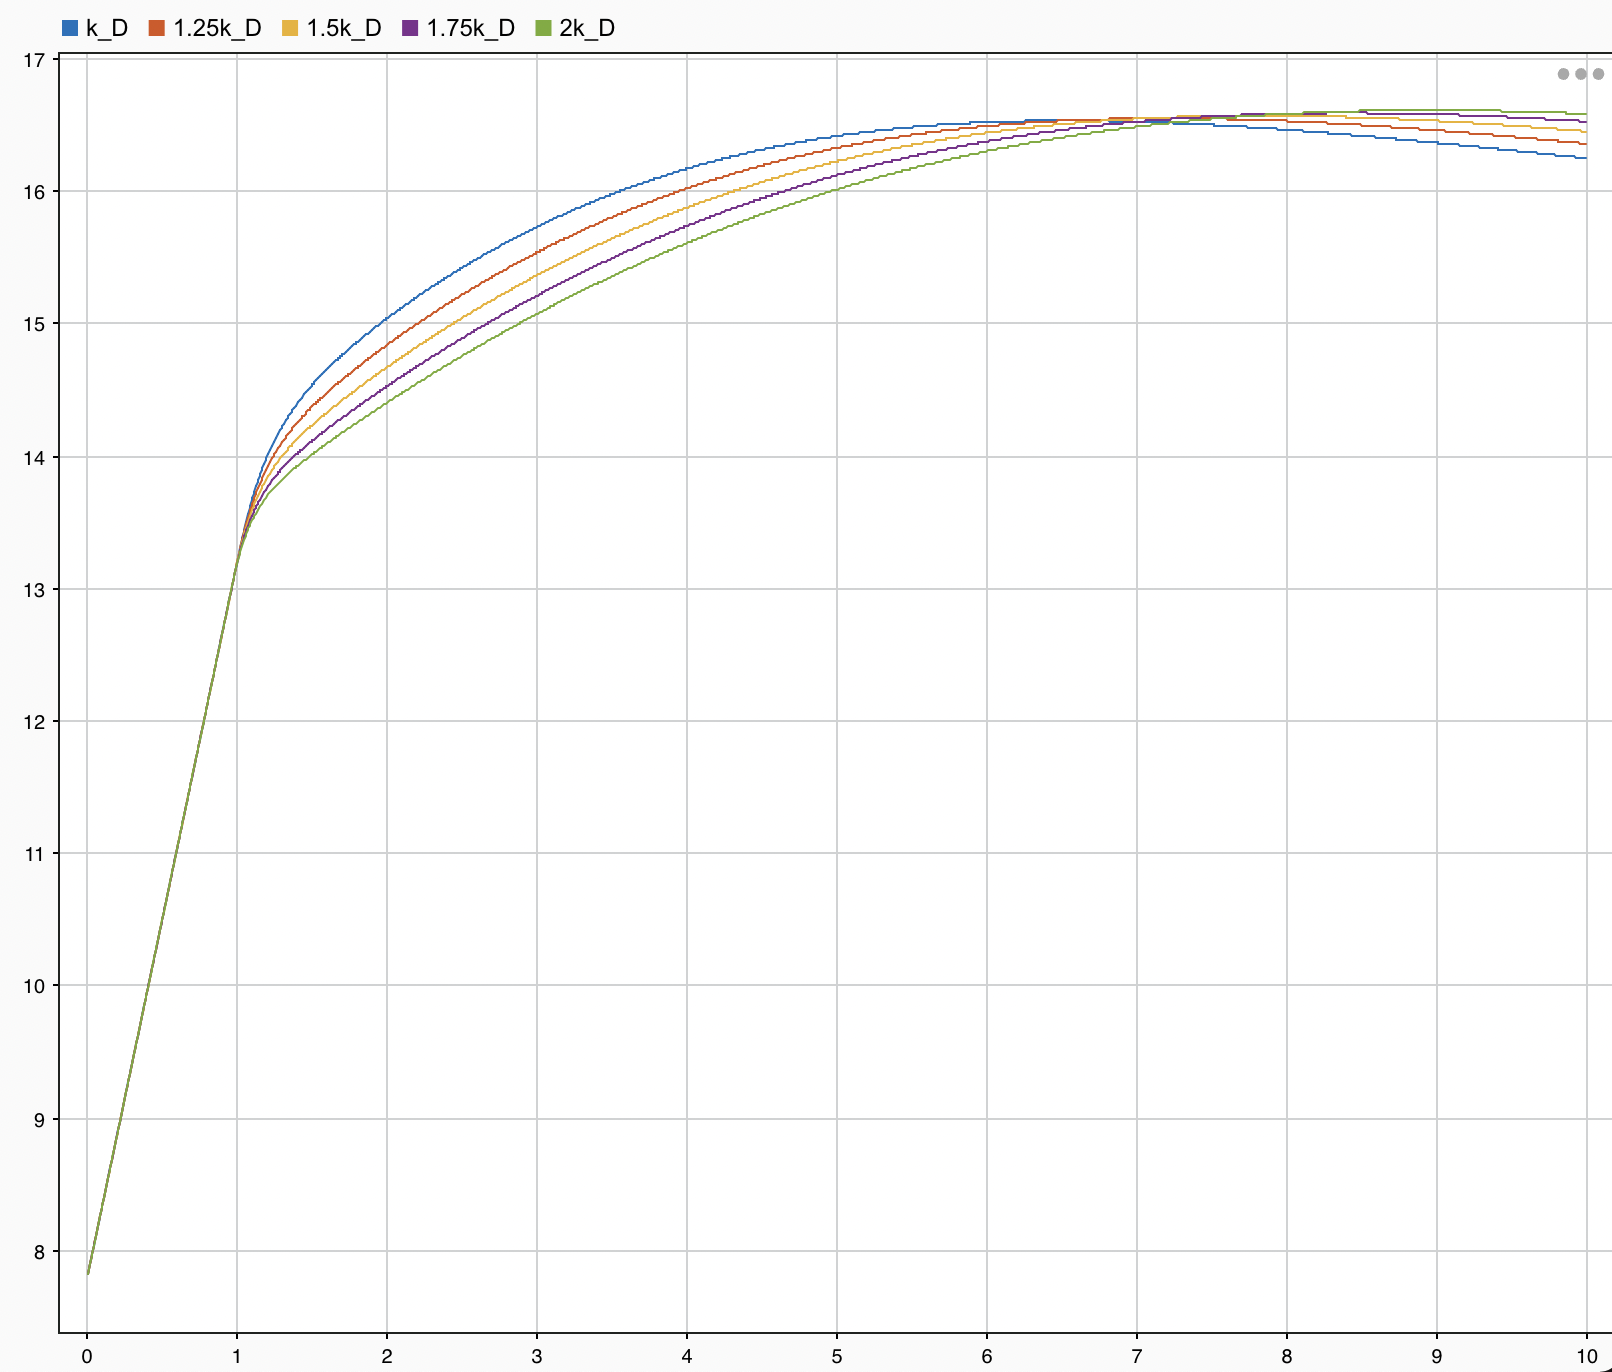
\includegraphics[width=\linewidth]{img25.png}
      \caption{Velocity}
    \end{subfigure}
    \caption{Plots with varying speeds of veloicty controller}
\end{figure}

\end{proof}

\subsection*{Problem 6}
How does the answer to the previous question changes as the commanded velocity in-
creases? Provide some plots to justify your answer.

\begin{proof}[Solution]

Let us assume the inital velocity is 0 and inital $y$ is 0.6 as we know our controller has relatively the same behavior in its acceptable range.
Now, let us plot the effect of decreasing the speed of the controller as the commanded velocity increases.

\begin{figure}[h!]
    \centering
    \begin{subfigure}{0.4\linewidth}
      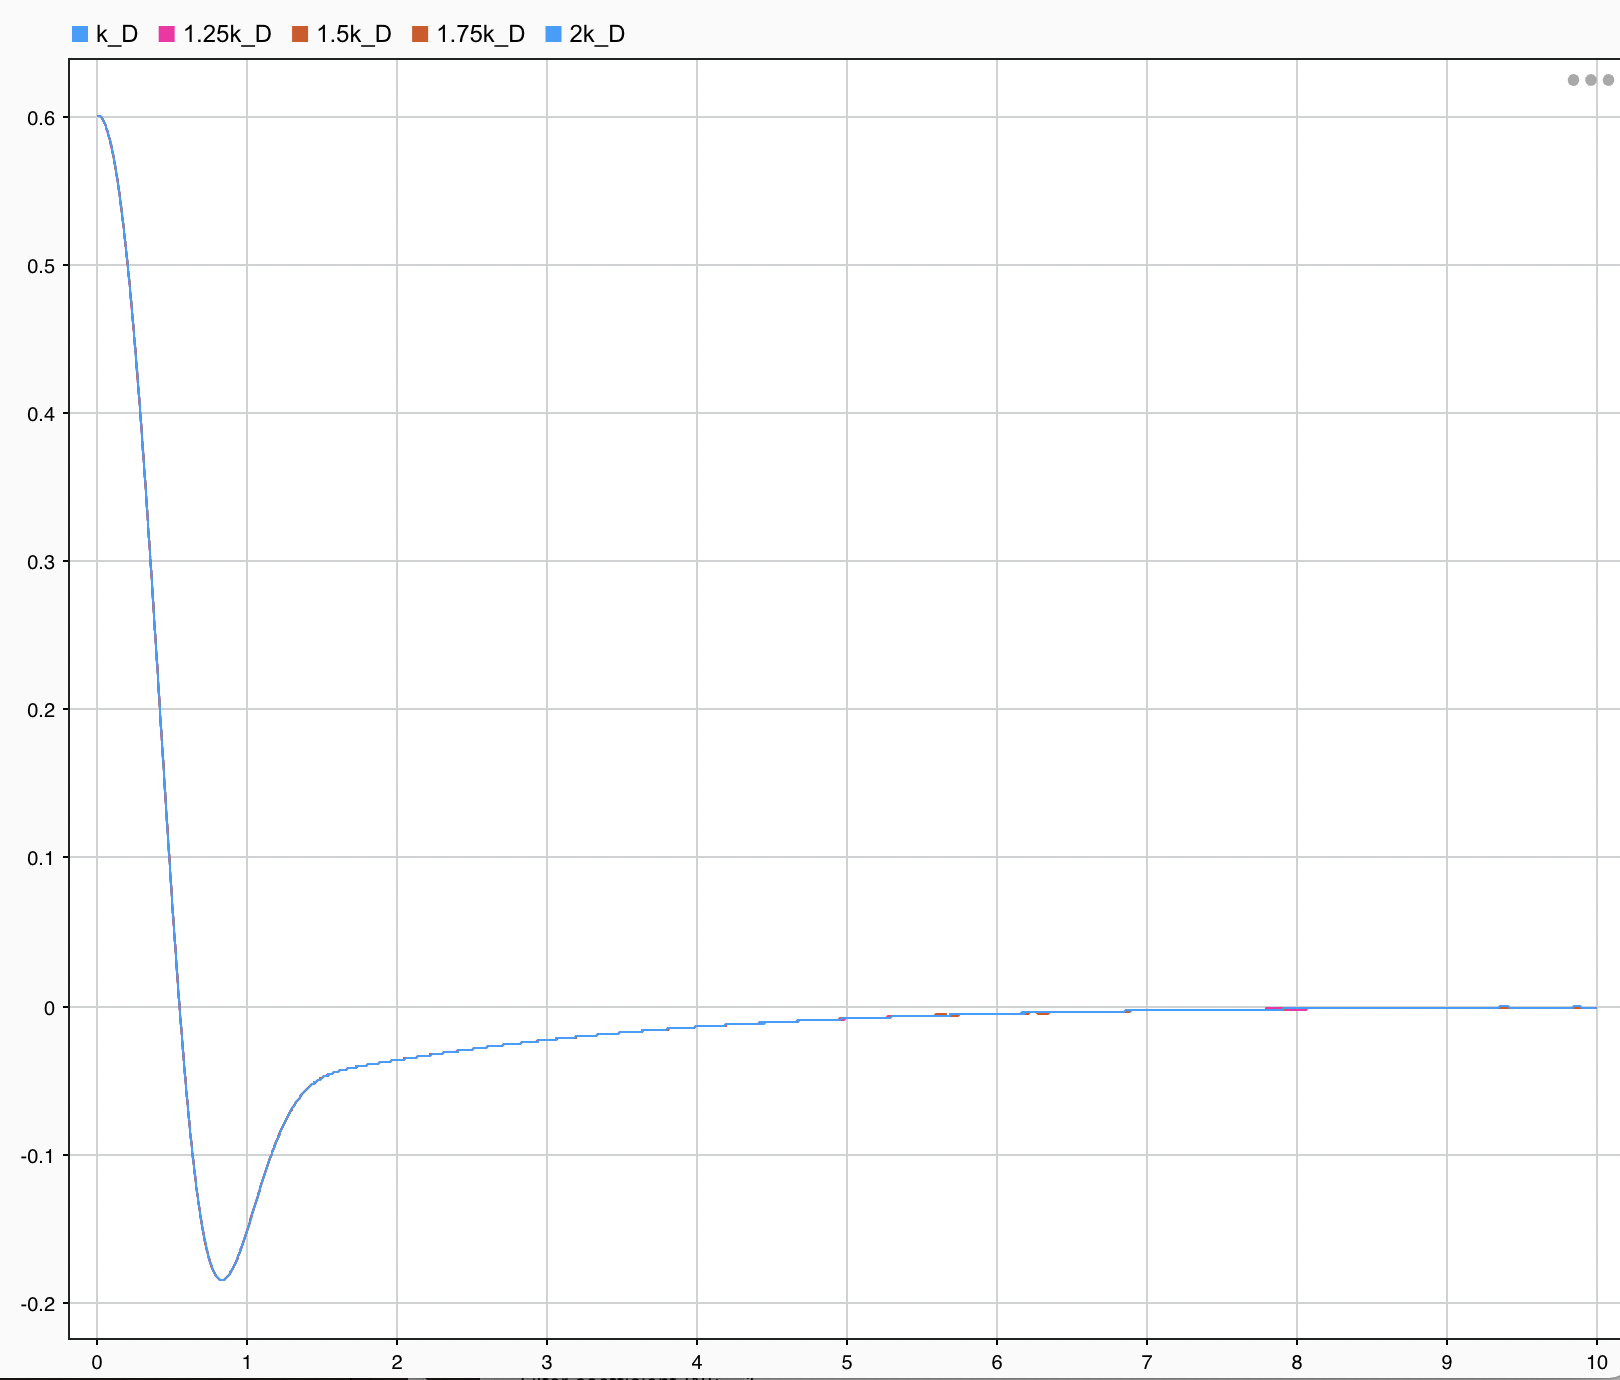
\includegraphics[width=\linewidth]{img26.png}
      \caption{Position}
    \end{subfigure}
    \begin{subfigure}{0.4\linewidth}
      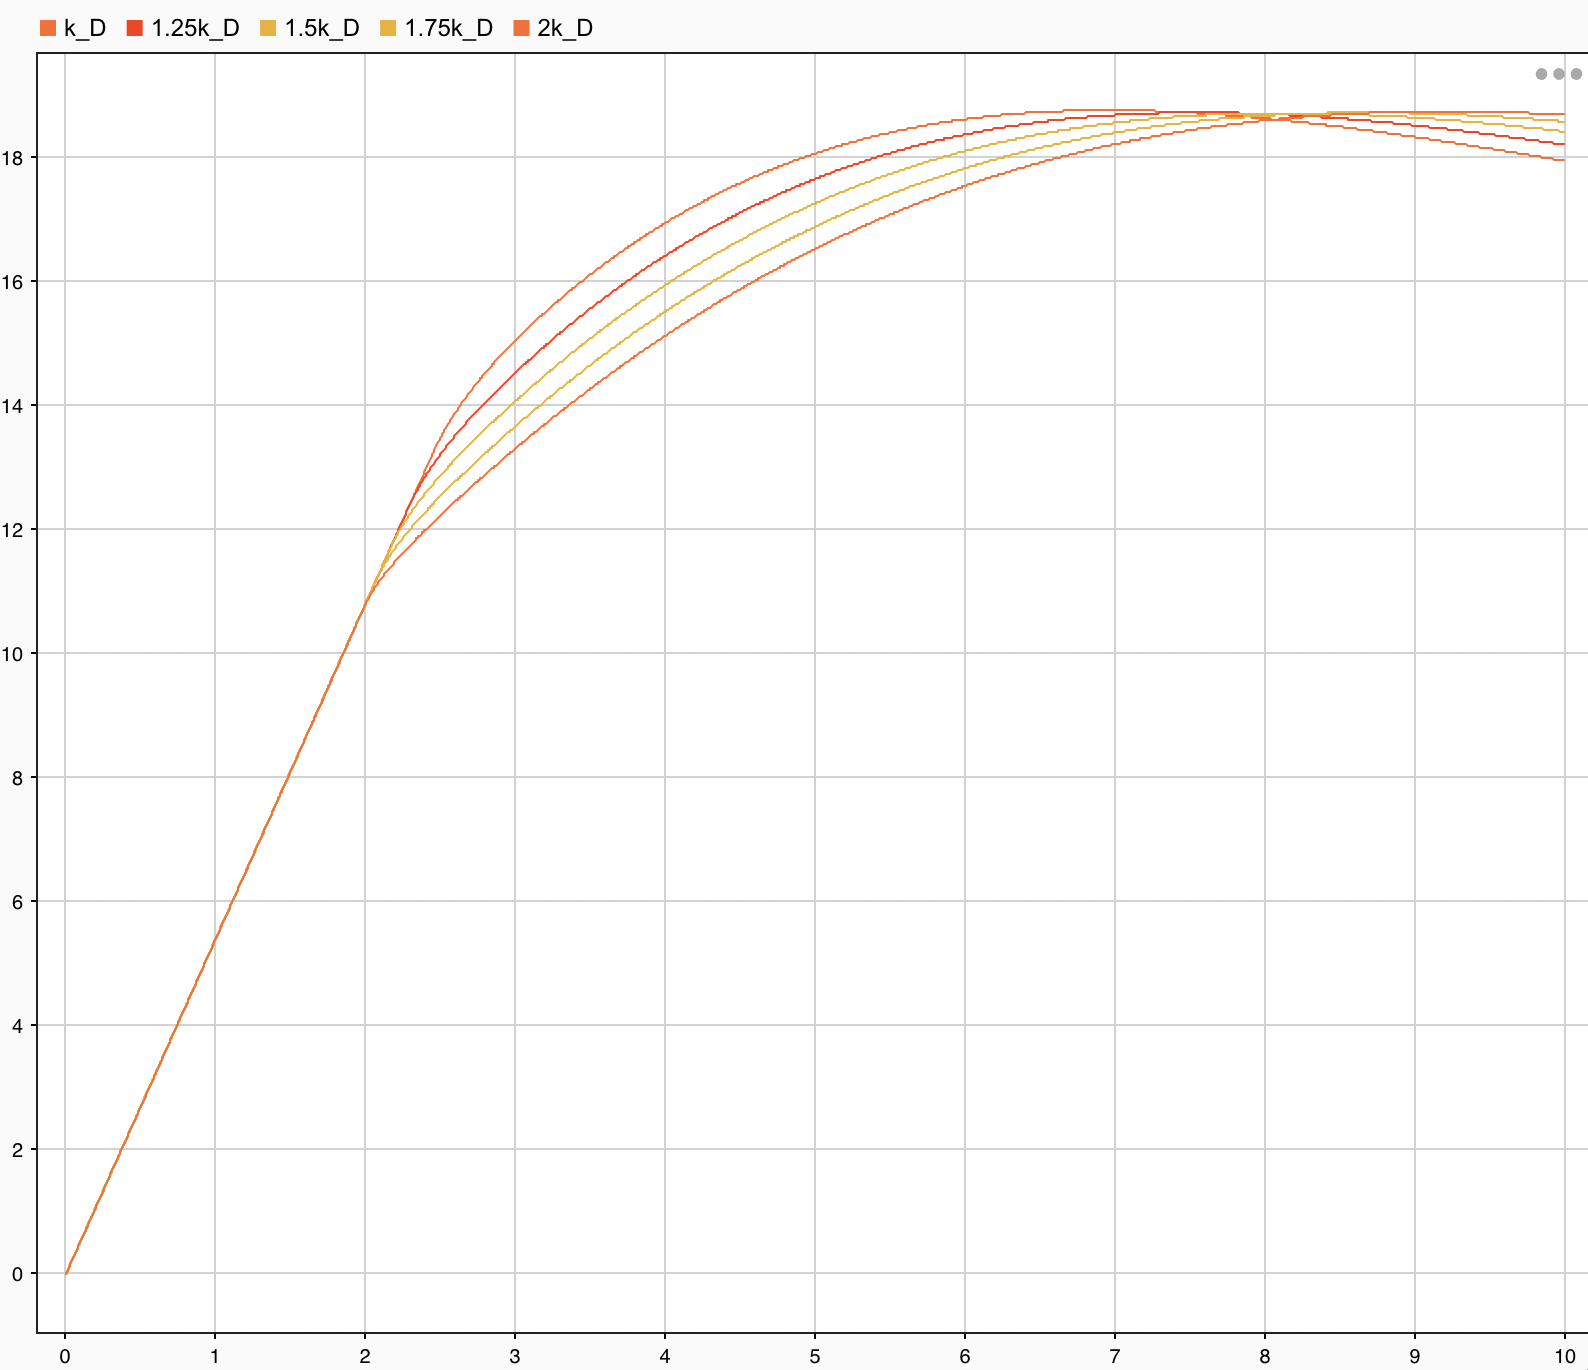
\includegraphics[width=\linewidth]{img27.png}
      \caption{Velocity}
    \end{subfigure}
    \caption{Command Velocity of 35mph}
\end{figure}

\begin{figure}[h!]
    \centering
    \begin{subfigure}{0.4\linewidth}
      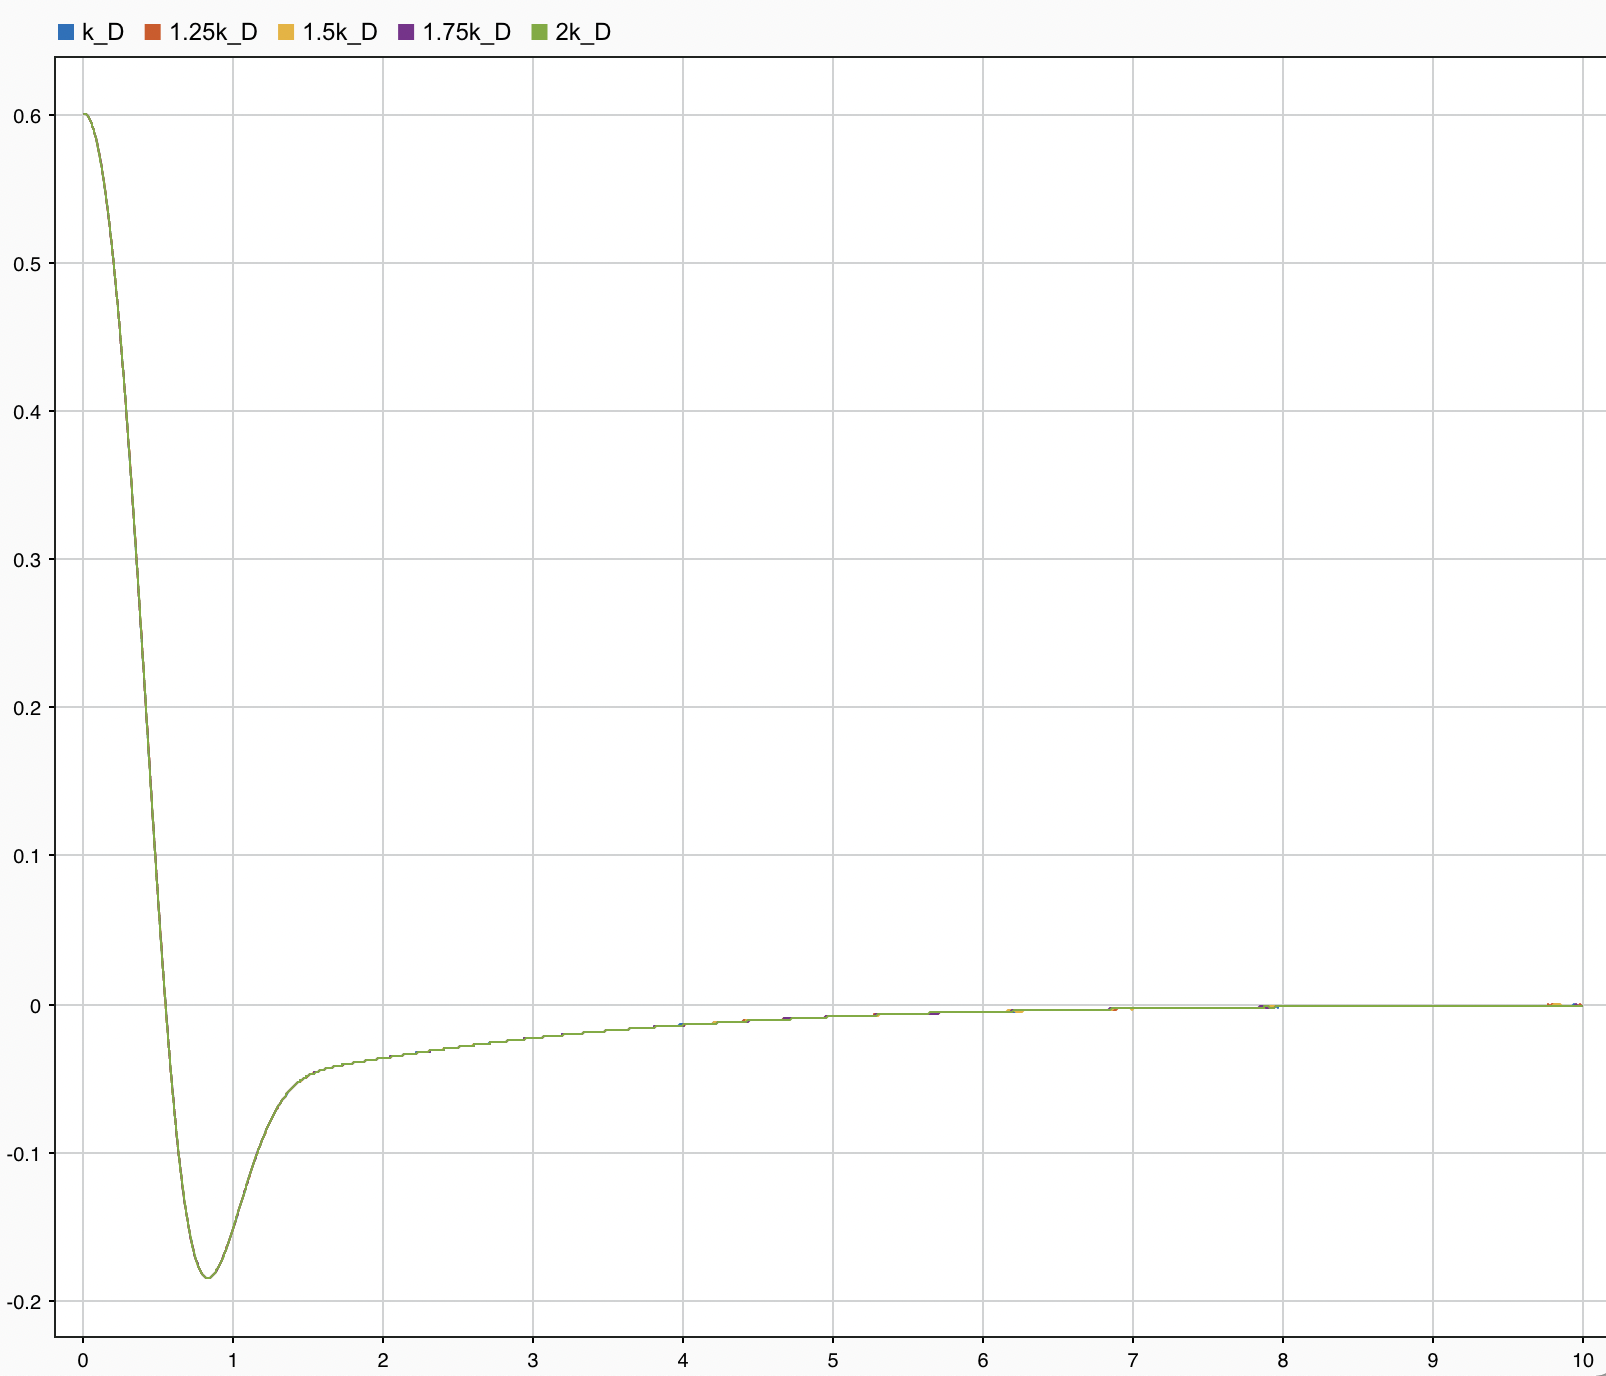
\includegraphics[width=\linewidth]{img28.png}
      \caption{Position}
    \end{subfigure}
    \begin{subfigure}{0.4\linewidth}
      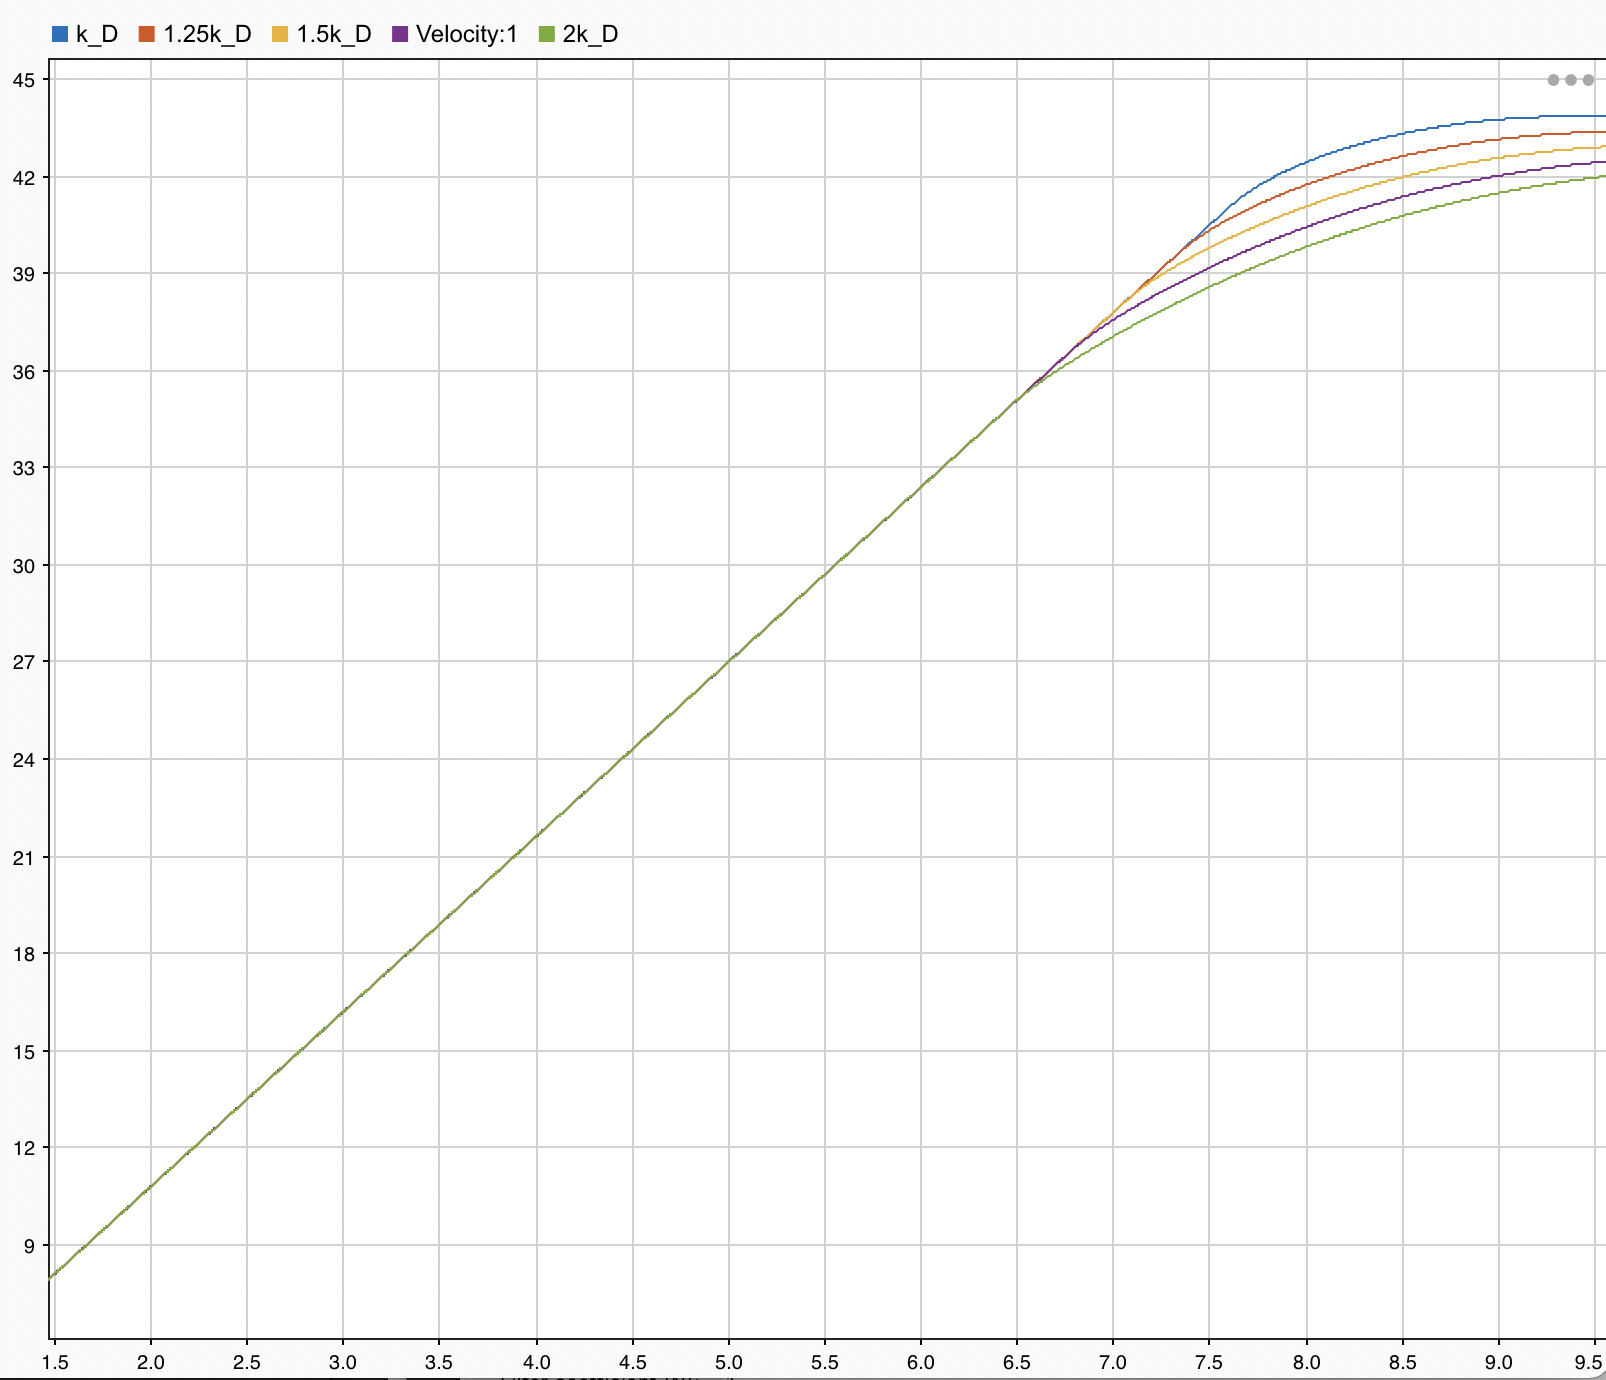
\includegraphics[width=\linewidth]{img29.png}
      \caption{Velocity}
    \end{subfigure}
    \caption{Command Velocity of 70mph}
\end{figure}

\begin{figure}[h!]
    \centering
    \begin{subfigure}{0.4\linewidth}
      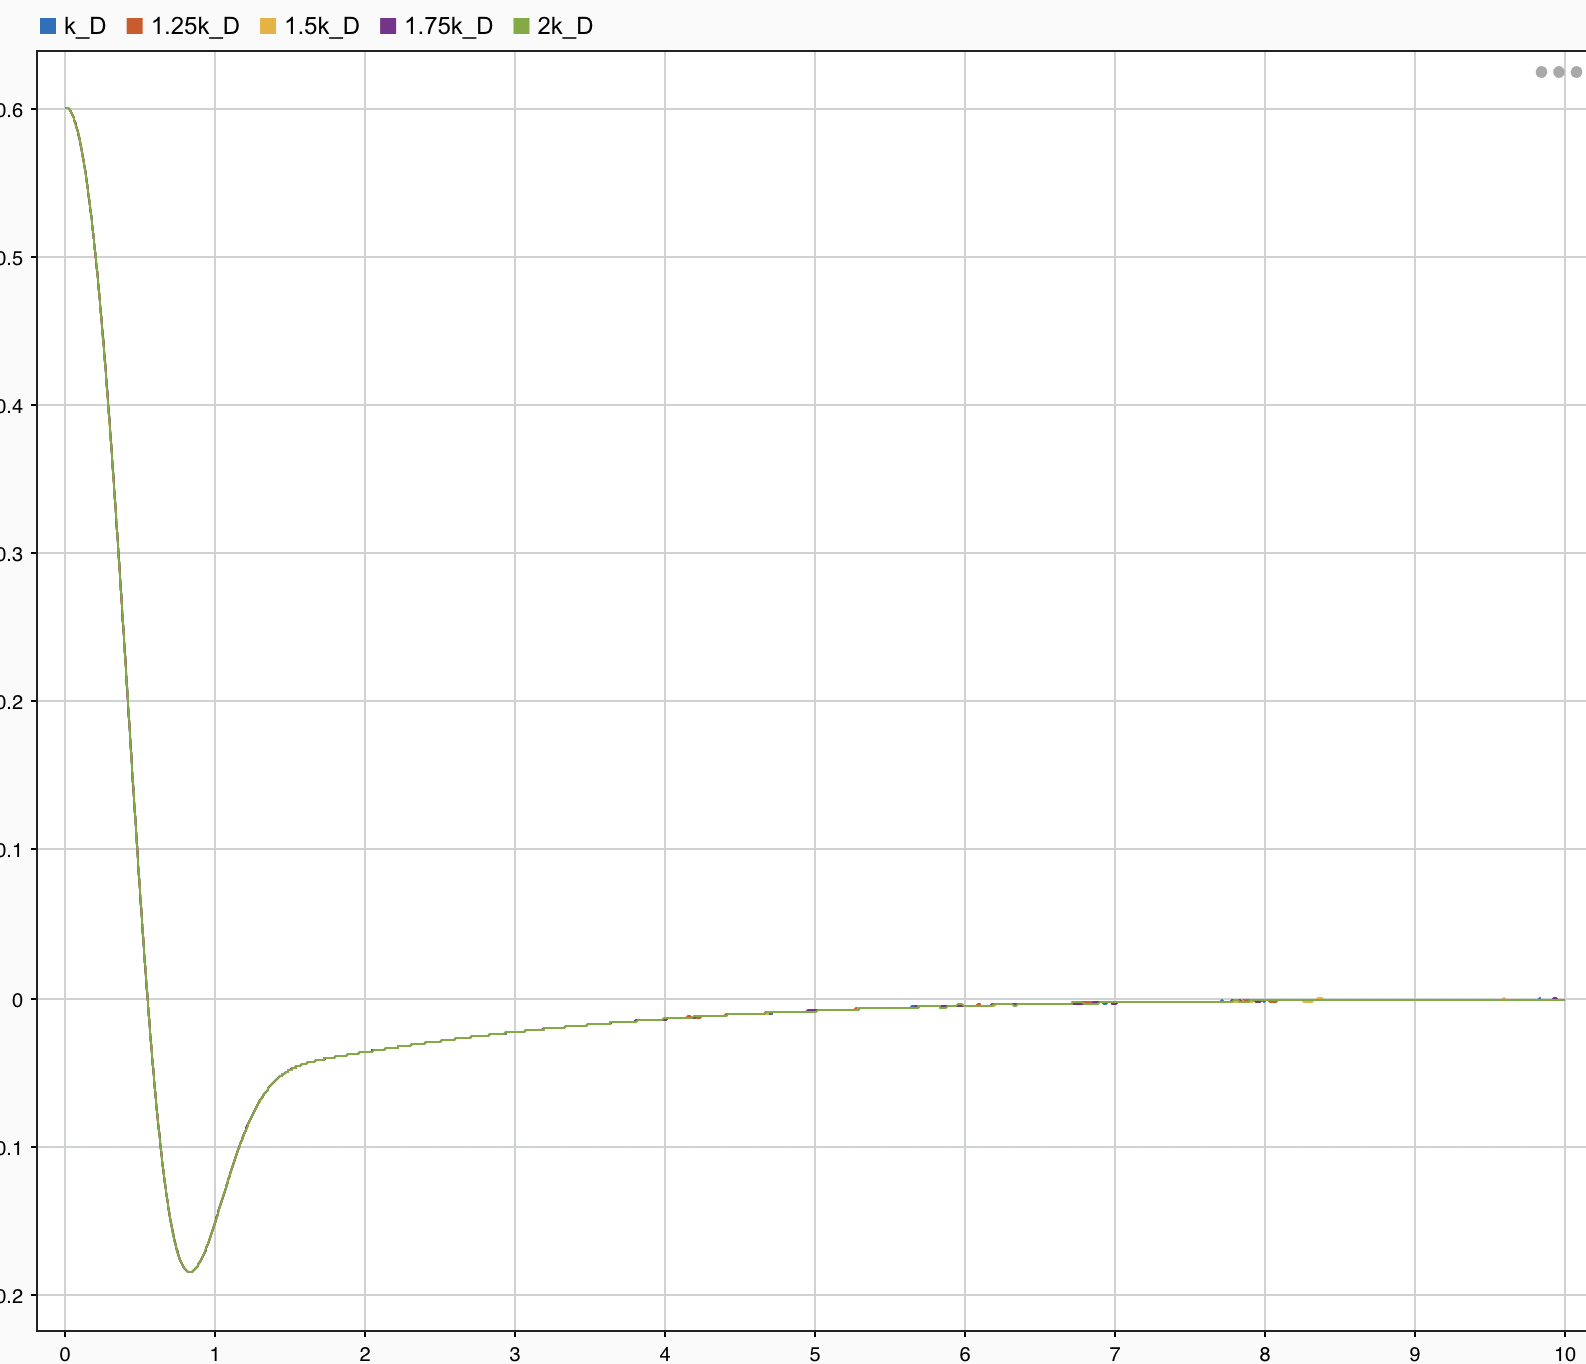
\includegraphics[width=\linewidth]{img30.png}
      \caption{Position}
    \end{subfigure}
    \begin{subfigure}{0.4\linewidth}
      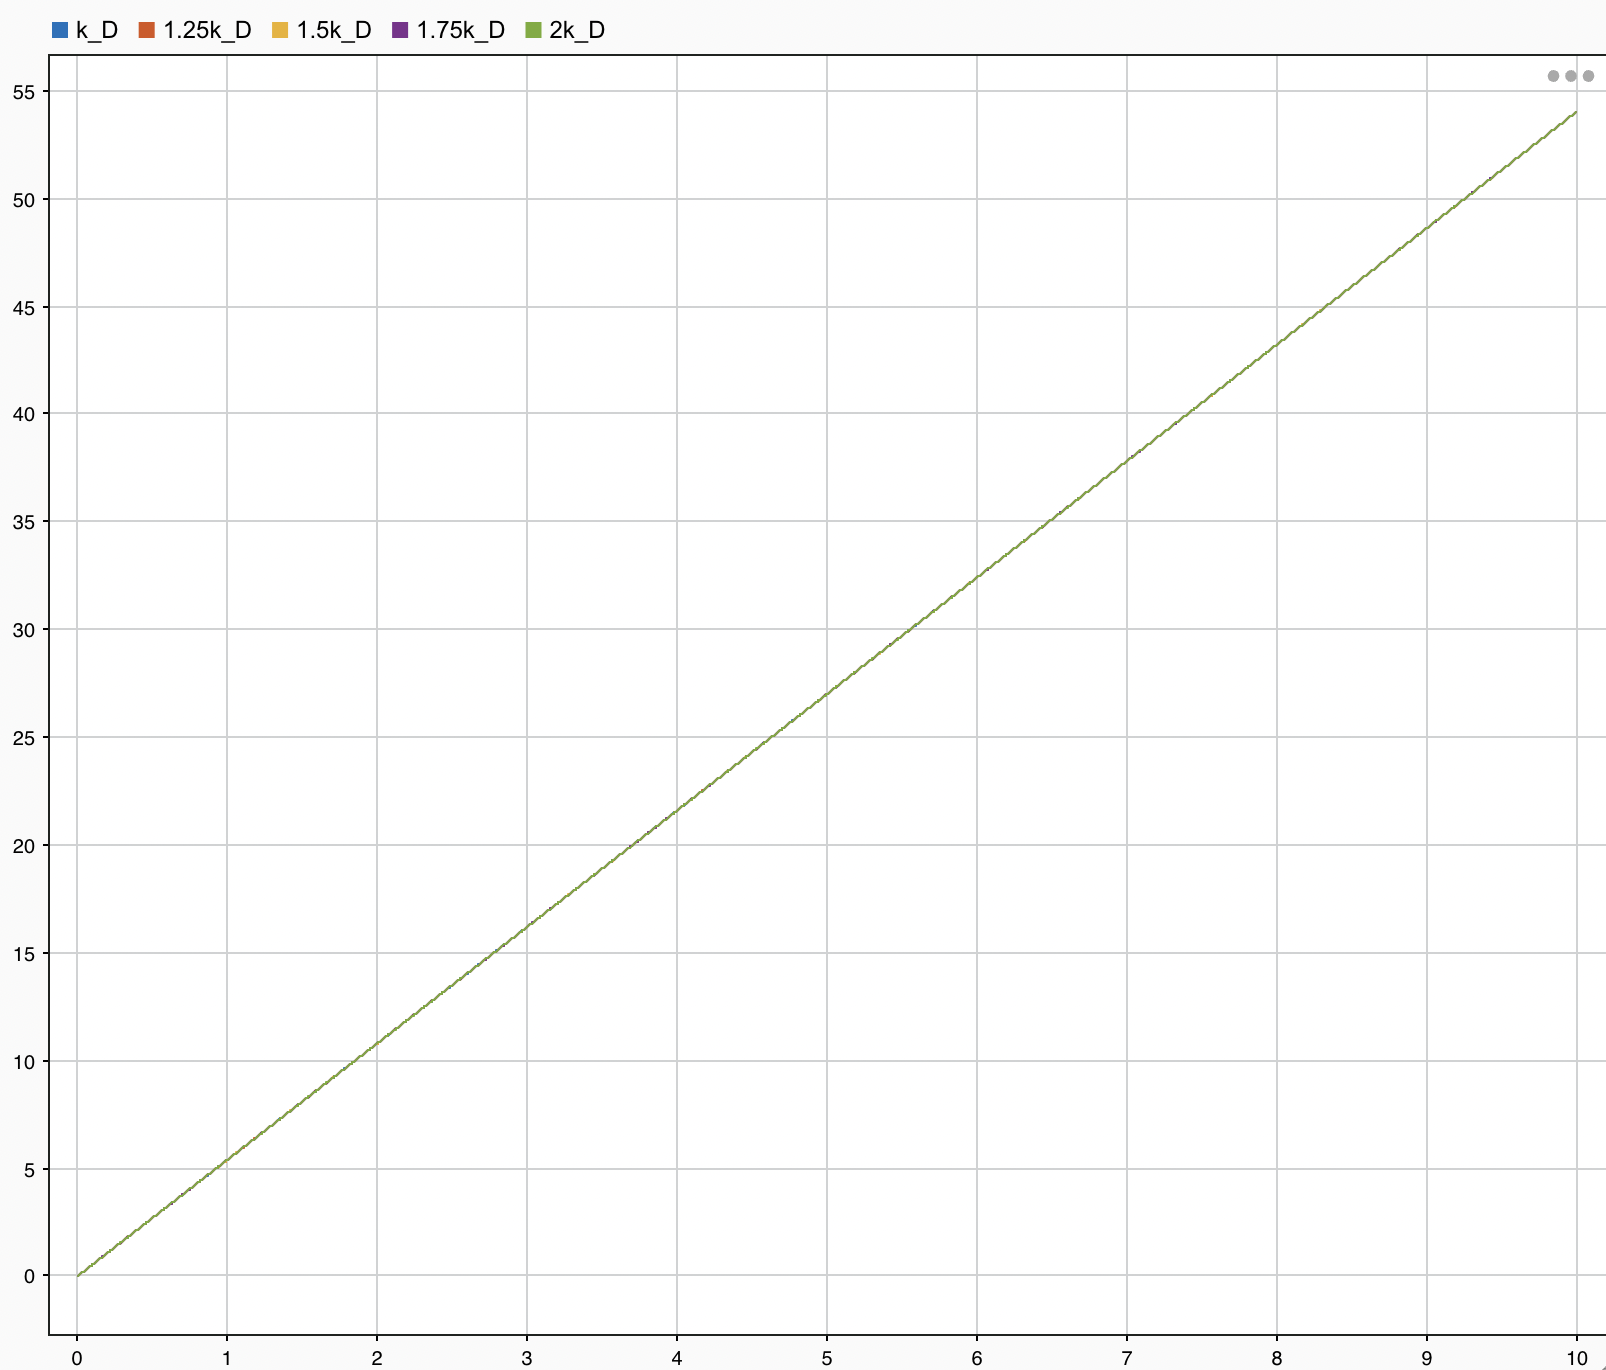
\includegraphics[width=\linewidth]{img31.png}
      \caption{Velocity}
    \end{subfigure}
    \caption{Command Velocity of 140mph}
\end{figure}


We see in the figures above that increasing command velocity does not change the answer to number 5 for values that are 
within the acceptable range of the controller, and even out of the range of the controller, as even with a velocity of 140mph, different lines for position across different $k_D$ are essentially negligible. However, this is simply due to the fact that acceleration is capped in the controller for velocity, so we have a linear increase in velocity, or constant acceleration across all plots at such high command velocity.
Thus, the answer to the previous problem does not change.
\end{proof}

\end{document}